%------------------------------------------------Main.tex % the one that you should compile ;)

\documentclass[a4paper,12pt,oneside]{report}

% Packages
\usepackage[T1]{fontenc}
\usepackage[utf8]{inputenc}
\usepackage[english]{babel}
\usepackage{graphicx}
\usepackage[top=3cm,bottom=4cm,left=3cm,right=3cm]{geometry}
\usepackage{fancyhdr}
\usepackage{enumitem}
\usepackage{soul}
\usepackage{xcolor}
\usepackage{titlesec}
\usepackage{titling}
\usepackage{tcolorbox}
\usepackage{url}
\usepackage{multirow}
\usepackage{array}
\usepackage{tabularx}
\usepackage{longtable}
\usepackage{makecell}
\usepackage{amssymb}
\usepackage{amsfonts}
\usepackage{amsmath}
\usepackage{listings}
\usepackage{caption}
\usepackage{acro}
\usepackage[section]{placeins}
\usepackage{float}
\usepackage{pifont}
\usepackage{version}
\usepackage{lettrine}
\usepackage{arabtex}
\usepackage{bibtopic}
\usepackage{ulem}
\usepackage{newfloat}
\usepackage{hyperref}
\usepackage{indentfirst}
\usepackage{changepage}
\usepackage{acro}


% Custom Commands
\newcommand{\HRule}{\textcolor{lightgray}{\rule{15.5 cm}{0.12 cm}}}
\newcommand{\Hrule}{\textcolor{lightgray}{\rule{13.5 cm}{0.15 cm}}}
\newcommand{\customizeNumber}{\fontsize{40}{40}\usefont{U}{eur}{b}{n}}
\newcommand{\chapterNumber}{\fontsize{12}{12}\usefont{U}{b}{n}}

% Package Configurations
% packages-config.tex

% Define a style for CPP
\lstdefinestyle{cppStyle}{
  language=C++,
  basicstyle=\ttfamily\small,
  keywordstyle=\color{blue},
  commentstyle=\color{green!50!black},
  stringstyle=\color{red},
  showstringspaces=false,
  breaklines=true,
  frame=single,
  numbers=left,
  numberstyle=\tiny\color{gray}
}

% Define a style for JSON
\lstdefinelanguage{json}{
    keywords={true,false,null},
    keywordstyle=\color{blue}\bfseries,
    sensitive=false,
    comment=[l]{//},
    morecomment=[s]{/*}{*/},
    string=[b]",
    stringstyle=\color{purple},
    literate=
      *{0}{{{\color{blue}0}}}{1}
       {1}{{{\color{blue}1}}}{1}
       {2}{{{\color{blue}2}}}{1}
       {3}{{{\color{blue}3}}}{1}
       {4}{{{\color{blue}4}}}{1}
       {5}{{{\color{blue}5}}}{1}
       {6}{{{\color{blue}6}}}{1}
       {7}{{{\color{blue}7}}}{1}
       {8}{{{\color{blue}8}}}{1}
       {9}{{{\color{blue}9}}}{1}
}

% Define a style for listings using the JSON language
\lstdefinestyle{jsonStyle}{
    language=json,
    basicstyle=\ttfamily\small,
    numbers=left,
    numberstyle=\tiny,
    stepnumber=1,
    numbersep=5pt,
    showstringspaces=false,
    breaklines=true,
    frame=single,
    backgroundcolor=\color{gray!10},
    rulecolor=\color{black},
    stringstyle=\color{purple},
    commentstyle=\color{green},
    keywordstyle=\color{blue}\bfseries,
    morekeywords={true, false, null}
}

% Custom title format for sections
\titleformat{\section}[block]
  {\huge\bfseries}
  {\color{gray} \thesection \hspace{10pt}\vline}
  {10pt}
  {}

\newcounter{listingcounter}
\DeclareFloatingEnvironment[fileext=lor]{Rule}


\fancypagestyle{acronyms}{
    \fancyhf{} % Clear header and footer
    \fancyhead[R]{\textit{GLOSSARY OF ACRONYMS}} % Header content
    \renewcommand{\headrulewidth}{2pt} % Header rule
    \fancyfoot[C]{\thepage} % Footer content (page number)
}

\fancypagestyle{intro}{
    \fancyhf{} % Clear header and footer
    \fancyhead[R]{\textit{GENERAL INTRODUCTION}} % Header content
    \renewcommand{\headrulewidth}{2pt} % Header rule
    \fancyfoot[C]{\thepage} % Footer content (page number)
}

%Subsubsection creation BEGIN
\titleclass{\subsubsubsection}{straight}[\subsection]

\newcounter{subsubsubsection}[subsubsection]
\renewcommand\thesubsubsubsection{\thesubsubsection.\arabic{subsubsubsection}}
\renewcommand\theparagraph{\thesubsubsubsection.\arabic{paragraph}} % optional; useful if paragraphs are to be numbered

\renewcommand\thesection{\arabic{section}}

\titleformat{\subsubsubsection}
  {\normalfont\normalsize\bfseries}{\thesubsubsubsection}{1em}{}
\titlespacing*{\subsubsubsection}
{0pt}{3.25ex plus 1ex minus .2ex}{1.5ex plus .2ex}

\makeatletter
\renewcommand\paragraph{\@startsection{paragraph}{5}{\z@}%
  {3.25ex \@plus1ex \@minus.2ex}%
  {-1em}%
  {\normalfont\normalsize\bfseries}}
\renewcommand\subparagraph{\@startsection{subparagraph}{6}{\parindent}%
  {3.25ex \@plus1ex \@minus .2ex}%
  {-1em}%
  {\normalfont\normalsize\bfseries}}
\def\toclevel@subsubsubsection{4}
\def\toclevel@paragraph{5}
\def\toclevel@paragraph{6}
\def\l@subsubsubsection{\@dottedtocline{4}{7em}{4em}}
\def\l@paragraph{\@dottedtocline{5}{10em}{5em}}
\def\l@subparagraph{\@dottedtocline{6}{14em}{6em}}
\makeatother

\setcounter{secnumdepth}{4}
\setcounter{tocdepth}{4}
%Subsubsection creation END
% Additional package configurations, if needed

\definecolor{mygray}{rgb}{0.9,0.9,0.9}

% Page Style
\pagestyle{fancy}
\fancyhead[L]{}
\renewcommand{\headrulewidth}{2pt}
\setlength{\headheight}{15pt}
\setlength{\parskip}{0.7em} 

\hypersetup{
  hidelinks=true % This removes frames around hyperlinks
}

% Document
\begin{document}

% Front Page

% Abstract, Signatures, Acknowledgement


% Table of Contents, List of Figures, List of Tables
\pagenumbering{Roman}

%---------------------------------------environment abstract
\newenvironment*{Abstract}{
\renewcommand*{\abstractname}{\Huge \textbf{Abstract}}
\begin{abstract}
\end{abstract}}


%---------------------------------------environment dedication
\newenvironment*{dedication}{
\renewcommand*{\abstractname}{\begin{flushleft}\Huge \textbf{Dedication}\end{flushleft}}
\begin{abstract}
\end{abstract}}

%---------------------------------------environment acknoledgement
\newenvironment*{acknowledgement}{
  \renewcommand*{\abstractname}{\begin{flushleft}\Huge \textbf{Acknowledgement}\end{flushleft}}
  \begin{abstract}
 {}
  \end{abstract}
}
%==========================================================================


%----------------------------------------- Acknowledgement
\newpage

\begin{dedication}

\end{dedication}

%---------------------------------------------Acknowledgement
\begin{acknowledgement}

\end{acknowledgement}

%---------------------------------------------Abstract
\begin{abstract}

      This thesis proposes a methodology for automated path planning for mobile robots in intralogistics 
      environments, taking into consideration environmental obstacles. The proposed path should optimally 
      connect the robot to a nearby target pose, while adhering to the robot’s kinematic constraints. The 
      path planning process should employ an online pattern-based approach, ensuring that the robot’s 
      behaviour is explainable, and all environmental recognition information is utilized during path planning. 
      The thesis aims to reduce the amount of information required for commissioning mobile robots, allowing for 
      broader use cases. The proposed solution will be implemented in the Robotics Application Construction Kit 
      (RACK) framework and evaluated for performance in real-time processing capabilities. The thesis consists 
      of literature review, design and development of the proposed solution, and validation through testing in 
      a simple test environment. The proposed methodology will enable mobile robots to navigate intralogistics 
      environments more efficiently and safely, contributing to increased productivity and dynamic logistics 
      processes.



    
    \textbf{Keywords: Near-Field Path Planning, Optimization Algorithms, Intralogistics, AMR }

    

    

\end{abstract}








\tableofcontents
\listoffigures
\listoftables

% Acronyms
\chapter*{Glossary of Acronyms}


\begin{itemize}
        \item AMR: Autonomous Mobile Robots
        \item AGV: Automated Guided Vehicles
        \item CC: Curvature Change
        \item DWA: Dynamic Window Approach
        \item FL: Fuzzy Logic
        \item GA: Genetic Algorithm
        \item GPP: Global Path Planning
        \item LPP: Local Path Planning
        \item MP: Motion Planning
        \item NN: Neural Network
        \item NFPP: Near-Field Path Planning
        \item OMPL: Open Motion Planning Library
        \item PSO: Particle Swarm Optimization
        \item RACK: Robotics Application Construction Kit
        \item RL: Reinforcement Learning
        \item RNN: Recurrent Neural Network
        \item RRT: Rapidly-exploring Random Tree
        \item SA: Simulated Annealing
\end{itemize}

\newpage







 % TODO: Alphabetical order



\pagestyle{fancy}

% Main Content
\newpage
\pagenumbering{arabic}

% General Introduction
\chapter*{General Introduction}%TODO: add shortage of drivers 
\addcontentsline{toc}{chapter}{General Introduction} % to add the intro to the tables of contents
The latest events of the current decade have highlighted the challenges that manufacturers, suppliers, and end customers
face during fluctuations in logistics and supply chain processes. Living in a VUCA world—Volatile, Uncertain, Complex,
and Ambiguous—requires us to continuously adapt to changes and anticipate future events by preparing our developed
environments and scaling our solutions. Simultaneously, it is crucial to maintain high standards that ensure productivity,
enhance work safety, and optimize ergonomics. 


In this context, the primary objective of intralogistics is to optimize, integrate, automate, and manage internal 
logistical flows of material and information within distribution centers, warehouses, or manufacturing plants. 
This subfield focuses on increasing operational efficiency by employing new technologies, such as autonomous robots. 

Modernizing industrial environments through intralogistics offers significant potential for companies that adopt and adapt 
to it. However, convincing potential customers of the efficiency and impact of intralogistics robots presents challenges. 
These limitations include high training and implementation costs, changes to work routines, and the need for space and 
process adaptations. 


A recent study from CBRE, the world’s largest real estate services provider, revealed that European industrial and 
logistics investments increased by 16\% in Q1 of 2024 compared to Q1 of 2023. Despite this, many warehouses are old, 
repurposed buildings that are unorganized due to the nature of their daily tasks. These brownfield warehouses are 
expensive to maintain and digitalize but represent ideal grounds for developing and utilizing fully autonomous systems. 
Unlike AGVs, autonomous vehicles possess the intelligence and capability to plan and execute their plans efficiently. 
They are designed to adapt to uneven terrains and unorganized working environments given the revolutionary technologies 
that they hold. 

In this context, STILL, a KION group company, has been developing smart intralogistics solutions since 
its establishment more than a 100 years ago, successfully integrating automation into logistics. STILL offers a wide 
variety of products that cater to industries ranging from food retail to automotive manufacturing and chemical sectors. 
Their solutions address various customer challenges, such as reaching high shelves, order picking, palletizing, 
fleet management, and providing consulting services. Trusted by leading German companies like Siemens, STILL's products 
and services are renowned for their reliability and efficiency. The STILL Autonomous Robots department focuses on developing and enhancing smart vehicles. These autonomous robots, 
with minimal cost-effective input from the warehouse environment, can perceive their surroundings, estimating their 
positions, efficiently planning future tasks, controlling their movements to reach destinations, executing desired 
actions, and making corrections if necessary. This focus on smart, autonomous vehicles demonstrates STILL's commitment 
to pushing the boundaries of intralogistics and automation. 

In light of this, this thesis aims to contribute to the process of palletizing by optimizing a local path planning 
approach applied in the warehouse's stations near the shelves or spots where pallets are located for picking or in 
free placing areas. The developed approach seeks to plan the near-field path optimally while simultaneously avoiding 
obstacles. The objective is to create predictable, repeatable, and explainable vehicle behaviors, demonstrating the autonomous 
vehicle's ability to generate effective solutions tailored to each specific scenario. By focusing on optimal, 
pattern-based near-field path planning, this thesis addresses the challenge of navigating complex intralogistics 
environments, ensuring maximum efficiency and safety in operations. This approach not only enhances the vehicle's 
performance but also showcases the potential of autonomous technology in transforming modern intralogistics. 

%TODO: make sur echapters are accurate
\noindent This work encloses 4 chapters: 
\begin{itemize}
    \item \textbf{Chapter 1} gives a deep insight about the host company’s structure, activities and products. 
    Then it dives into the project context and it motivations, the studied problematic, the fundamental aspects of 
    the work, the thesis specifications and, the work methodology. 
    \item \textbf{Chapter 2} delves into the state of the art of the work area, then goes through a review of the 
    literature that served as a base of the thesis and gave an overview of the existing solutions. Finally, 
    it presents milestones followed in the course of the thesis work. 
    \item \textbf{Chapter 3} explains the development steps of the approach: it presents the mathematical aspect of 
    splines and their implementation in robotic path planning, explains the geometric division of the stations 
    into transition zones, discusses the studied path discrimination approaches, and finally it explores the optimization 
    approaches for the local path planning problem. 
    \item \textbf{Chapter 4} explicits the steps it takes to implement the developed approach in the RACK framework, 
    test them in the RACK simulation system, then on the automated vehicle, run different test scenarios and states 
    the obtained results. 
\end{itemize}

\newpage
\thispagestyle{intro}

% Chapters
\part*{Chapter 1 \\Host company and Project context}
\chapter{Host company and Project context}

\renewcommand{\chaptername}{Chapter}

\section*{Introduction}

This chapter is reserved to present STILL GmbH as the host company, its organizational structure, the mother 
company KION group. It will then proceed to describe the range of products that the company produces.
The second part is dedicated to set the project context by explaining the problem statement, the motivation 
behind this thesis project, and its specifications.
The final part will emphasize the work methodology adopted to carry out this project.

\begin{sloppypar}
\section{Host company: STILL GmbH}
\end{sloppypar}

This section introduces the host group and company through their activities, products, and activities

\subsection{KION Group and STILL GmbH}

STILL GmbH, based in Hamburg, Germany, is a leading manufacturer of intralogistics solutions with 14 locations 
in Germany and a global sales network spanning 246 locations. 
Operating under the KION Group, Europe’s largest forklift truck manufacturer, STILL boasts over 100 years of 
experience. The company develops highly efficient, client-tailored products, serving businesses of all sizes 
with a wide range of forklift trucks—from manually driven forklifts to high-reach trucks and fully automated 
vehicles—alongside consultancy services and software solutions. 

STILL prioritizes smart logistics and energy optimization while maintaining award-winning product quality, 
catering to industries such as food and retail, automotive, and electronics. Employing over 9,000 people across 
departments like sales and marketing, research and development, production, mechatronics, and quality assurance, 
STILL remains at the forefront of intralogistics innovation. 

KION Group is one of the global leaders in the fields of industrial trucks and supply chain solutions.
It is the mother company of: Linde, Dematic Baoli, OM, Fenwick, and STILL who produce the goods and services of the group as 
detailed in Figure \ref{KION Segments}. 

Present in 4 continents and hiring more than 42000 employees, KION's startegy is to ensure profitable ans sustainable growth 
while focusing on Automation and robotics deplyment as one of the main leaders of this growth. 

\begin{figure}[H]
    \begin{center}
     % Requires \usepackage{graphicx}
    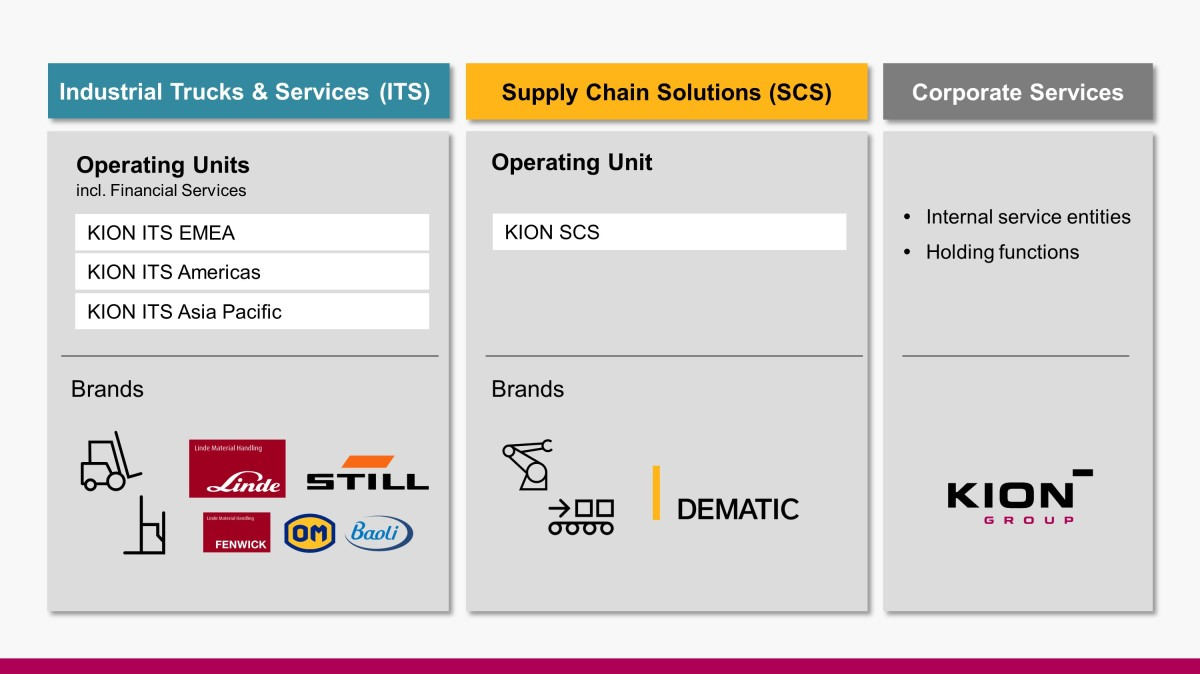
\includegraphics[width=5in]{images/Chap0/KION_Segments.jpg}\\
    \caption{KION segment services and companies \cite{R1}}
    \label{KION Segments}
    \end{center}
    \end{figure}

    
\subsection{KION Management Hierarchy}

The company is composed of departments managing the operations in all companies that are divided by scope of 
interest like R\&D, Management, finances, etc.. Figure \ref{KION Hierarchy} illustrates the different areas of 
responsibility of the Executive
Board. The Autonomous vehicles team belongs to the Mobile Automation department under CTO. 

\subsection{STILL Products}

The 2017-established Autonomous vehicles team aims to develop fully automated solutions that leverage 
novel technologies to create innovative services delivered through forklift trucks. 
The vehicles are developed while keeping safety and high-performance as the main priorities.  

iGo neo shown in Figure \ref{iGoNeo} is one of the main products developed by the department, it is a low level order picker transformed 
into the agent's autonomous assistant. Functioning in autonomous or semi-autonomous modes, it can follow 
the operator and their pace while avoiding obstacles and perceiving their surroundings as well as pick 
and place pallets in designed areas. Its added value is in preserving ergonomics of the operators by 
preventing heavy load carrying for long distances and decreasing the driving ascents and descents by 75\% 
thus increasing the personal and collective performances \cite{R3}.

\begin{figure}[H]
    \begin{center}
     % Requires \usepackage{graphicx}
    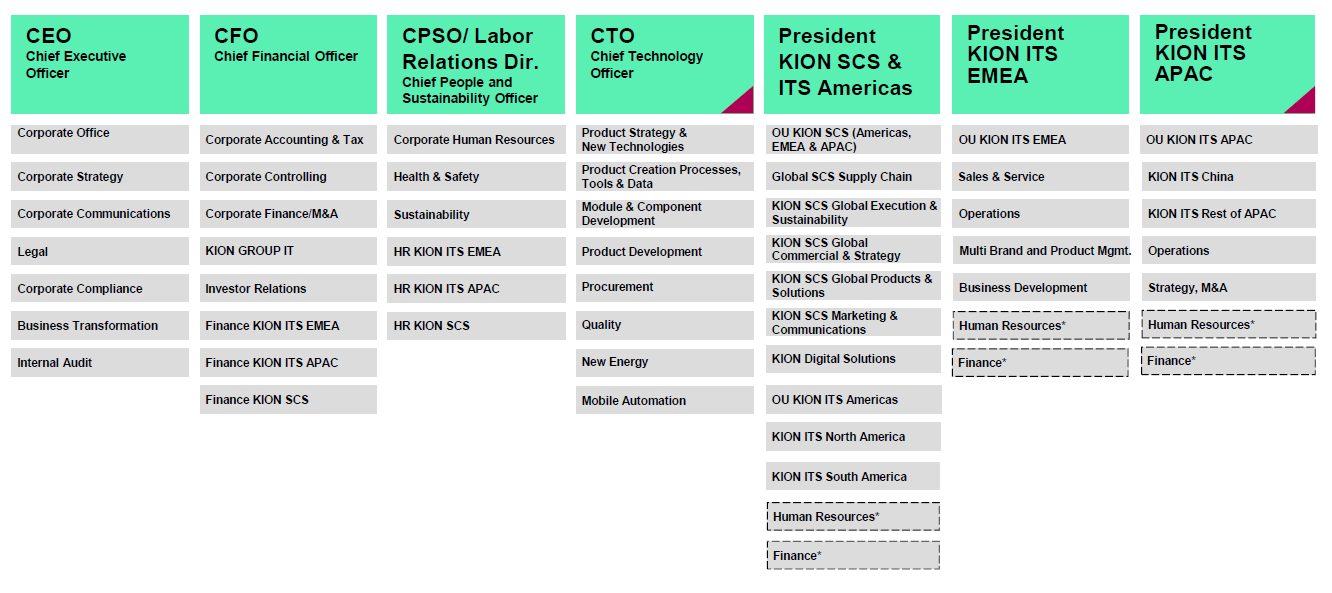
\includegraphics[width=\linewidth]{images/Chap0/KION_Hierarchy.png}\\
    \caption{KION Executive Board responsibilities as of 01.2024 \cite{R2}}
    \label{KION Hierarchy}
    \end{center}
    \end{figure}

As STILL specializes in forklift trucks, it counts many other products. Trucks are either Diesel or 
Gas fueled, or electric trucks that use Li-Ion batteries. Depending on the client's warehouse type, they can
choose from a vast range of reach trucks Figure \ref{Reach trucks}, hand pallet trucks Figure \Ref{hand truck}, 
double stacker trucks Figure \Ref{double-}, and Automated industrial Trucks Figure \Ref{iGoNeo} \cite{R4}.
A small selection of the vast range of STILL products is presented here. 
Automation can be applied to driver-requiring trucks to fully automate them.


\begin{figure}[h!]
    \centering
    \begin{minipage}{0.45\textwidth}
        \centering
        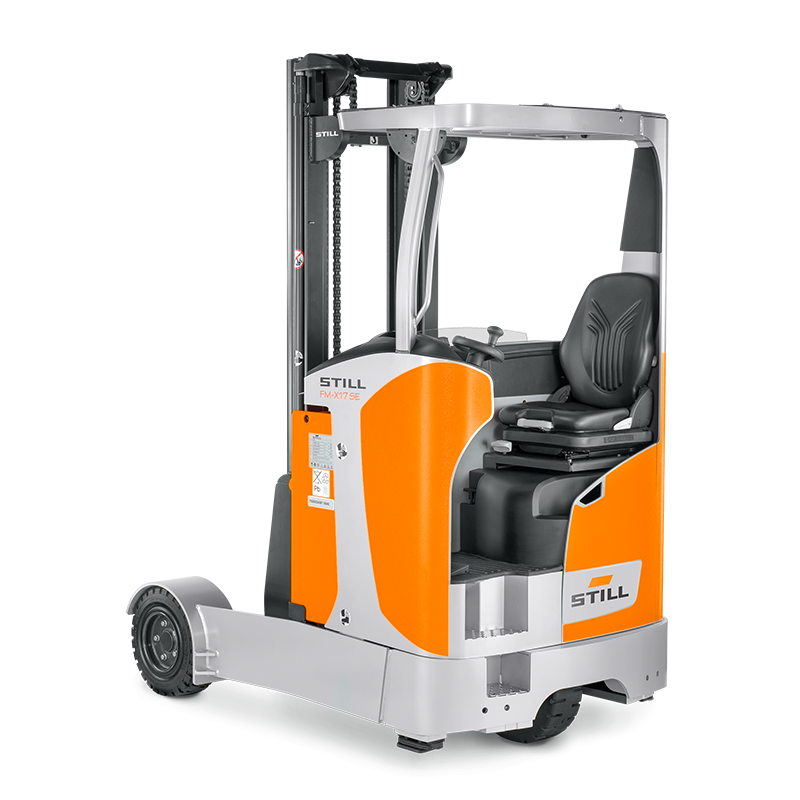
\includegraphics[width=\linewidth]{images/Chap0/Reach trucks.png} % Replace with your figure
        \caption{STILL reach truck}
        \label{Reach trucks}
    \end{minipage}
    \begin{minipage}{0.45\textwidth}
        \centering
        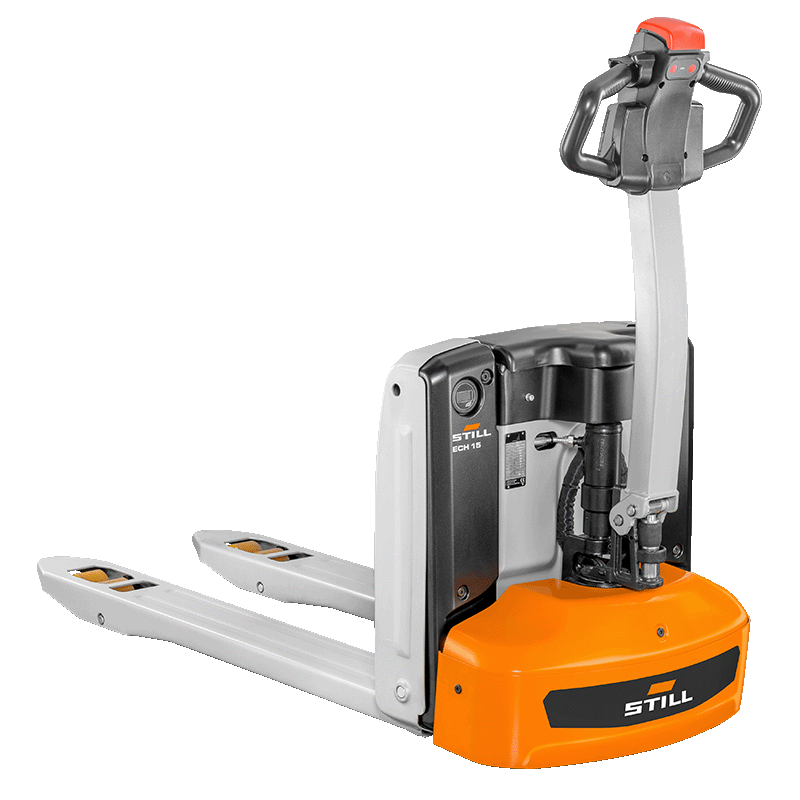
\includegraphics[width=\linewidth]{images/Chap0/hand truck.png} % Replace with your figure
        \caption{STILL hand truck}
        \label{hand truck}
    \end{minipage}
\end{figure}

\begin{figure}[H]
    \centering
    \begin{minipage}{0.45\textwidth}
        \centering
        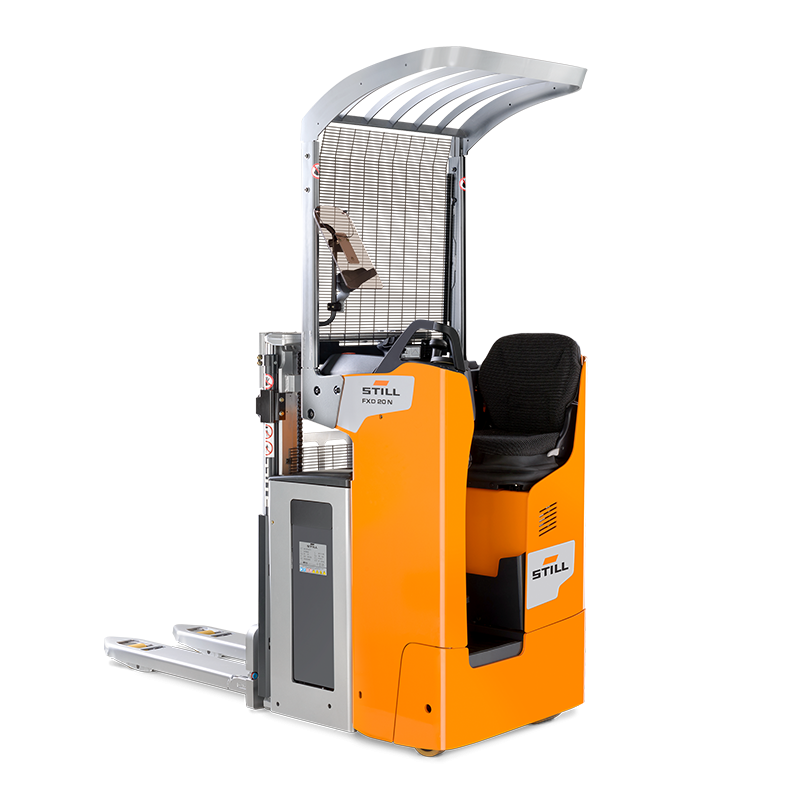
\includegraphics[width=\linewidth]{images/Chap0/double-.png} % Replace with your figure
        \caption{STILL rider truck}
        \label{double-}
    \end{minipage}
    \begin{minipage}{0.45\textwidth}
        \centering
        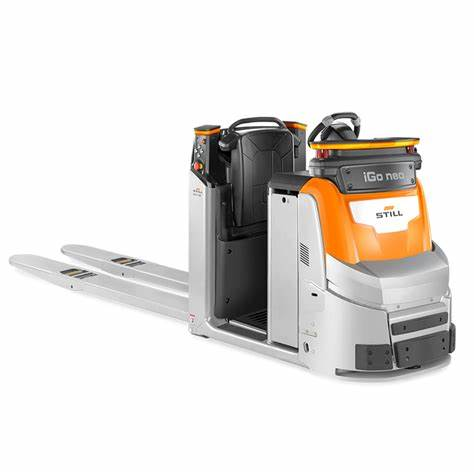
\includegraphics[width=\linewidth]{images/Chap0/iGoNeo.jpg} % Replace with your figure
        \caption{STILL Autonomous order picker}
        \label{iGoNeo}
    \end{minipage}
\end{figure}

Despite the impressive capabilities of the iGo neo and similar autonomous vehicles, the implementation 
of such advanced technology brings up several challenges, particularly in ensuring reliable and predictable 
behavior under all operating conditions. This leads to a key motivation for further investigation and improvement 
in the field.
The next section focuses on the process followed during the development of the project. 



\section{Work Structure and Methodology}

Our team adopts an Agile Scrum methodology showcased in Figure \Ref{Agile Scrum Process} to ensure 
efficient and flexible project management. Here’s how we approach our work:

\begin{figure}[H]
    \begin{center}
       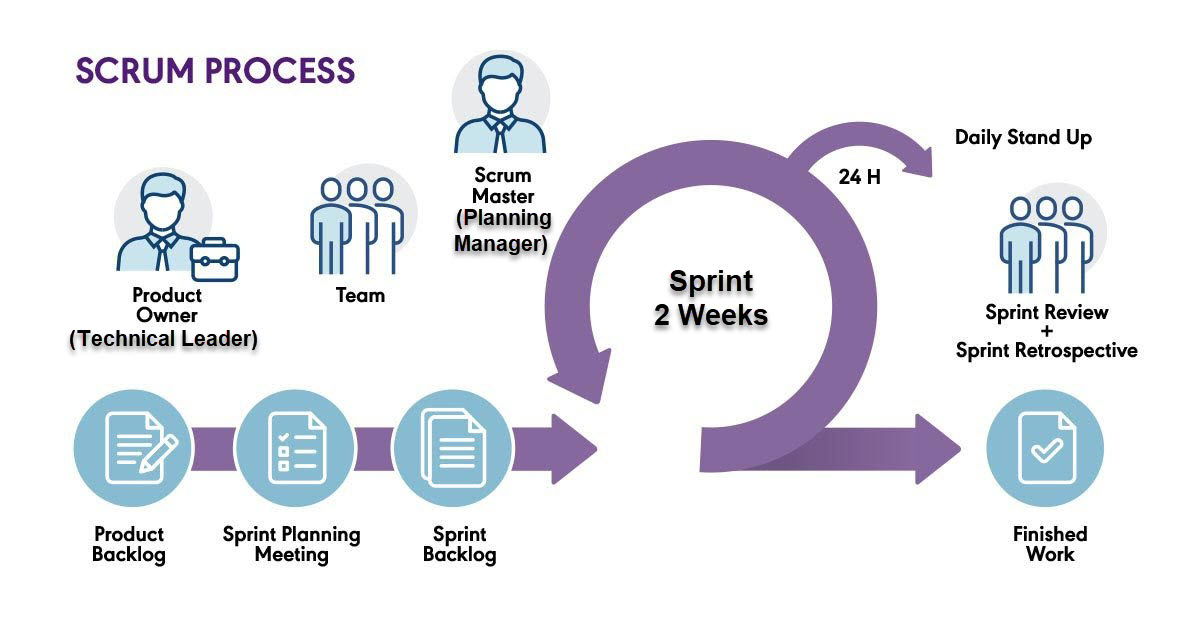
\includegraphics[width=6in]{images/Chap0/blog-scrum-process-opt.jpg}\\
       \caption{Agile Scrum Process \cite{R6}}
       \label{Agile Scrum Process}
       \end{center}
\end{figure}

\subsection{Agile Scrum Framework} 
To follow the Agile Scrum framework 4 main tools/ are used:
\begin{itemize}
    \item \textbf{Jira: } We use Jira to organize and track our tasks and progress. Jira allows us to create 
    and manage tickets, which are detailed records of tasks, bugs, or features that need attention. 
    Each ticket is assigned to team members and tracked through its development stages until completion.

    \item \textbf{Sprints: } Our work is organized into 2-week sprints. Each sprint is a focused period 
    where we aim to complete a set of predefined tasks. At the start of each sprint, we hold a meeting to 
    review the previous sprint: every team member presents their completed tickets, and communicates the 
    changes or blockers that appeared during the process and plan for the next sprint: decide which tasks 
    will be tackled during the sprint. 
    This helps us maintain a steady pace and regularly deliver increments of our project.

    \item  \textbf{PI Planning: } Every quarter, we engage in Program Increment (PI) planning with the 
    mobile automation teams. The PI happens in two phases: each team prepares their planning for the next 3
    months, then it is discussed and tailored again in a bigger round. This planning session helps us align 
    our goals and strategies for the upcoming quarter. We review progress, set objectives, and coordinate 
    with other teams to ensure that our work is aligned with broader project goals and company vision.

    \item \textbf{Daily Standups: } We hold 15 minutes long daily standup meetings to keep everyone on the 
    same page. During these meetings, team members share updates on their progress, discuss any challenges 
    they are facing, and outline their plans for the day. This practice promotes transparency, communication and quick 
    problem-solving through collaboration.

\end{itemize}

\subsection{Version Management}
For Version Management, the team collaborates over \textbf{GitHub: }We use GitHub for version control and 
code management. GitHub allows us to 
    collaborate on code, track changes, and manage different versions of our project. Each team member 
    can contribute to the codebase, and we use pull requests to review and integrate new features.


\subsection{Communication and Collaboration}
For daily communication and effective organization, the following tools are put to use:
\begin{itemize}
\item  \textbf{Microsoft Teams: }We use Microsoft Teams for real-time communication and collaboration. 
Teams provides a platform for chatting, video calls, and sharing files, facilitating smooth and efficient 
interactions among team members.

\item  \textbf{Microsoft Outlook: }Outlook is used for email communication and scheduling. It helps us 
manage meetings, track important messages, and coordinate tasks and deadlines.
\end{itemize}

\subsection{Project Timeline}

By integrating these tools and practices, we ensure a structured yet flexible workflow, enabling us to adapt 
to changes, communicate effectively, and deliver high-quality results.


\section{Graduation project Motivation and Problem Statement}

\subsection{Motivation}


While autonomous vehicles can be highly reliable and efficient in carrying out various 
tasks, their behavior is not always predictable or easily explained. The output often 
exhibits a stochastic nature. For example, an obstacle-avoiding solution planned by 
the autonomous vehicle may be safe and correct but might follow an unusually shaped path. 

Such stochastic behaviors can lead to a lack of trust and interest in robotized forklift 
trucks from a customer’s perspective. This unpredictability can cause customers to 
question the system's repeatability, fearing that it may not perform consistently in 
critical situations. Moreover, the unexpected nature of these behaviors can make it 
difficult for operators to understand and anticipate the vehicle's actions, further 
reducing confidence. 

Adding to these concerns, many autonomous systems, particularly in the intralogistics 
sector, require significant commissioning efforts before they can be implemented in 
a new environment and begin their service. Whether it's a required software integration, 
sensors installations, or 
measurements, these systems demand substantial time, information and financial investment—three 
crucial resources that STILL aims to optimize. Innovation in automation should involve 
the development of optimal solutions that are easy to 
commission in a new environment. These so-called "plug-and-play" solutions reduce 
the effort required and allow customers to start benefiting from the autonomous 
features with just the physical truck on-site and available information about the 
warehouse. the rest, is online recognition and processing. This approach 
significantly enhances the impact and convenience of the technology. 

The autonomous vehicles department focuses on creating reliable, efficient, and 
explainable systems to build trust with customers, encouraging adoption of the technology. 
With a focus on explainable AI, the technology becomes more interpretable, helping customers 
understand decision-making processes and increasing their confidence in its safety and reliability.

\subsection{Problem statement}

Autonomous navigation is a topic where explainable intelligence can be integrated. 
Robotic forklifts execute missions such as transporting pallets from one place to another: 
picking up or dropping pallets.
A typical mission is splitted into:
\begin{itemize}
    \item a movement to a source
    \item a pickup
    \item a movement to the destination
    \item a drop
\end{itemize}
The movement to the source or the destination is exemplified by figure \Ref{move} where 
\(station1\) is considered the source station that the truck is headed to.
However, the truck arrives at a distant pose from the shelf or pallet,
the distance is clearly seen in figure \Ref{dock}. In addition, its forks are facing the 
wrong direction because driving the truck should happen like the arrow shows on figure \Ref{move} 
to avoid hitting humans or materials with the forks.
The distance is intended because the truck needs a maneuver to make its forks dock (enter) the shelf
as they are the part that picks up or drops the pallet.
This work focuses on the subtask of an autonoumous online linking of the vehicle to the shelf
independantly from the task to be performed (pick up/drop). 

The path that involves this maneuver is called the "link path" that guides the truck to the pallet or the drop 
pose which is the shelf inside the station as illustrates figure \Ref{dock}. Online linking of the robotic 
forklift to the goal pallet or location takes place inside
the station. Online linking is mandatory because warehouse areas are subject to constant changes for instance,
shelves can be shifted from their expected
position and dynamic obstacles can show up, but, the vehicle needs precise recognition of the coordinates 
that it will reach. 
Precise recognition allows for correctness of the picking or dropping processes, otherwise, 
the task can fail. Furthermore, the vehicle has to account for the new obstacles and clutter inside 
of the station and avoid collisioning with them when driving to the destination shelf.

When it arrives at the station, the vehicle is fronted by these constraints:
%TODO: check these
\begin{itemize}
    \item The vehicle’s forks are not facing the destination shelf as shown in figure \Ref{dock} 
    but rather the opposite direction, 
    so a driving direction change is needed. 

    \item The vehicle is bulky in volume and mass (1200 to 4000 kg) with an overall 
    length of 2500 to 4000 mm  \cite{R5}
    which makes it challenging  to change directions: turning on the spot or 
    navigating in highly curved paths. 
    
    \item The pallet docking process has to be very precise to avoid shifts and mistakes. 
\end{itemize}


Figure \Ref{move} is a section of the model of a real warehouse. In this work,
the interest is around the following items of the model:
\begin{itemize}
    \item Dark Blue outline: walls of the warehouse
    \item Yellow Rectancles marked as stations: Warehouse stations: Actions like picking up or 
    dropping are performed in specific locations inside the warehouse called 
    stations, examples of which are named \(station1\), \(station2\), and \(station3\) on the figure \Ref{move}.
    Each station is designed to support specific warehouse functions and their general mission
    is to facilitate and organize material handling operations. 
    Each station contains a \textbf{shelf} that contains the pallets to be picked or dropped. 
    \item Black rectangles: storage shelves (also called racks), where the  pallets and material are 
    stored. 
    \item Turquoise blue lines: Global paths that connect the stations.
    The truck takes these routes when navigating from a station to the other while avoiding 
    obstacles online if they occur.
    \item Gray rectangles are starting position of the truck around the warehouse. For instance,
    the truck can be placed at these positions before starting its autonomous navigation and 
    task fulfillment.

\end{itemize}

\begin{figure}[H]
    \begin{center}
       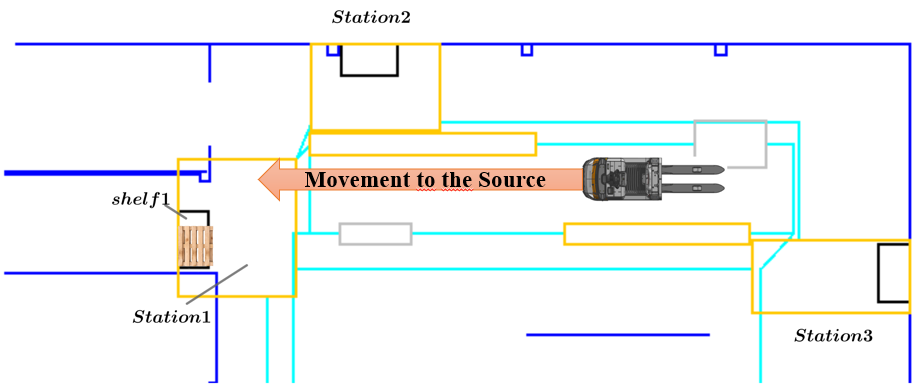
\includegraphics[width=5in]{images/Chap0/move.png}\\
       \caption{Vehicle Moving towards station 1}
       \label{move}
       \end{center}
\end{figure}

\begin{figure}[H]
    \begin{center}
       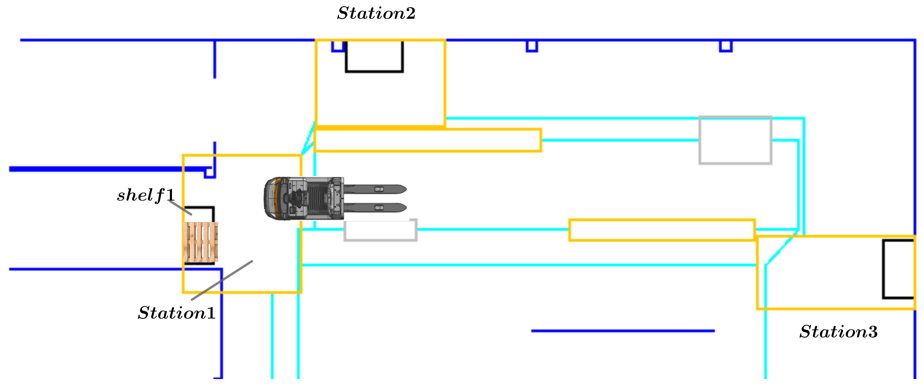
\includegraphics[width=5in]{images/Chap0/arrive.png}\\
       \caption{Vehicle arrives at station 1 and ready to execute the task}
       \label{dock}
       \end{center}
\end{figure}

To summarize, the goal is to autonomously and optimally transport the vehicle from the position of entering the station in
figure \Ref{dock_wait} to the position of docking the shelf in figure \Ref{dock_done} while accounting for obstacles,
kinematics of the vehicle, and maximizing speed. 

\begin{figure}[H]
    \begin{center}
        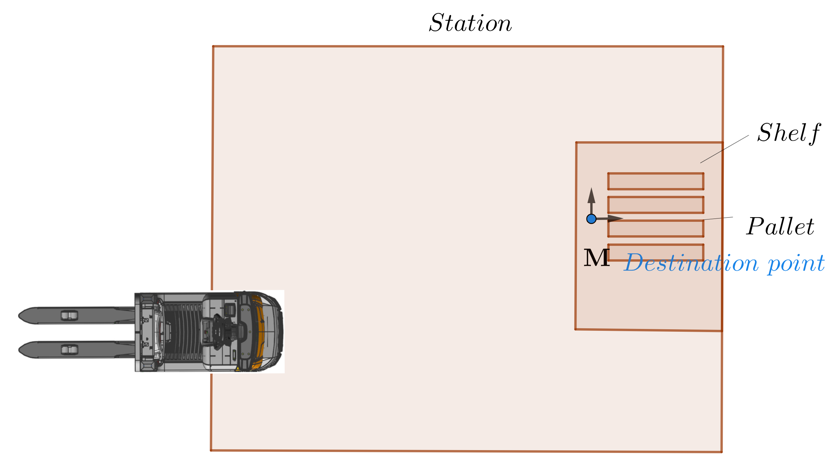
\includegraphics[width=4in]{images/Chap0/dock_wait.png}
        \caption{Vehicle entered the station waiting for docking the shelf}
        \label{dock_wait}
       \end{center}
\end{figure}
\begin{figure}[H]
    \begin{center}
        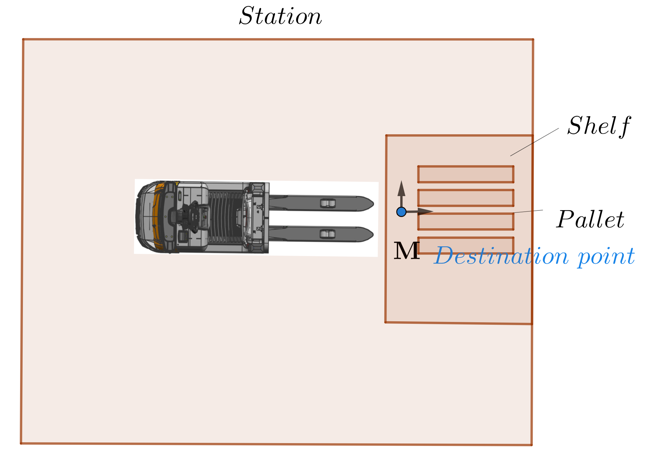
\includegraphics[width=4in]{images/Chap0/dock_done.png}
        \caption{Vehicle docked the shelf}
        \label{dock_done}
       \end{center}
\end{figure}

The next chapters lead to the available approaches, the goals to be fulfilled, and the methodology to adress
the problem statement.


\section*{Conclusion}
This chapter introduced the host company, STILL GmbH, and its role within the KION Group, highlighting its 
management structure and product offerings. It also outlined the motivation behind the graduation project 
and the specific problem statement it aims to address. The chapter provided an overview of the work structure 
and methodology, focusing on the Agile Scrum framework and key tools for version management. Additionally, 
the importance of effective communication and collaboration throughout the project was emphasized. These 
foundational elements set the stage for the detailed work in subsequent chapters.
\part*{Chapter 2 \\State of the Art}
\chapter{State of the Art: Optimal path planning for autonomous robots}

\renewcommand{\chaptername}{Chapter}

\section*{Introduction}
This chapter focuses on a sythesis of the literature around Optimal Near-field Path planning
for robots in Intralogistics environments. 
It starts with an explanation of the fundamental aspects this work is based on 
as Automated Mobile Robots (AMRs), Near-field Path planning and Optimization techniques 
with a focus on Intralogistics.
Then it focuses on the path planning approaches proposed to rise to the existing challenges.
Later, the topic of optimization is outlined, investigating the decision-making science
that leads to the elimination of some path planning drawbacks.
It concludes with a discussion around which works from the literature can be used for this problem 
statement and how they can be exploited for this work.

\section{Intralogistics Environments}
Intralogistics refers to the management, control, and optimization of internal material and 
information flow within a warehouse \Ref{R28}. It encompasses all physical and operational processes 
involved in the movement of materials and goods. This concept was introduced and defined by 
the German Engineering Association (VDMA). Figure \Ref{Areas} covers various aspects of 
intralogistics areas, including 
the storage, transportation, supply, Manufacturing, and disposal of production materials, as well as 
shipping. 
The scope of this work is focused around the warehouse 
area where storage: picking, and placing, takes place. 
In brownfield applications, introduced in the General Introduction, the warehouse environment is 
usually a crowded and cluttered 
atmosphere: The nature of activities like manufacturing storing installs a high level of 
dynamics, whether it is operators or other vehicles, and obstacles as boxes and pallets. 
The cluttered 
and highly dynamic nature of this environment makes it challenging to successfully 
implement robotic based solutions.

\begin{figure}[H]
    \begin{center}
        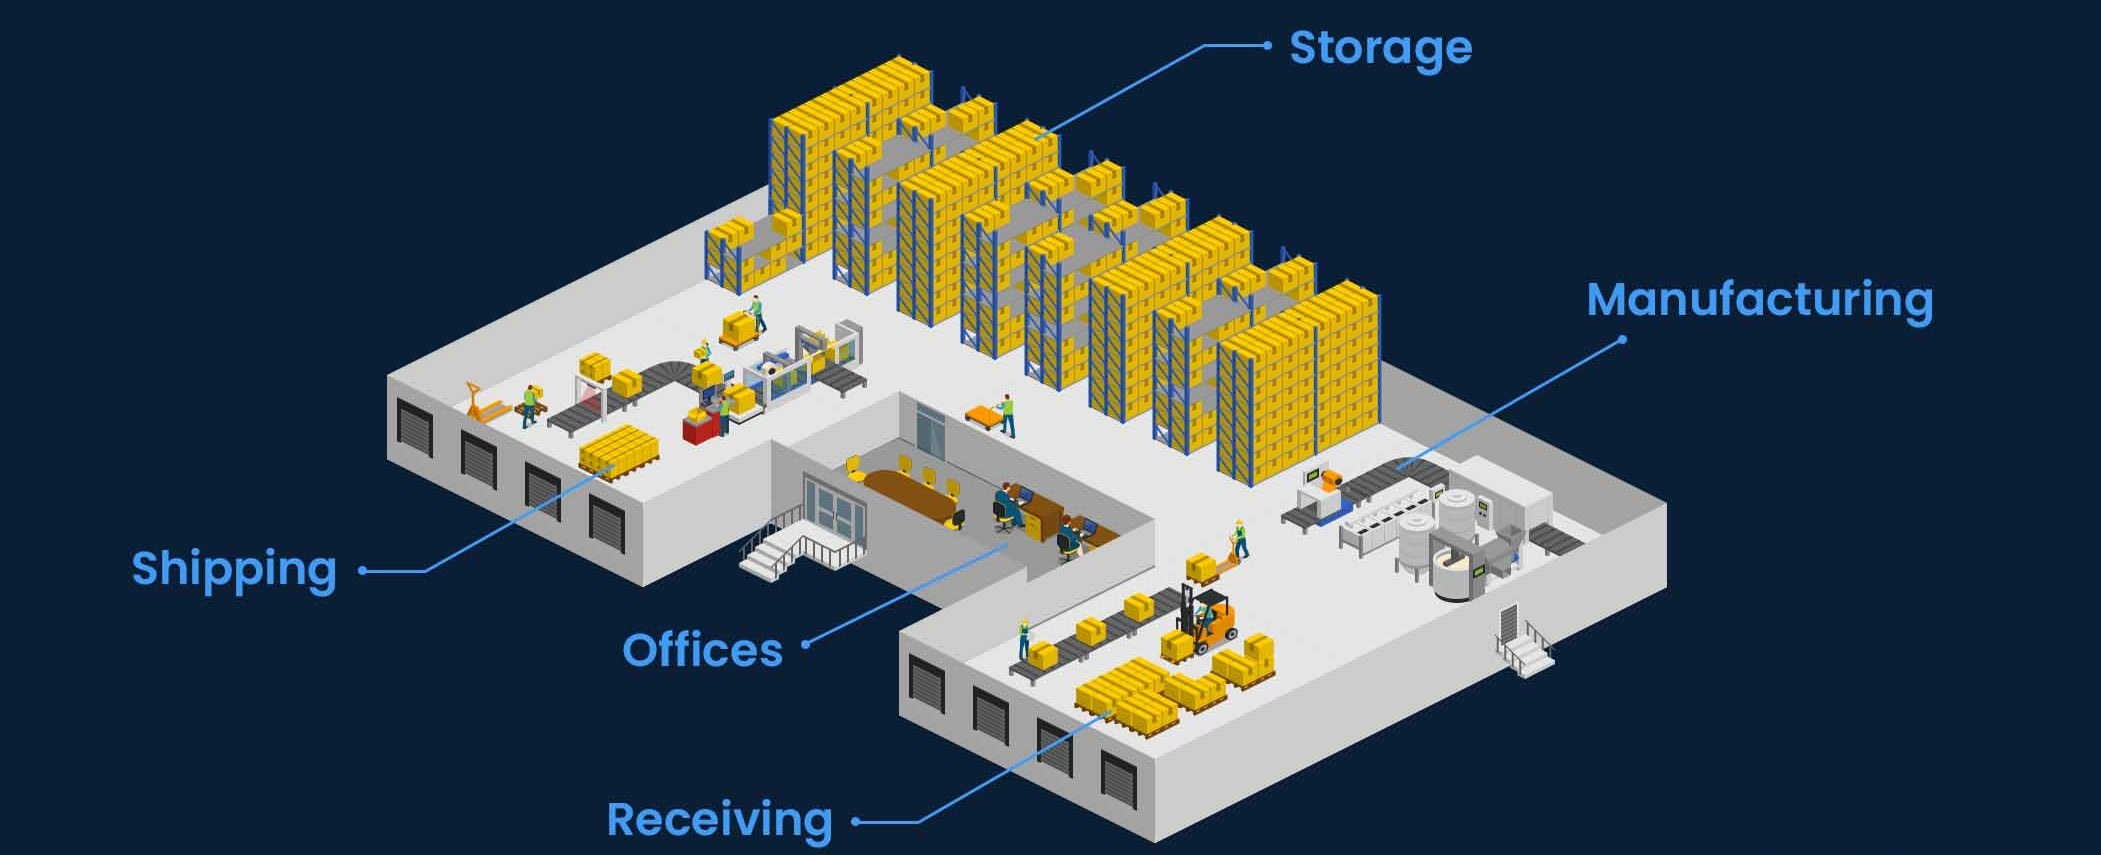
\includegraphics[width=6in]{images/Chap1/common-warehouse-areas.jpg}\\
        \caption{Common Intralogistics Environment Areas \cite{R46}}
        \label{Areas}
        \end{center}
\end{figure}

\section{AMRs in Intralogistics Environments}
Autonomous Mobile Robots (AMRs) are advanced robots designed to navigate and perform tasks independently 
in dynamic environments without the need for fixed infrastructure or human intervention. Equipped with 
sensors, cameras, and advanced software, AMRs can move around facilities like warehouses and 
factories, adjusting their paths based on real-time conditions. They are commonly used 
for material handling and transporting goods \cite{R7}.

AMRs are a type of non-holonomic vehicles. Non-holonomic vehicles are systems whose movement is subject 
to constraints that limit their ability to move freely in all directions. Specifically, their constraints 
depend on their configuration and velocities, meaning they cannot instantaneously move in certain directions 
(e.g., sideways), but must follow a specific path or series of movements to achieve certain positions. 
This contrasts with holonomic systems, which can move in any direction directly without such constraints \cite{R28}.

In the Intralogistics field, AMRs were introduced as a revolution to Automated Guided Vehicles (AGVs) \cite{R7}. 
First introduced in 1955, AGVs performed tasks like 
material handling. AGVs are managed by top-level software that handles task planning, 
providing the vehicles with intermediate waypoints to navigate from start to end points \cite{R7}.
On the other hand, AMRs are automated in a way that makes them find the solution to unexpected problems, 
in fact:
Figure \Ref{AMR-VS-AGV}, shows the difference in behavior between an AMR and an AGV in the case of a 
new obstacle. While AMRs are able to surpass the obstacle through sensors recognition and obstacle 
avoidance algorithms, AGVs require human intervention to eliminate the obstacle before restarting the navigation.

AMRs fit in the cluttered ares of warehouses. Their perception of the surrounding information allows for
low commissioning efforts: they are able to localize themselves, plan then navigate to the goal and reach their 
destinations autonomously. Their operation does not require an expert or an engineer's intervention which 
limits the commissioning and utilization costs.

\begin{figure}[H]
    \begin{center}
       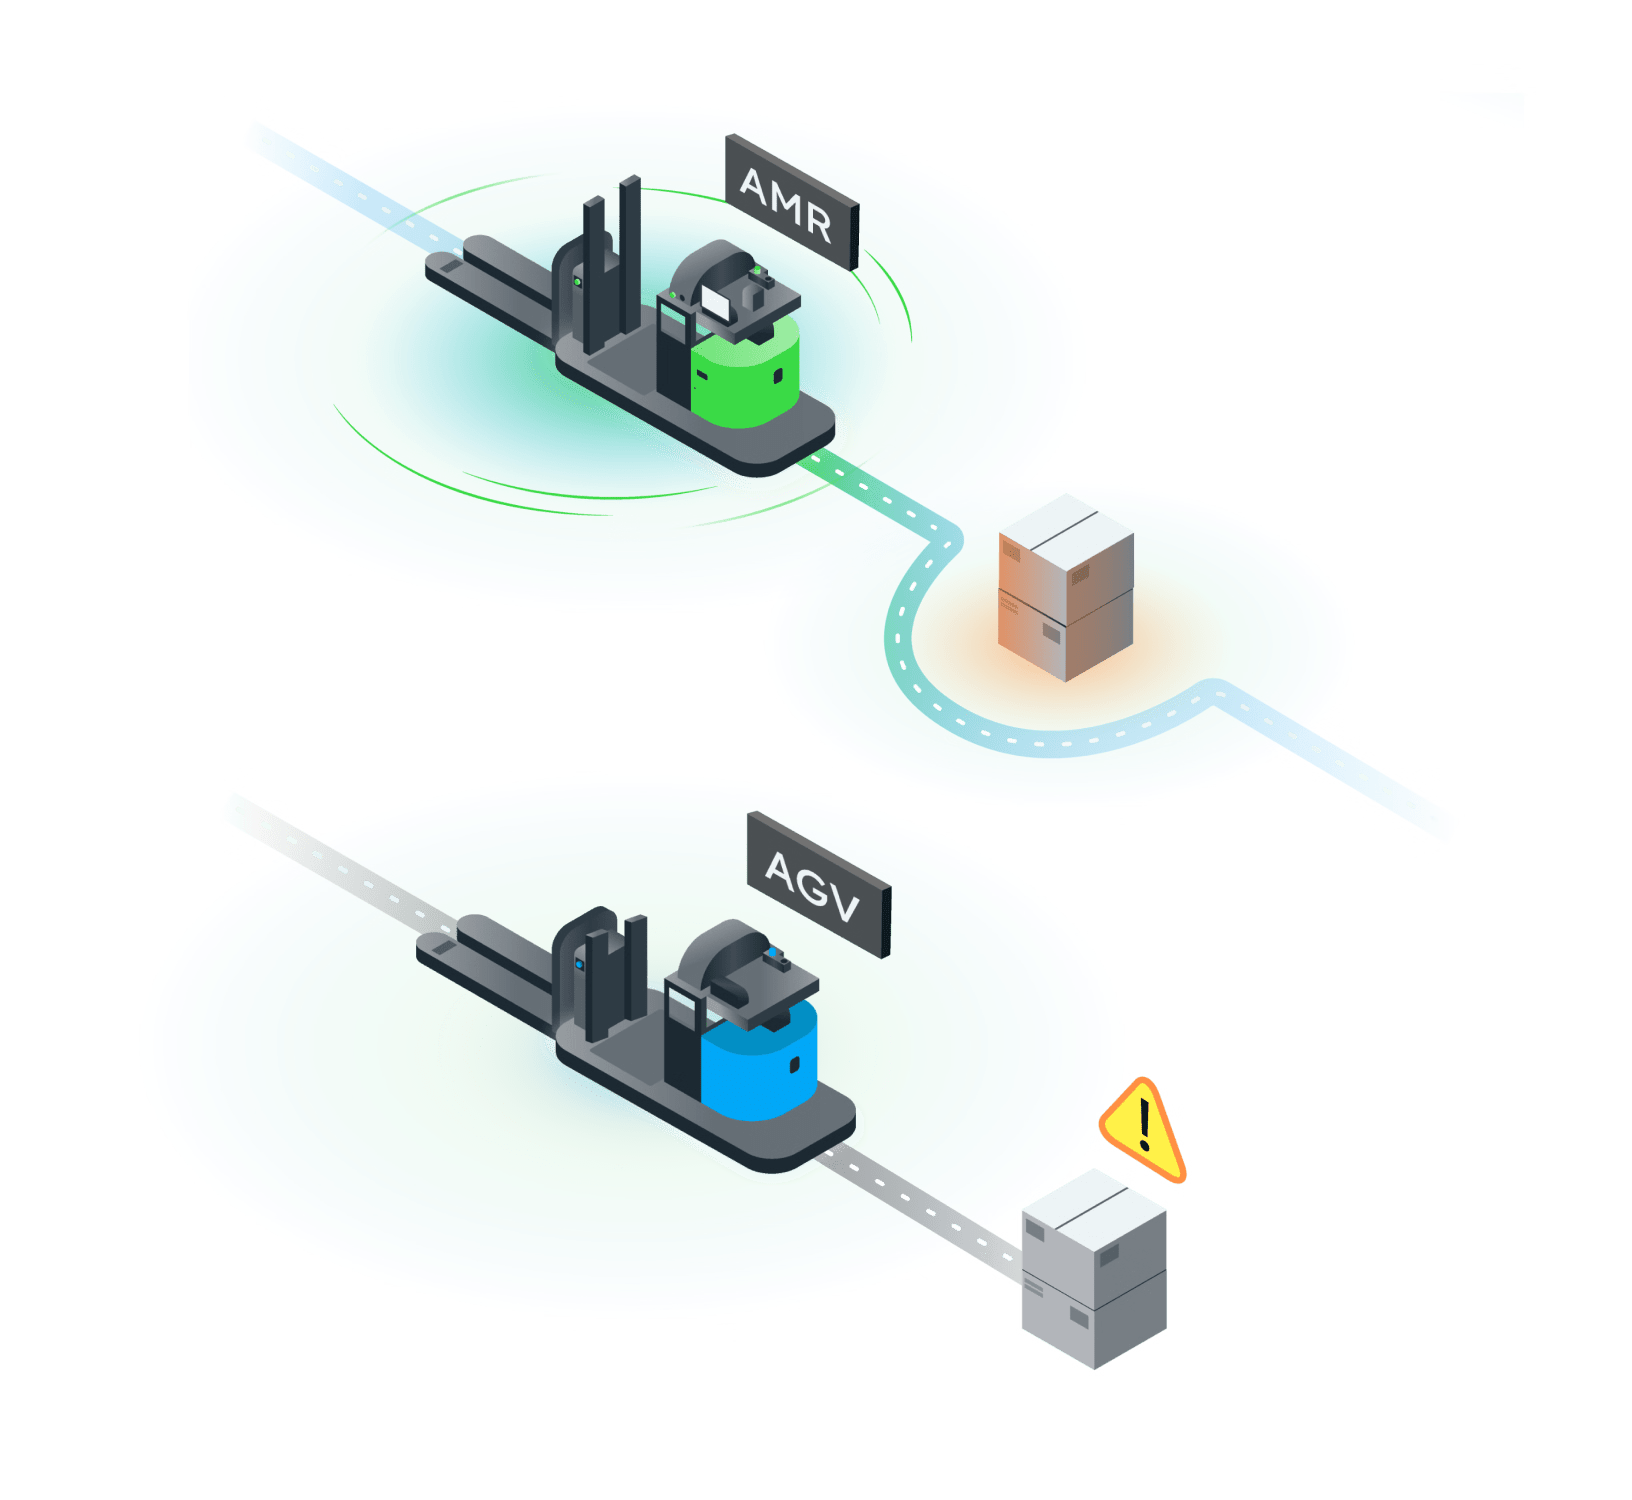
\includegraphics[width=4in]{images/Chap1/AMR-VS-AGV.png}\\
       \caption{AMR and AGV behaviors at presence of an obstacle \cite{R9}}
       \label{AMR-VS-AGV}
       \end{center}
\end{figure}

%\begin{figure}[H]
%    \begin{center}
%       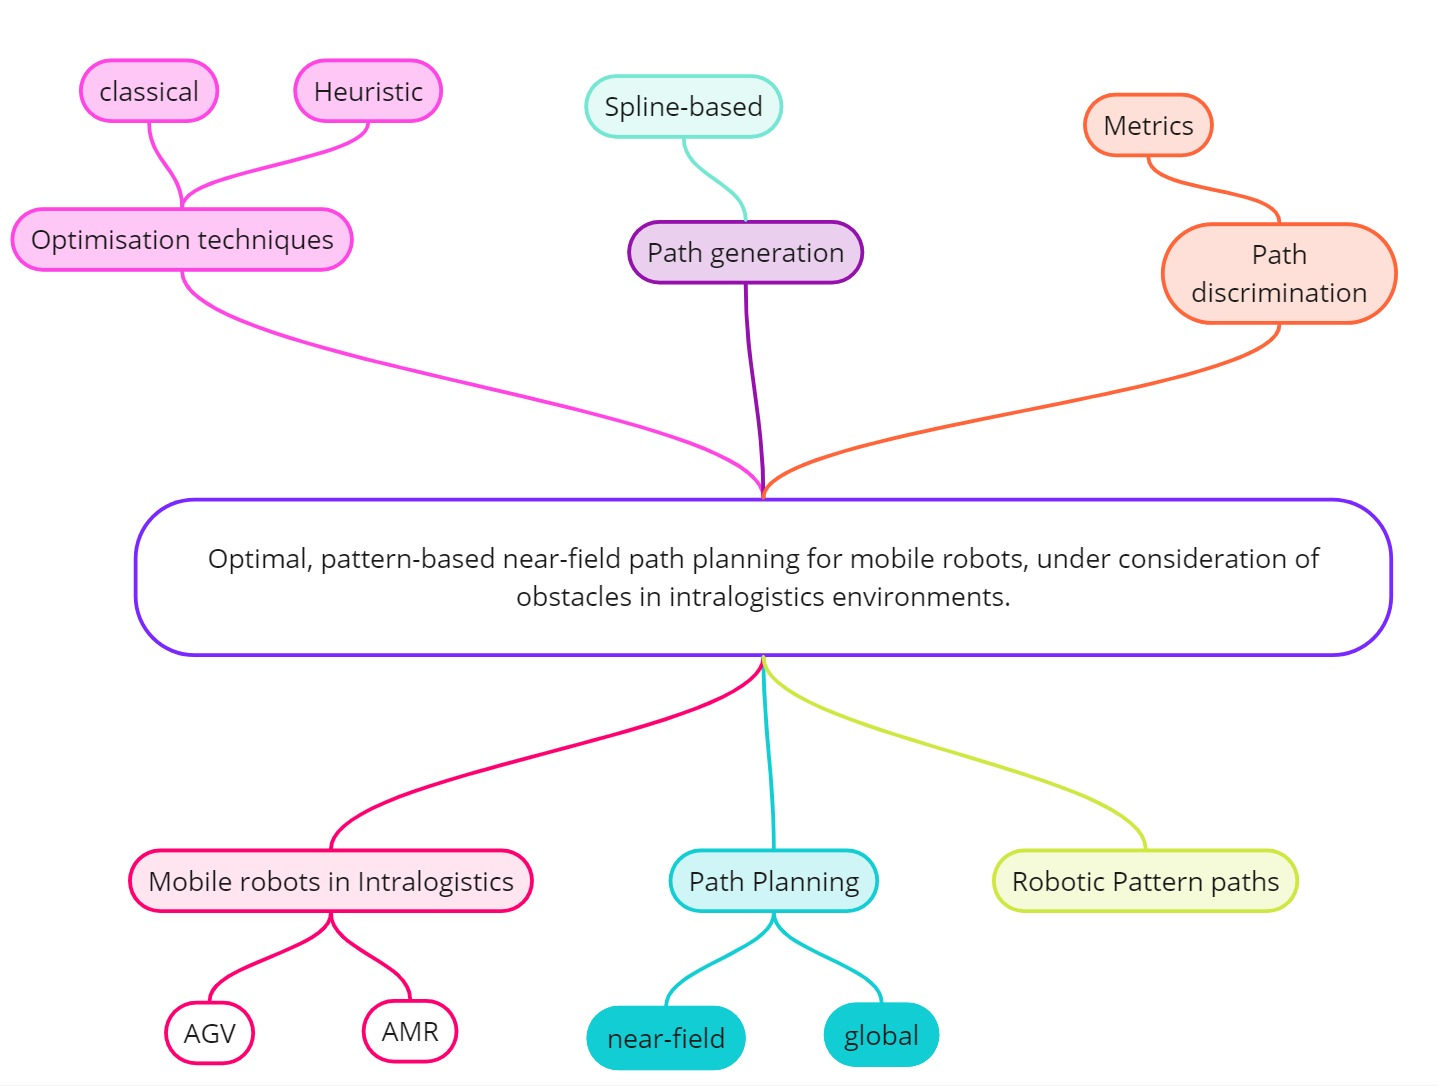
\includegraphics[width=5in]{images/Chap1/Fig1.jpg}\\
%       \caption{Mind map of the key topics}
%       \label{mindmap}
%       \end{center}
%\end{figure}

\section{Path Planning}
This section will dive into the path planning state of the art: outlining its promising 
opportunities and current challenges, detailing the different approaches, and discussing
%how to employ their efficienyćy for this 
their efficiency and compatibility with the problem statement.

\subsection{Path Planning for autonomous robots: Opportunities and challenges}
%opportunities
Path planning for mobile robots involves creating and generating efficient routes 
for the robot to travel from a starting position (A) to a target position (B), 
ensuring minimal time and travel distance while avoiding collisions with nearby objects \cite{R7}. Literature 
differentiates between two main types of path planning: 
global and local path planning \cite{R11}. Global planning involves finding an optimal path from 
the start to the target position based on sensor input within a known, static environment, 
whereas local planning focuses on real-time path planning and obstacle avoidance, typically used online while 
moving to avoid dynamic obstacles \cite{R11}.

In complex environments, movement and task fulfillment must be done carefully and accurately given 
the volume of the vehicle and the value of the handled material. With appropriate input from various sensors, 
such as laser 
scanners, cameras, and LiDAR providing robots can perceive of their surrounding environment and plan the right path
accordingly. This hardware innovation made navigation flexibility and autonomous recovery 
after failure possible\cite{R7}.
The relevance of efficient path planning, mainly in the intralogistics sector, is derived from the constant need 
of optimizing material flow, productivity rates, and cost-effectiveness. Path planning reduces
travel time and distances when moving goods and thus, improving overall operational costs by allowing robots 
to take the most optimal routes when moving goods. By minimizing unnecessary detours and avoiding congested areas, 
robots can complete tasks more quickly, leading to faster material handling cycles.
In those dynamic environments (see chapter 2, section 1), operators and employees are moving around, 
goods and pallets are 
being transported or stocked, and materials must be handled safely and carefully.
Flexibility in routing and planning, enables the AMRs to always drive the optimal path
based on the space settings. This flexibility offers several benefits, such as:

\begin{itemize}
    \item Independence from Human intervention if an unexpected situation raises 
    -AMRs do not require assistance, unlike AGVs \cite{R7}.
    \item Reduced energy consumption thanks to optimal, smooth and short paths that adhere to 
    the vehicles' kinematics, allocated task and travel time.
    \item Robustness and responsiveness thanks to decentralized decision-making: enables fast 
    recovery and change of strategy after failure\cite{R7}.
\end{itemize}

Efficient path planning is critical for ensuring safe and reliable handling of objects in dynamic environments. 
By maintaining safe distances from both static and moving obstacles, including people, and continuously detecting 
surroundings, robots can ensure safety at all times. An optimized path improves both the length and 
smoothness of travel, minimizing travel time and boosting productivity, as tasks are repeated frequently 
throughout the day. As a result, it enhances operational efficiency, contributing to overall system 
performance.

AMRs, as the name suggests, are 
standalone systems that must compile and process such input and generate, through algorithms, 
efficient paths. Path planning serves as the crucial 
link between the robot’s sensor input and its motion control \cite{R10}.


%challenges 
%Todo: add reference for 
More that 60 years have elapsed since "Shaky" the first wheeled robot was running it first tests
in Stanford University' labs. However, most of the robotic related topic are still being researched and improved.
Dealing with all the aspects and challenges that robotics comes with can be very intricate. One of the major 
topics posing challenges to researchers is path planning. 
In \cite{R20}, authors reviewed recent path planning approaches and challenges
in dynamic unkown environments. 
% safety
Saftey in path planning was the main concern for 29 \% of the reviewed studies. Navigating efficient 
paths while avoiding collisions is challenging to accomplish. Collision avoidance is tightly related to perception 
input through sensors, analysis and use of the data. While it may seem simple for the robots to correctly analyze 
and recognize the surrounding objects, in reality, detailed understanding is not possible \cite{R21}. Issues are 
related to the accuracy of the sensors and the robustness of the algorithms. 
It is expected from the robot to 
perceive of the obstacles just like humans do, recognizing 3d shapes, dimensions, depth, direction and velocity, 
but from the 
robot's perspective, it is only able to recognize the outer surface that reflects the sensor's luminous signals. As shown in
figure \Ref{scamSim}, the simulated robot (in gray) is surrounded by 3 obstacles (blue polygons).
While the obstacles are polygon-shaped, the perception of the robot is limited to the surfaces that 
it can scan and does not see the hidden depth beyond these surfaces.

\begin{figure}[H]
    \begin{center}
        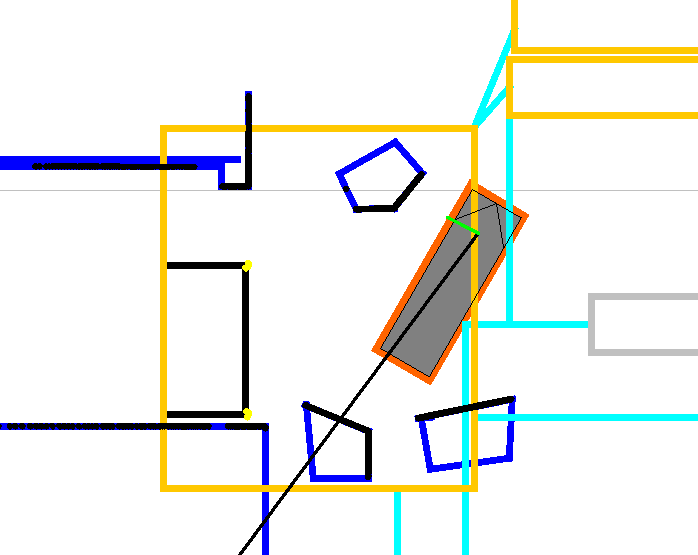
\includegraphics[width=4in]{images/Chap1/scan.png}\\
        \caption{
        Simulation of the robot's perception of surrounding obstacles.
        \newline \textbf{Yellow rectangle:} Station limits
        \newline \textbf{Black rectangle:} Shelf limits: where to pick or to place pallets
        \newline \textbf{In gray:} Robot in simulation
        \newline \textbf{Blue polygones:} Simulated obstacles
        \newline \textbf{Black lines:} Perceived obstacle points}
        \label{scamSim}
        \end{center}
\end{figure}

As a result, algorithms are to compensate the shadowed depth of obstacles by enforcing safety measures like 
keeping the vehicle at a safe distance from the obstacles and decelerating at the proximity 
of static and dynamic objects to avoid collisions \Ref{R28}.
In addition, this input contains noises caused by the sensors reflections of other objects
or inaccuracies \Ref{R28}. 
This makes it challenging to interpret the input and create deliberative systems as the built algorithms have to 
deal with the given data
in all cases and detect the inaccuracies and noises.
Beyond that, it is complex to generate feasible solutions in all types of environments,
some planners and algorithms risk stagnating in local minima and not converging to the optimal routes
due to the limited knowledge of the environment and the sensory limitations previously mentioned \Ref{R28}. 
Figure \Ref{local_minima} shows a simplified example of a potential wrong decision. A vehicle encounters two possible 
driving paths, similar to what might happen in a racking system. Based solely on sensor data 
(gray shaded area), the correct path cannot be determined. Only with global path planning (green path) 
can a long-term route be selected (black arrow), avoiding the risk of ending up in a dead end (red arrow). 
Assuming the global trajectory leads to the mission goal, any local deviations from this path should be 
kept minimal while avoiding obstacles.

\begin{figure}[H]
    \begin{center}
        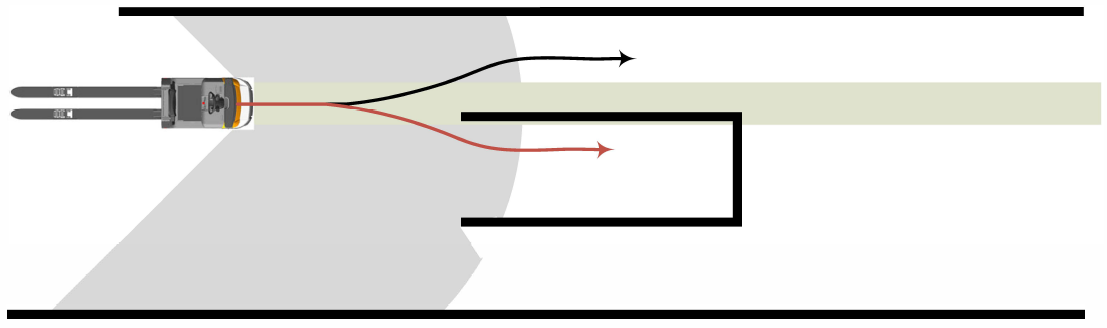
\includegraphics[width=4in]{images/Chap1/local_minima.png}\\
        \caption{Model of a local minima problem 
        due to limited sensor output \cite{R28}}
        \label{local_minima}
        \end{center}
\end{figure}

%Computational intensivity

Besides safety, computational cost is an interesting topic that researches 
are looking at. In a real time context, it is important to synchronize different tasks, 
analyze massive amounts of data generated by sensors and camera like point clouds and 2d/3d images, 
and compute the required decisions in a reliable and accurate way. As the complexity of the environment 
increases, so does the computational burden, often leading to longer processing times or the need for 
more powerful hardware \cite{R23}.

%smooth paths length and control:
While managing computational costs is crucial, it is equally important to ensure that the paths 
generated are not only computationally efficient but also smooth and short, as these factors 
significantly influence the robot's overall performance.
Given the kinematics of a robot, the destination's location and the clutter in the environment, 
path planners usually render rough paths. Cusps, which are sudden and sharp direction changes, and high
curvatures of the path are unusual path properties that are hard to drive, energy and time inefficient, 
and require continuous deceleration and accelerations. Long paths are also not favored. While they can be 
necessary to avoid obstacles or to create a smooth path, longer distances result in time consumption and 
extensive energy usage. 
Some path planner include post-smoothing methods that modify the paths after its creation and intervene by
shortening and smoothing paths areas while obstacles. In \cite{R23}, authors present approaches 
to implement post-smoothing methods like B-Splines, Shortcuts, Simplify Max, and vertex optimization. 
They conclude that different methods deal with certain 
improvements areas differently. For example, While Splines are outperformed in the curvature and cusps 
areas, they are efficient when it comes to path-smoothning computation time.  

In conclusion, tackling robot path planning requires looking at several improvement
areas: computational intensity, smoothing, and safety at the same time. Most path planning approaches 
are effective in the aspects that they focus on, but lack optimization in others. This further emphasizes that these 
challenges remain under research and are not yet fully addressed in the literature. While these challenges 
highlight areas needing further exploration, path planning approaches propose techniques 
to address them. Understanding these approaches can provide insights into potential solutions and 
advancements in overcoming the existing limitations.


\subsection{Near-Field Path Planning}
Path planning can be differentiated into Global Path Planning (GPP) and Local
Path Planning (LPP) or Near-Field Path Planning (NFPP). The GPP generates a global trajectory based on static and 
known environment model, such as the current pose, target location and the static components 
of the environment like shelves and walls \cite{R28}. 
The LPP generates relative trajectories and allows deviation from the previously generated global 
trajectory if disturbances in the travel path are detected. However, LPP tend to converge into local 
minima as explained in the previous section .

Due to the sheer number of publications around LPP, the work of  Kr\"uger-Basjmeleh \cite{R28} clusters 
processes into 4 groups. Figure \Ref{cluster} illustrates 4 clusters. 
The classification of the methods is done by dividing them into direction, speed, and path generating methods and 
other methods based on AI for NFPP. All methods rely equally on immediate sensory input from the 
environment as the basis for future tracking strategies.

\begin{figure}[H]
    \begin{center}
        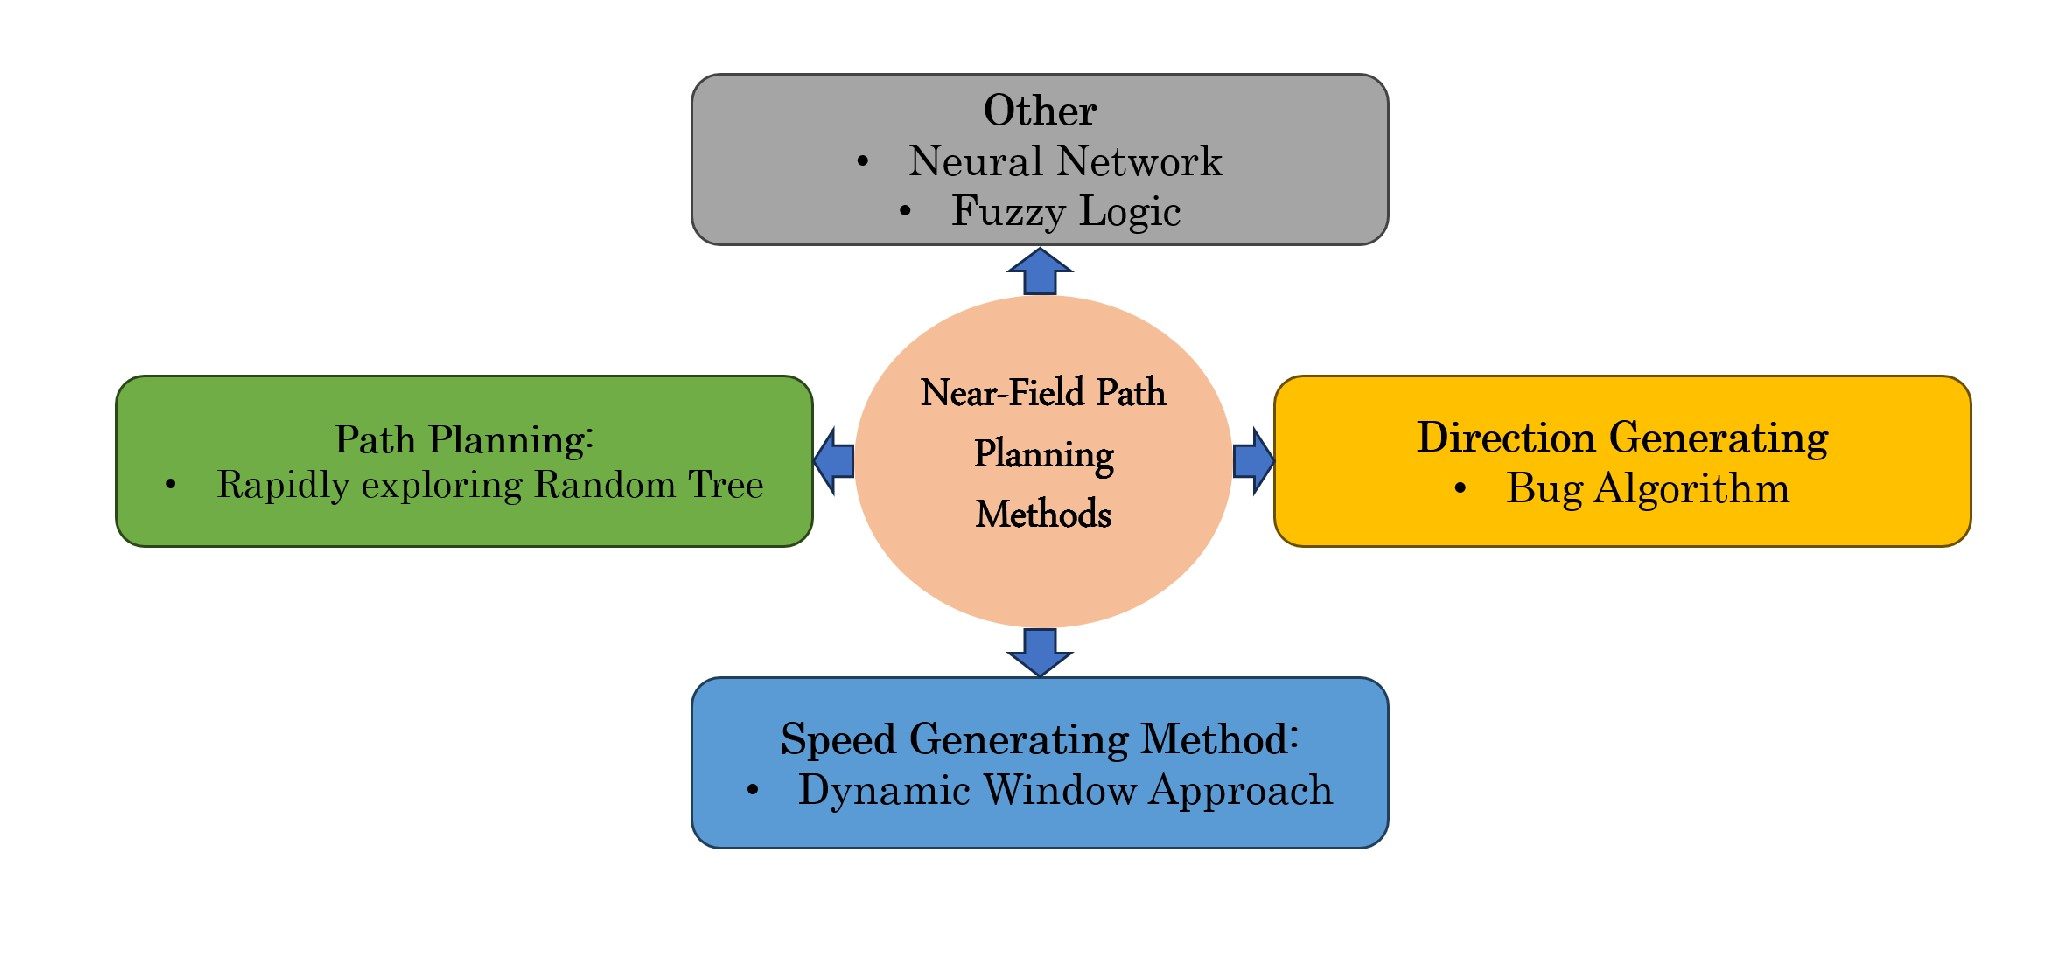
\includegraphics[width=6in]{images/Chap1/PP_Approaches.jpg}\\
        \caption{Clustering Of Near-Field Path Planning Approaches \cite{R28}}
        \label{cluster}
        \end{center}
\end{figure}

The process groups are then differentiated to identify their advantages, limitations and suitability 
to the problem statement. For each cluster one or two methods are studied and explained, through which 
the discrimination is made. 

\textbf{Direction-generating methods} compute feasible travel directions (directional state space) 
based on sensory input, which the AMR should follow in the next time step \cite{R28}.
A very simple algorithm for obstacle avoidance is the Bug algorithm.
In their research paper \cite{R25},
Buniyamin, N. et al. propose the point to point Bug algorithm to navigate in unknown environments. 
Bug algorithms are based on range sensors input. As illustrated by \ref{Bug_Algo}, the robot at the 
starting point (Start green dot), 
plans to move directly to the 
Goal (Goal Red dot). Then it rotates scanning for obstacle points. 
If it encounters a sudden obstacle point \((A)\), it navigates in its direction.
The robot rotates in the target's direction (\(B\) then \(C\)) until it is able to resume its direct path to 
the target based on the 
constant search for the shortest distance from the current standpoint or find the next obstacle. 

While this approach is simple from the computational point of view and the hardware used, it may not be 
optimal considering other metrics. First it can be significantly affected by sensory noises.
Besides, its path length optimality depends on the nature of the environments and the number of obstacles 
and its efficiency decreases if the complexity (obstacle density) of the test area increases: in figure 
\Ref{Bug_Algo}, the path rich in vertices : start-A, A-B, B-C, and C-goal, which makes it 
long and lacks optimization.

\begin{figure}[H]
    \begin{center}
        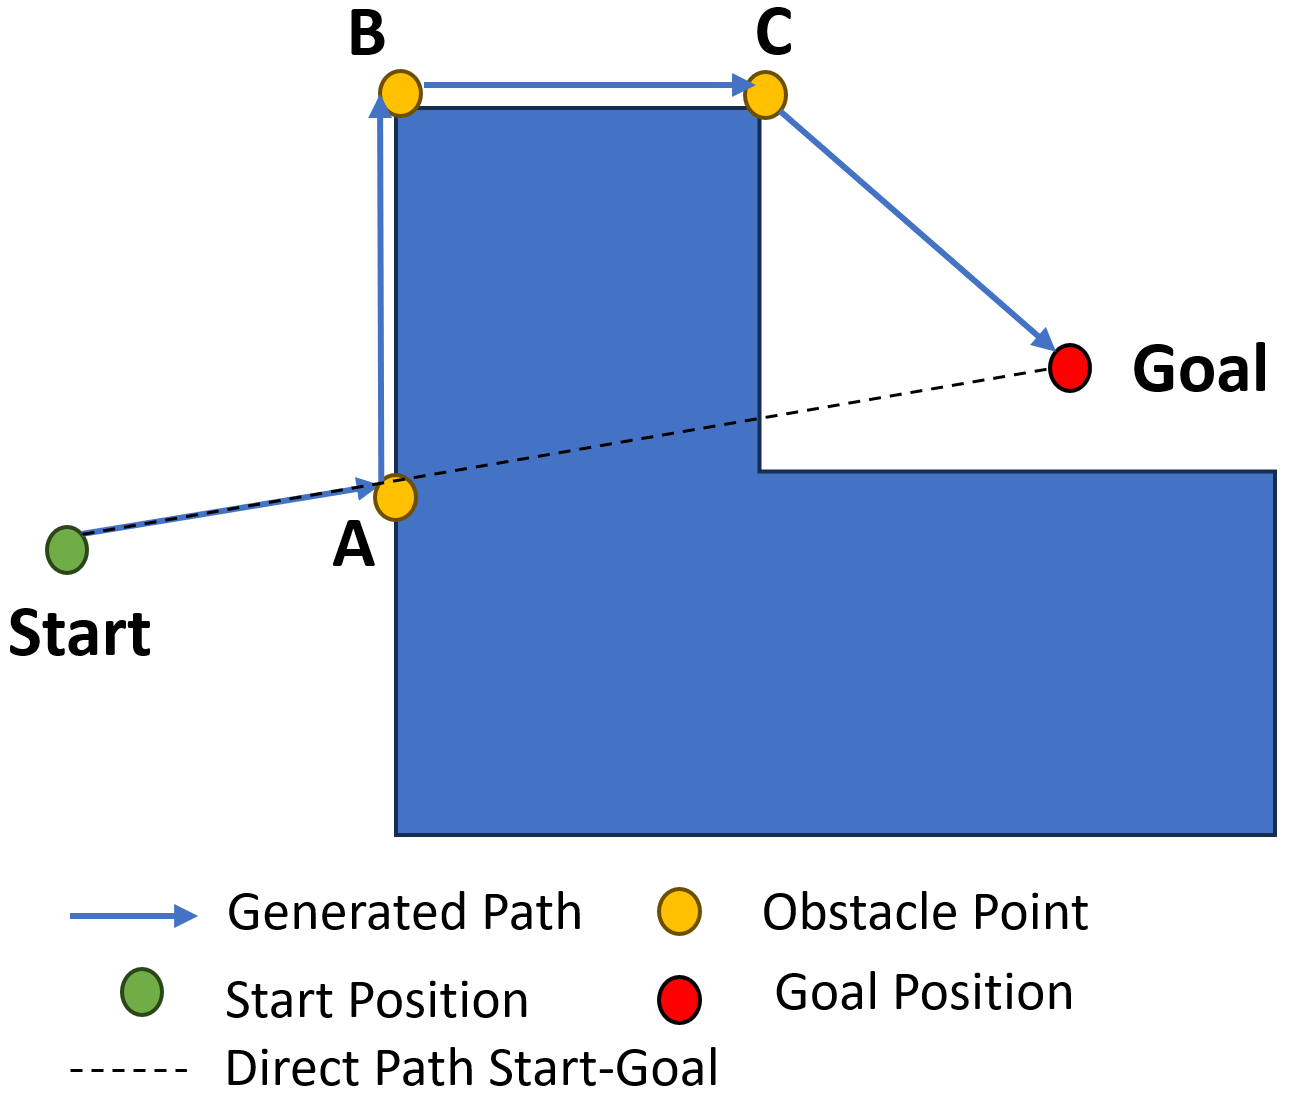
\includegraphics[width=3in]{images/Chap1/Bug_Algo.png}\\
        \caption{Bug Algorithm Path Solution to navigate from Start to Goal while avoiding
        the obstacle}
        \label{Bug_Algo}
        \end{center}
\end{figure}

\textbf{Velocity-generating path planning methods} are algorithms used in AMRs, to calculate both 
the speed and direction of movement. They predict the rotational and translational velocities 
creating the state space of velocities and taking into account the sensory inputs \cite{R28}. 
The Dynamic Window Approach (DWA) is a Velocity-generating path planning method.

In \cite{R19}, Liu et al. used Djikstra ALgorithm (A path-generating Algorithm) 
for Global path planning and 
the DWA as the local path planner for sudden unknown obstacles that could 
appear for smart cars while following the global path.
It works by evaluating different possible movements the robot could make within a short time frame 
and choosing the one that avoids obstacles while also moving towards the goal. The "window" refers 
to a limited set of possible velocities of the velocity space the robot can use based on its current 
speed and capabilities. Figure \Ref{flowchart of the DWA} details the flowchart of the DWA. 

The DWA algorithm starts by analyzing the car's position and base data. It then samples the speed and 
generates a range of possible trajectories. Each trajectory is evaluated to check if it will collide with 
obstacles. If a trajectory is collision-free, it's considered for optimal trajectory selection. This process 
continues until all possible trajectories have been evaluated, or an optimal one is found.
The combined algorithms were tested on 3 spaces with 3 stages of environment complexity ranging from 
simple to complex. However, the tests were effected with dynamic obstacles only inside the simulation and
so it is subject for the reality gap problem.
While these methods excel at avoiding obstacles at high speeds, they struggle with local minima. This is 
because they don't consider the overall structure of the free space when evaluating movements.
Additionally, these velocity-generating methods have limitations in mapping the future movements of 
non-holonomic platforms. For example, a method might suggest a movement that is impossible for the 
vehicle to perform due to its non-holonomic nature \cite{R28}.

\begin{figure}[H] 
\centering  
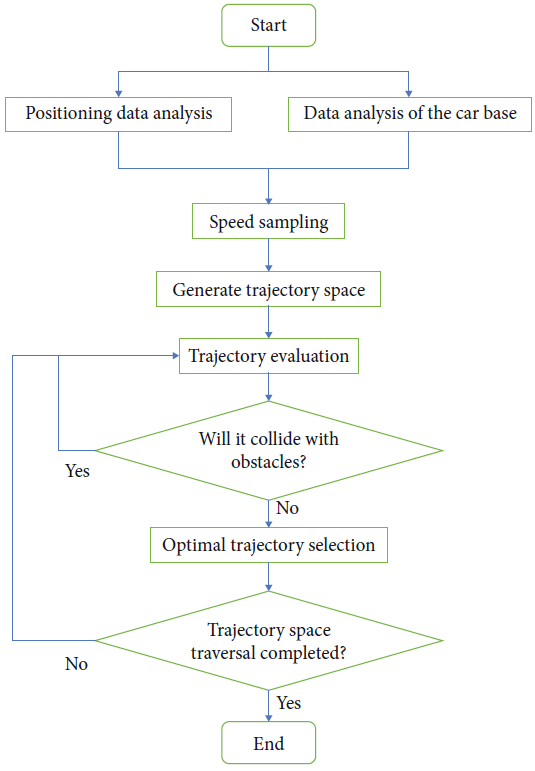
\includegraphics[width=3.5in]{images/Chap1/DWA_flowchart.png}  
\captionof{figure}{Flowchart of the DWA \cite{R19}}  
\label{flowchart of the DWA}  
\end{figure}

\textbf{Path-generating path planning methods} plan entire trajectories in advance, considering both the 
vehicle's position and its intended path over time. These planned trajectories are then combined with 
the previously calculated overall path. Currently, various path planning methods are used in both industry 
and research \cite{R28}.
For example, A* Algorithm is a Path-generating Grid-based method where
the environment is partitioned into a grid of discrete cells, where each cell represents a 
portion of the space. 
The algorithm then traverses these cells to identify suitable paths based on factors such as occupancy 
or cost. For example, in the A* algorithm, the fitness function is calculated from the start point 
to the reached cell, while in the Dijkstra algorithm, it's from the reached cell to the destination. 
While this approach offers a straightforward understanding and implementation, its computational cost 
can be significant due to the large number of cells to evaluate and the repetitive nature of the 
calculations. Additionally, grid-based methods are often constrained by the fixed directionality 
of the grid. The paths generated are restricted to the directions defined by the grid. 
For instance, if the grid is aligned along the x and y axes, the robot can only move horizontally 
or vertically. This can be inefficient or even impossible in environments where diagonal 
or more complex movements are required.
On the Other hand, 

Lavalle \cite{R47} created a method called Rapidly-exploring Random Trees (RRT), a randomized data structure used 
for various path planning tasks. It starts with a single node (usually the starting point)
and iteratively grows a tree by adding new nodes. At each iteration, a random point is sampled from 
the search space. The nearest node in the tree is found, and a new node is added along the path to 
this random point. This process is repeated until a path is found or a maximum number of iterations 
is reached. RRT is particularly effective for exploring complex environments with obstacles. 
Figure \Ref{sampling-based}, illustrates the test of RRT in an obstacle-rich environment (shown in blue)
using 1, 4, then 32-core processors. The planned paths (branches) are shown in grey. 
The path calculated as optimal is shown in red and connects the start pose with the goal pose.
These algorithms present advantages like handling big environments and complex obstacle
situations, however, they can also be computationally intensive and demanding in complicated situations.
Figure \Ref{sampling-based} shows the difference in the resulting optimal path in a cluttered environment where with
1 core the algorithm successfully finds a feasible path, and, as the cores double, the computed path
improves its quality as the search tree expands. 
RRTs require collision checks for each new node, which can be computationally expensive and memory-intensive, 
especially in environments with numerous obstacles, heavy traffic, or complex paths.


\begin{figure}[H]
    \begin{center}
       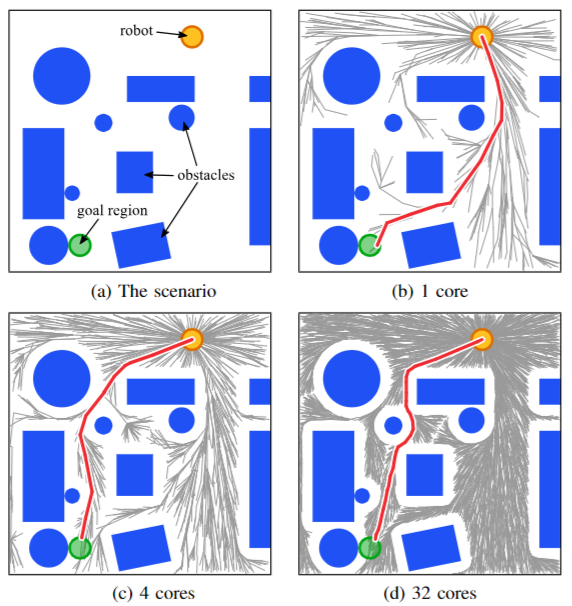
\includegraphics[width=3.5in]{images/Chap1/sampling-based.png}\\
       \caption{RRT ran on a non-holonomic robot using 1, 4, then 32-core 
       processors \cite{R16}}
       \label{sampling-based}
       \end{center}
\end{figure}

\textbf{Artificial Intelligence-based methods} 
leverage the use of Neural Networks, Fuzzy Logic, Reinforcement Learning, and Evolutionary algorithms. 
These methods learn from experience, adapt to changes, and optimize paths in complex environments. 


To start with, Neural Networks (NN) are inspired from the biological harmonious connection of the brain neurons
that gives it the ability to process big amounts of data and generate ideas and decisions and solve problems. 
The NN is built in a way that enables it to get its input in a form of data and process it by learning, improving 
and adjusting the output to the desired results. NN are able to perform Parallel processing: the information is 
transmitted in two
directions to the neuron in the case of Recurrent Neural Networks (RNN) that allows for learning from current and 
past inputs to the NN. This approach improves the computation time and overall performance. 
The NN is then able to process solutions that create paths for difficult environments. 
However, it presents a practicality challenge. Although the performance and results can be impressive, yet, in a 
real-time context, 
it is unfeasible to rely on solutions that require extensive computational efforts and need long durations to 
process solutions. In addition, the number of neurons and layers have to be scalable and depends closely on the 
level of complexity that the vehicle is to deal with: NN are trained using a use case so the 
outcome is tightly related to that use case and is not as efficient in other applications \cite{R12}. 

On the other hand, Reinforcement Learning (RL) can be used to learn optimal paths by interacting with the environment. 
The robot learns a policy that maximizes cumulative rewards, where rewards are given for reaching the goal, avoiding 
obstacles, and minimizing path length. The policy is often represented by a neural network, and the path is optimized 
as the robot learns from its experiences. Reinforcement learning (RL) methods for path planning in wheeled mobile robots 
face significant limitations due to high computational costs and long training times. These methods require extensive 
data to cover various scenarios, making the process time-consuming and resource-intensive. Training an RL agent, 
particularly in complex environments, can take millions of interactions, which is impractical for real-time applications. 
Additionally, as the environment's complexity increases, the state and action spaces expand, 
leading to scalability issues and longer training times. When combined with deep learning, RL becomes even more 
computationally demanding, requiring substantial resources and careful tuning of hyperparameters.

Fuzzy Logic (FL), on the other hand, is a way of thinking that mimics how humans make decisions, especially when things are unclear 
or uncertain. Instead of working with exact numbers, it uses "fuzzy" terms like "good", "average" or "bad" to make 
decisions. Input numbers are clustered following the fuzzy sets or intervals and assigned a value using membership 
functions. Later the values are interfered and defuzzified to generate the output as a command value. 
In robotics and path planning, FL helps robots navigate by allowing them to handle uncertain situations, 
like avoiding obstacles or finding the best route, even when the environment is not fully known. Instead of needing 
exact data, the robot can employ fuzzy terms like "close" or "far" to understand its surroundings. For example, if an 
obstacle is "somewhat close," the robot can smoothly adjust its path to avoid it. FL also helps the robot choose the best 
route by weighing factors like distance, even when the information is not fine-tuned. This improves the 
robot's handling of dynamic environments and making flexible and optimal decisions.
However, one 
disadvantage is that it can be tricky to create the right rules for the robot to follow, and the system can become 
complicated as more rules are added. It may present a scalability problem because in unpredictable and dynamic environments
it is not evident to overfit fixed fuzzy sets to be practical in all the cases \cite{R12}.

While Neural Networks and Fuzzy Logic offer powerful approaches for handling uncertainty and complex decision-making, 
another key area in artificial intelligence for path planning is the use of meta-heuristic algorithms.
Metaheuristic algorithms are inspired from biological and natural processes for evolution and survival. 
Relying on environmental input like obstacles and targets, meta-heuristic algorithms explore the solution
space by evolving random solutions for the problem and optimizing them by rounds until a stopping criterion or set
of criteria is satisfied (see more in section 4: Heuristic Approaches).
Approaches like Genetic Algorithms (GA) have been used for path planning by Ahmed Elshamli et al. \cite{R17}. The robustness of their 
solution is its adaption to dynamic environments. They evolve their GA using variable size chromosomes, where each node 
represents a waypoint of the path, then they measure the quality of each path using an evaluation function. A modified Genetic Approach is then 
applied to each population: Crossover, mutation, \textbf{Repair} infeasible paths, \textbf{Shorten}, then \textbf{Smoothen} 
feasible paths while dynamically checking for new obstacles.
The approach is tested in static and dynamic environments and has achieved proven efficiency when it comes 
to local optima challenges and surviving the best elements of the population. While the use of the GA itself is robust
and successful, it can be challenging to recreate the algorithm and to add the improvements. In addition, the tests
the ran are limited to a simple simulation with unrealistic situations and obstacle setting as displayed in 
figure \Ref{R17 test scenarios}: In reality, the hardware used to detect surrounding objects are scan based sensors
for instance LiDAR. They scan \(360^{\circ}\) of the surrounding starting from the robot as the origin.
This scan provides a polar perception of the obstacles (see figure \Ref{scamSim}). 
A polar perception only renders the perceivable surface of the objects.
The objects' depth and dimensions are not available through this sensorial input.
Obstacle perception is challenging due to limited knowledge of their exact contours and the 
discrete nature of optical sensor scanning. Connecting perceived points to form closed contours can 
be ambiguous, especially at a distance.

\begin{figure}[h!]
    \centering
    \begin{minipage}{0.30\textwidth}
        \centering
        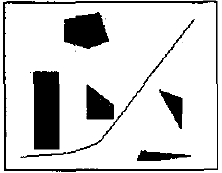
\includegraphics[width=\linewidth]{images/Chap1/R17_simple.png} % Replace with your figure
        \caption{Simple obstacle environment       }
        \label{Simple obstacle environment}
    \end{minipage}
    \begin{minipage}{0.30\textwidth}
        \centering
        
\includegraphics[width=\linewidth]{images/Chap1/R17_intermediate.png} % Replace with your figure
        \caption{Intermediate obstacle environment}
        \label{Intermediate obstacle environment}
    \end{minipage}
    \begin{minipage}{0.30\textwidth}
        \centering
        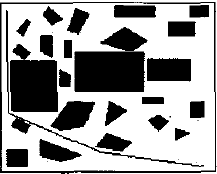
\includegraphics[width=\linewidth]{images/Chap1/R17_complex.png} % Replace with your figure
        \caption{Complex obstacle environment}
        \label{Complex obstacle environment}
    \end{minipage}
    \caption{GA Test scenarios \cite{R17}}
    \label{R17 test scenarios}
\end{figure}

While Classic path planning methods (Path-generating, Velocity-generating, and Direction-Generating) 
have proven effective across various applications and use cases, 
they often face challenges when applied to highly structured, repetitive environments like those found 
in industrial automation. To overcome these limitations, the research in the previous years became rather 
oriented to investigating and using heuristic approaches. In \cite{R26}, Masehian et al. conducted a 
chronological review about the followed approaches in Motion Planning (MP). The results testify that in 30 years,
The application of Heuristic approaches in MP went from 0\% to 54\% from 1977 to 2007 as shown on Figure 
\Ref{heuristic barchart}.

\begin{figure}[H]
    \centering  
    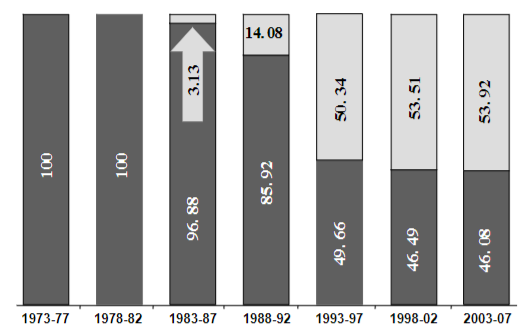
\includegraphics[width=3.5in]{images/Chap1/heuristic_barchart.png}\\ 
    \captionof{figure}{Application of classic and heuristic approaches in MP \cite{R26} 
    \newline \textbf{Dark gray:} Classic approaches
    \newline \textbf{Light gray:} Heuristic approaches }
    \label{heuristic barchart} 
\end{figure}

To draw to a close, even though the heuristic approach prevails the classic one:
\cite{R20} and \cite{R25}, these approaches are not without their limitations. Heuristic methods, while good at 
navigating complex environments and avoiding local minima, sometimes fall short in finding the best possible 
solutions, especially in high-dimensional spaces.

\subsection{Discussion: Selection of the Path Planning Method}

Path-generating methods are particularly promising for intralogistics applications involving autonomous 
mobile robots (AMRs). Unlike direction-generating methods, these methods are well-suited for dynamic environments. 
These methods effectively handle dynamic environments and disturbances while minimizing oscillations and 
computational costs.
They can also incorporate kinematic constraints and generate optimal trajectories in complex, unstructured areas. 
Compared to speed-generating methods, path-generating methods allow for dynamic planning horizons, enabling the 
calculation of optimal routes that avoid dynamic obstacles and disturbances. Given these advantages, this work 
will focus on path-generating methods for subsequent developments.


To enhance the efficiency and effectiveness of path planning, innovative approaches are emerging. 
By combining traditional methods with cutting-edge optimization techniques, we can overcome the 
computational challenges and achieve more robust solutions. These hybrid strategies offer a 
promising path forward, paving the way for advancements in path planning technology.



\section{Heuristic Approaches}
%intro
This section will focus on the Application of heuristic algorithms for solving robotic path planning 
problematics. 

\subsection{Optimization Techniques}
Optimization refers to the decision-making led by the machine with availability of certain circumstances and constraints
that either help or limit the outcomes of the optimizer \cite{R37}. In the case of path planning, optimization aims
to modify some properties of the generated solutions to cope with the surrounding conditions.
In stochastic environments, it is challenging to plan feasible paths given the high dynamics 
and obstacles.
The increase in the complexity of the environment and the constant dynamics increase the number of variables involved 
in the mathematical representation of the problem. As a consequence, it raises the computation efforts that need to be 
deployed for the creation and optimization of the solution and decreases feasibility \cite{R7}.
In order to get optimal results like smooth and short paths, finding a feasible path is not enough. The evaluation 
of the generated path and the optimization are helpful to ensure that the robot is driving the optimal path.
There exists a range of planners and optimizers which are clustered as classic and Heuristic approaches \cite{R12}.
Classic approaches include \textbf{Analytical} and \textbf{Enumerative} methods. 
The former rely on mathematical modeling, which can become unsolvable as the navigation environment becomes more 
cluttered. Additionally, applying these models can be challenging in scenarios where the necessary models for different 
components are not readily available. The latter have the drawback of increased intricacy in bigger or more elaborate 
search spaces. On the other hand, Heuristic approaches can be sub-categorized into \textbf{Meta-Heuristic} and \textbf{Evolutionary algorithms}.
Some of these methods can fall in the trap of local minima and sub-optimality \cite{R12}
Alternatively, after a review of the available planning and control approaches in intralogistics, Fragapane, G. et al. \cite{R7}, 
concluded that nature-inspired algorithms can instill intelligence into planned paths.
Elshamli, A. et al. explained in \cite{R17}, that Meta-Heuristics are adaptive to the dynamics of the surroundings
unlike classic approaches that proceed sequentially to generate solutions. The paths developed by classic approaches
can thus become infeasible in a later stage if the environment changes. Metaheuristic approaches are based 
on parallel search mechanisms that can have updated input of the conditions and thus are more adaptive and 
practical in real-world scenarios.

Next, this section dive into Meta-Heuristics which are defined by Bilal et al. as 'the optimization
techniques mainly based on function evaluation and make little
or no use of the properties of objective functions and constraints.
Meta-heuristics are thus problem independent techniques not taking
advantage of any specificity of the problem’ in their review \cite{R37}.
The authors later break down Meta-Heuristics into \textbf{Neighborhood-based Algorithms} and \textbf{Population-based Algorithms}
as given by the tree graph in Figure \ref{Tree}

\begin{figure}[H]
    \begin{center}
        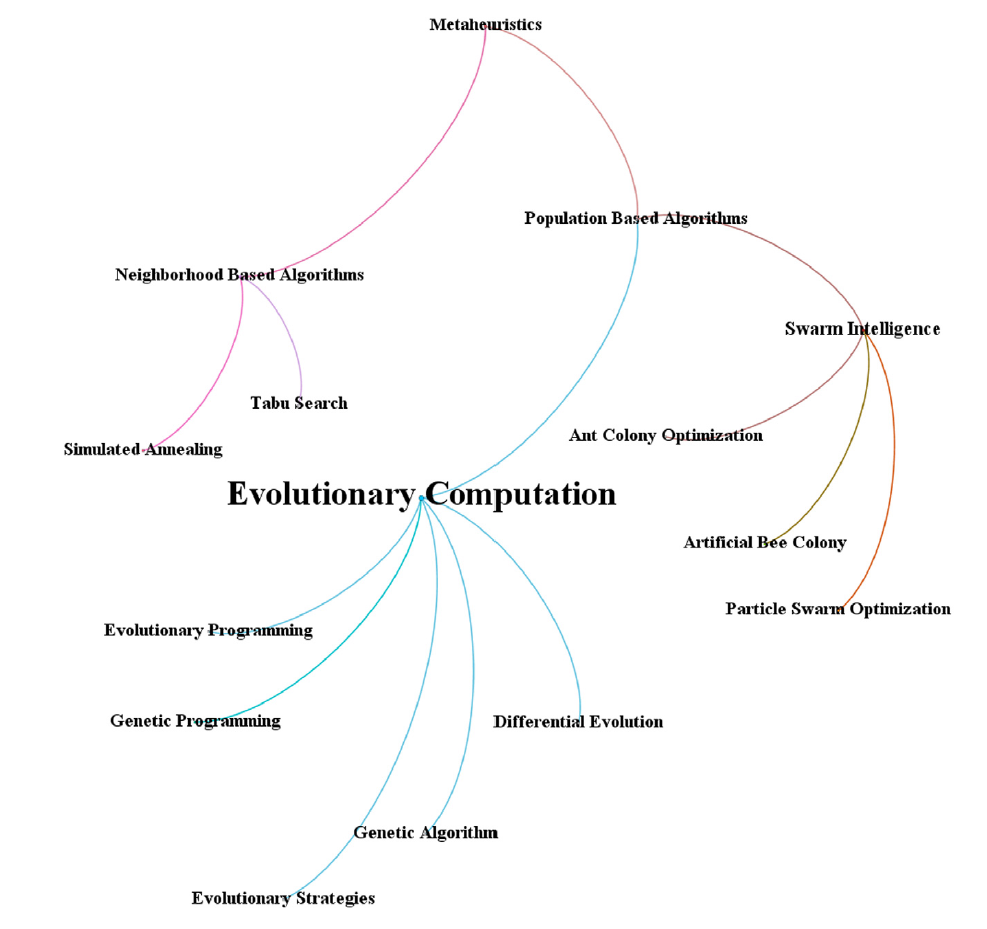
\includegraphics[width=\linewidth]{images/Chap1/Tree_Metaheuristic.png}\\
        \caption{Tree of Meta-Heuristic Algorithms \cite{R37}}
        \label{Tree}
    \end{center}
\end{figure}

The Neighborhood-based algorithms benefit from the neighboring solutions by migrating from the current solution to 
the near surrounding solutions with the goal of improving the fitness function. The examples mentioned for this 
approach are Simulated Annealing (1979) and Tabu Search (1989). The Population-based algorithms are methods that start from a sample population and rely on their evolutions. 
They are inspired by the evolutionary processes observed in nature and are sub-categorized in this approach under 
Swarm intelligence and Evolutionary Algorithms. 
Swarm Intelligence approaches are analogous to the socio-cooperative practices of species like bees, ants, and birds. 
For instance, Ant Colony Optimization (1992)and Particle Swarm Optimization (1995) are examples of such algorithms. 
On the other hand, Evolutionary algorithms rather copy the species evolution theory, among which are Differential 
Evolution (1995) and Genetic Algorithm (1957) \cite{R37}.

Metaheuristics, mainly Swarm-based methods and Genetic Algorithms, 
have been used multiple times for robotic path planning, as noted in the literature. 
Each algorithm has its own unique search methods and strengths, providing different benefits and 
areas for optimization.
  


\begin{figure}[H]
    \centering
    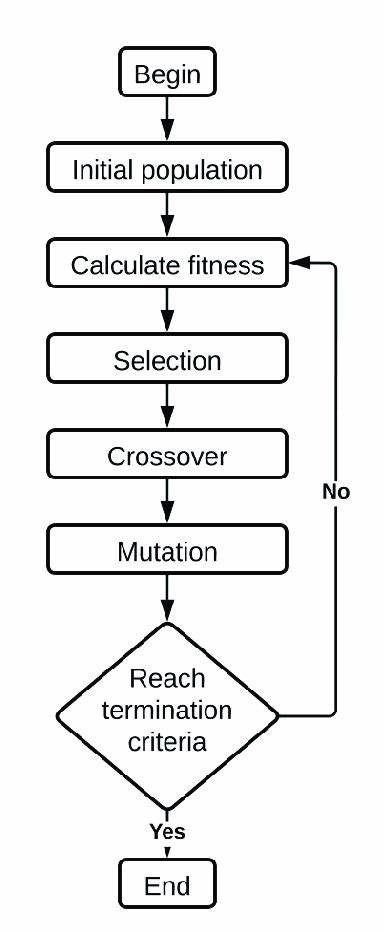
\includegraphics[width=2in]{images/Chap1/GA.jpg}
    \caption{Flowchart of the GA \cite{R39}}
    \label{GA}
\end{figure}

Elshamli, A. et al. \cite{R17} have employed the Genetic Algorithm (GA) (See algorithm steps in figure \Ref{GA}) to solve 
the problem of path planning in dynamic environments. They represent their paths using chromosomes where each node of the chromosome represents 
a waypoint and develop a variable chromosome length approach that accommodates obstacle avoidance and efficiency 
in reaching the goal. The fitness of each chromosome is evaluated according to an objective function that includes path length, smoothness, 
and clearance to obstacles. A modified genetic Algorithm is applied where after crossover and mutation, paths are 
shortened and smoothed if it is possible. Saving the best individuals generated by the GA was effective in delivering the overall best solutions.
Tamilselvi, D. et al. also modified the GA by applying the elitism concept. 

This is achieved by saving the best individual, denoted as \(S_{best}\), and replacing the worst individual in the 
next generation with \(S_{best}\). This approach helps to prevent premature convergence to local optima, increasing 
the likelihood of finding the global optimum. In the context of path planning, elitism has proven effective 
in discovering feasible paths in environments with limited dynamic obstacles. Additionally, by incorporating 
a motion prediction mechanism based on the grid map, elitism can be adapted to handle dynamic obstacles more 
effectively \cite{R38}.

Authors of \cite{R40} also worked on the path planning in dynamic environments' problem. They critic the GA to be computationally
intensive and to require long planning time. Instead, they suggest the Simulated Annealing algorithm (SA)
to solve the path finding problem. 

\begin{figure}[H]
    \centering
    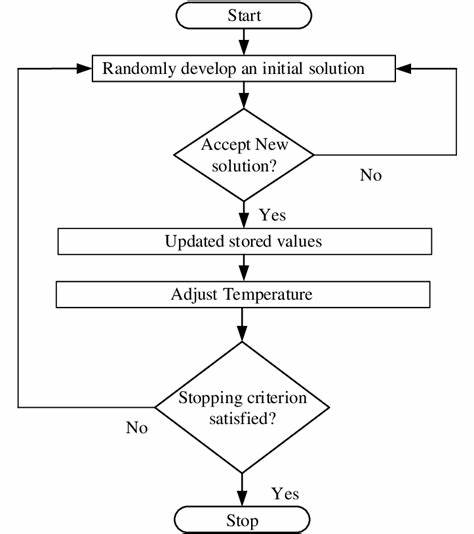
\includegraphics[width=3.5in]{images/Chap1/SA.jpg}
    \caption{Flowchart of the SA \cite{R41}}
    \label{SA}
\end{figure}

Being a probabilistic meta-heuristic algorithm it is designed to guide the local
optimum to a global optimum. The approach is based on the evaluation of the path length to discriminate 
path candidates: the shorter the path the better. It works by trying out different paths for the robot, beginning 
with a high "temperature" that lets the algorithm accept good paths and bad paths with a accepted with a certain probability,
which decreases over time (simulating the cooling process in annealing). This helps it explore a wide range of 
options and avoid getting stuck in local minima. As the process continues, the temperature slowly decreases, 
making the algorithm less likely to accept bad paths, and helping it to focus on finding the global minima as given by 
figure \Ref{SA}. algorithm was tested in four environments with different static and moving obstacles. The algorithm 
successfully found the best or nearly the best paths and could quickly adjust to avoid collisions in real-time. 
Compared to a genetic algorithm, the SA method was 57\% faster for complex environments and 74\% faster for simple
environments. However, the processing time increases exponentially for complex environments (13.57 seconds).

Particle Swarm Optimization Algorithm (PSO), as well, is used for solving non-linear optimization problems like scheduling, power 
management and also robotic path planning. It is inspired from the cohesive behavior of bird and fish swarms traveling 
together.It works by having a group of particles (potential solutions) move around in the search space to find the best 
solution. Each particle in the PSO algorithm remembers the coordinates of the best solution it has found so far, known 
as its personal best \(pbest\). Additionally, the algorithm tracks the best solution found by any particle, referred to as 
the global best \(gbest\). The core idea of PSO is to guide each particle towards both its \(pbest\) and the \(gbest\) positions:
from state a to c as given by figure \Ref{pso}, 
using a randomly weighted acceleration during each iteration. The algorithm iteratively updates the particles' positions 
and velocities until an optimal or near-optimal solution is found.
Alaliyat, S. et al. have investigated dynamic environment navigation using PSO. They found out that the performance 
of the algorithm depends on parameters tuning. Overall, feasible paths were successfully generated.
Planning time is rather high for simply organized environments (18.35s) and higher for the most complicated scenario
(31.17s).

\begin{figure}[H]
    \begin{center}
        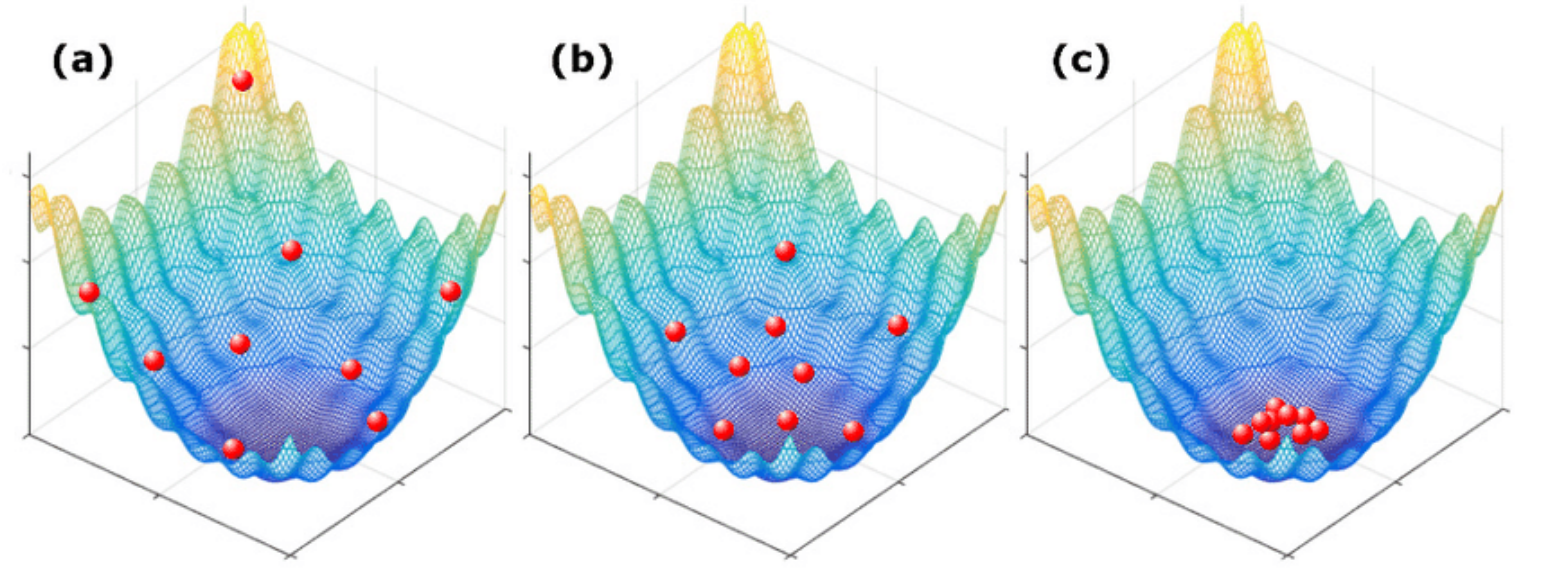
\includegraphics[width=4in]{images/Chap1/PSO.png}\\
        \caption{Particle Swarm Optimization \cite{R42}}
        \label{pso}
    \end{center}
\end{figure}

Differential Evolution (DE) has been used in a hybrid algorithm along with PSO by Tand, B. et al. \cite{R43} to leverage 
both of the algorithms benefits. DE is rarely solely applied to path planning problems. In their review \cite{R37}, 
of 20 years of research about DE, Bilal et al. did not mention robotics among the fields of application of DE. 
DE starts with a set of potential solutions. Each solution, or individual, is modified 
through mutation, crossover, and selection to improve over time. Mutation introduces random changes to create new 
candidates and avoid getting stuck in local optima. Crossover mixes parts of the new candidates with the original 
solutions to explore new possibilities. The selection process keeps only the better solutions for the next generation. 
This method effectively balances exploring new options and refining existing ones, making DE well-suited for complex 
optimization tasks.
By integrating improved PSO and DE algorithms for enhancing particle diversity, Tand, B. et al. achieved better 
path quality compared to other methods. The results demonstrate that their approach outperforms traditional 
evolutionary algorithms in path optimality and optimize computation times by 1.38\% \cite{R43}. 

Ant Colony Optimization (ACO) is known for being robust and good at parallel processing, but it can be slow and 
sometimes gets stuck in local optima solutions. To fix this, improvements like Ant Colony System (ACS) 
and Max-Min Ant System (MMAS) have been developed, which make ACO better at finding solutions but still have 
issues like being too rigid and converging too early. In mobile robot path planning, new strategies have been 
created to address these problems, such as adaptive methods that improve how pheromones are updated and balance 
exploration with finding the best path. Recent research has also introduced advanced versions like polymorphic 
ACO and multi-objective optimization, making ACO more effective for real-time and complex situations. However, 
these improvements also make the algorithm more complex and take more time to compute.

%advantages & limitations in discussion:

Meta-heuristic algorithms, such as Genetic Algorithms (GA), Particle Swarm Optimization (PSO), and Differential 
Evolution (DE), have become increasingly popular in robotic path planning. These algorithms are attractive because 
they can find good solutions to complex problems by mimicking natural processes like evolution or swarming behavior.
However, despite their growing use in research and their potential efficiency in practical use cases, the application 
of meta-heuristic algorithms in real-world robotic path planning like the intralogistics field remains quite limited. 
One of the major issues is that most studies focus on simulations rather than 
testing in real environments. While simulations can help develop and adjust these algorithms, they do not fully 
cover the challenges robots face in the real world, such as varying conditions, surface types, or unexpected 
noises. Another major issue is how obstacles are represented in these studies. Often, obstacles are either unrealistically 
large compared to the robot or have overly simple shapes that don’t accurately reflect real-world conditions. This 
lack of realism can result in algorithms that work well in simulations but fail when used in real environments. Additionally, 
because these algorithms are mostly tested in controlled, simulated settings, they may be too finely 
tuned to those specific conditions. This can make them less reliable when applied to the unpredictable conditions 
of the real world gap. In summary, while meta-heuristic algorithms show promise for robotic path planning, more real-world 
testing and realistic obstacle modeling are needed to ensure they work effectively in practical situations. 
Addressing these issues is key to advancing the use of robotics in intralogistics and other fields.
\newpage
\section{Discussion} %TODO: change name it is soa here
To synthesize the research conducted, it is paramount to summarize the \textbf{key concepts} comprehensively and 
point out the general \textbf{drawbacks}. This 
State-of-the-Art report focuses on mobile robot path planning, a critical component of the overall 
robotic planning process. Effective path planning not only organizes and optimizes a robot's navigation 
but also significantly enhances its productivity by enabling it to execute missions more efficiently. 
In dynamic environments, a well-designed path planner is essential for ensuring safe operations and 
maximizing the robot's resource utilization and operational capacities.
Meta-heuristic optimization algorithms are highly effective for refining mobile robot paths, particularly 
when building routes from scratch while considering both static and dynamic obstacles.
They also have the capability to solve problems without information about their mathematical model.
This has the great advantage of reducing the burden of expliciting the situation in order to solve it especially 
in complex cases where the effort to model the problem and the constraints is higher and, later, the computation 
is harder. Instead, meta-heuristic algorithms focus on optimizing the fitness function related to the specific 
use case. 

The path planning methods discussed have several drawbacks. Grid-based methods can be easily misled by noisy 
sensor data, and their generated paths might not be the shortest possible, particularly in crowded areas. 
Some methods excel at high speeds but struggle with dynamic environments, while others may have limitations 
in planning for non-holonomic vehicles. Computational efficiency is a concern, as some methods are slow and 
resource-intensive, especially in complex environments. Heuristic methods, while effective, might not always 
find the optimal solution. Real-world applications pose additional challenges. In dynamic warehouse settings, 
blocking areas for extended path planning can disrupt operations, interfere with other vehicles, and reduce 
productivity. Metaheuristic optimization approaches have been limited to mission scheduling in intralogistics 
robotics, with fewer applications in path planning. Addressing these limitations requires innovative solutions 
that balance computational efficiency, real-time performance, and path quality.

Furthermore, the classical and the heuristic approaches are capable of creating new different paths every time the 
algorithms are run even in the same environment setting. While this phenomenon proves of the intelligence of the algorithms
and the availability of several optimal paths, it makes the fully automated robot's behavior non-repeatable and unexplainable. 
For humans, it is difficult to foresee the behavior if many options are available. However, it is important for those working 
closely to robots to have an expectation of their behavior. It enables them to avoid collision risks and injuries and to 
plan their actions accordingly. If a predictable vehicle behavior is available, it promises a structured approach to path 
generation, reducing computational complexity and improving path quality.

Combining an optimal path planning approach that accommodates the kinematic constraints of Autonomous forklifts in the
intralogistics environment and generates smooth paths, is behaviorally explainable and deploys meta-heuristic 
Algorithms is a new approach that would have an added value to mobile robot path planning in intralogistics of 
reducing computation time and travel distance and improving AI driven solutions explainability. 

\section{Adopted Path Planning and Optimization Methods}

The above discussed Path Planning approaches are typically
designed to solve path planning problems in various environments and have been used in multiple
applications.
For this project's problem, the robot operates in a consistent environment—the station. 
Although stations may differ in 
position, size, and layout, the components within them remain the same: shelves containing pallets. 
This consistency suggests that we should 
develop a solution specifically tailored to the station environment, which would help minimize potential problems 
and reduce the effort required to solve them. 

A path planning module has already been developed at STILL for the autonomous 
forklift trucks, utilizing classic sampling-based path planning methods. This module is based on the Open Motion 
Planning Library (OMPL), an open-source library for motion planning in robotics. OMPL is designed for complex use 
cases and includes several algorithms, such as probabilistic roadmaps (PRM) and rapidly-exploring random trees 
(RRT), along with their variants. OMPL performs well in clean environments without obstacles, with a minimum 
processing time of \(200ms\), but in complex environments, processing time can increase to \(2s\).
While it can be very fast in the absence of obstacles this approach presents some limitations:
\begin{itemize}
    \item Not Station-Specific: While OMPL is a versatile and powerful motion planning library, its general-purpose 
    nature can be a limitation for station-specific pickup/drop operations. OMPL is designed to handle a wide range 
    of environments and tasks, but it may not be as efficient or tailored to the specific constraints and 
    requirements of station-related operations. OMPL may not have built-in knowledge or optimizations for tasks 
    like docking at specific stations, handling different station configurations, or considering constraints 
    related to station-specific equipment.

    \item Too Complex for Simple Tasks: OMPL's advanced algorithms, while powerful, can be overkill for simple tasks 
    like pallet handling. Its general-purpose nature can also lead to computational overhead, 
    especially in less complex environments. This suggests that tailoring OMPL to specific station-related 
    operations could improve its efficiency and effectiveness.
    
    \item Long Processing Time: OMPL's processing times can be substantial, particularly in complex environments 
    with numerous obstacles, tight spaces, or frequent changes in the environment. 
    This can lead to delays in decision-making and potentially hinder the overall efficiency of operations. 
\end{itemize}

Given OMPL's limitations, I propose a station-based approach is needed. This approach will be tailored 
to the structured environment of the station, enabling faster and more efficient path planning. 
By minimizing directional changes and adhering to station boundaries, we can achieve shorter and repeatable 
path calculation times, optimizing the overall efficiency of operations. By focusing on the typical tasks of pallet 
pickup and drop-off, we can create a solution that works effectively in simple and moderately complex 
situations, reducing processing time and resource usage. 

For optimizing paths, various approaches exist.
Path optimization can be approached mathematically using Jacobians, which map control inputs, like position or wheel 
speeds, to the desired outcomes. The objective is to minimize a cost function—such as path length, energy use, 
or time—by adjusting the robot's control inputs to achieve the desired position. A common technique is gradient descent, 
where control inputs are iteratively updated to reduce the cost. The Jacobian matrix, which links these 
inputs to the robot's position, guides these adjustments until the most efficient path is found. However, the Jacobian-based 
optimization method poses several challenges for this use case. For wheeled mobile robots with multiple control inputs, 
the Jacobian matrix can become complex and large, leading to increased computational costs and making real-time 
optimization challenging. 

Frequent updates in dynamic environments further add to this load, potentially leading to delays or suboptimal paths. 
Mukherjee et al. \cite{R44} noted that their approach to optimal trajectory planning does not guarantee a global 
optimum but rather an isolated local optimum close to the global one. Additionally, this method relies on precise 
kinematic and dynamic models, so any inaccuracies, such as sensor errors, can result in poor path optimization. 
In this context, the kinematic model would need to be refined for the specific truck using it. Managing complex inequality 
constraints, like obstacle avoidance, can also complicate the optimization process and reduce efficiency.

Reinforcement Learning (RL) offers a promising approach to learning optimal paths for mobile robots. By interacting 
with the environment and maximizing rewards, RL agents can develop effective policies. However, RL methods for 
path planning in wheeled mobile robots face significant challenges, including high computational costs, long 
training times, and the need for extensive data. These limitations make RL impractical for real-time applications 
in complex environments.

As highlighted in the previous Section , meta-heuristic approaches, though powerful for solving complex problems, 
often require significant computational time. However, this can be greatly reduced by optimizing how these 
methods are applied. Instead of generating a path entirely from scratch, this work proposes starting with a pre-built 
or partially constructed path provides a solid foundation. Additionally, reducing the number of waypoints 
can streamline computation, allowing the algorithm to focus on refining an already good solution rather 
than calculating every detail from the ground up. This approach preserves the strengths of meta-heuristics 
while significantly speeding up the planning process, making it more practical for real-time or near-real-time 
applications.

\section*{Conclusion}

In this chapter a detailed State of the Art related to Intralogistics, AMRs, Near-Field Planning, and Heuristic 
Optimization was laid out. The investigation of the literature helped to address the advantages and limitations
of individual approaches and decide around the relevant approaches to the Problem Statement. 
A Choice of the methodology was conducted at the end taking into account the compiled information.
In the following chapter, we will delve into the design and development of the solution 
combining a Path generating to Metaheuristic Optimization to obtain an optimal path.


\part*{Chapter 3 \\Design and development of the Control Interface}
\chapter{Design and development of the Control Interface}

\renewcommand{\chaptername}{Chapter}
\section*{Introduction}
In this chapter, we delve into the heart of the iHEX system's functionality – the Control Interface (CI) software which forms the cornerstone of communication and control, enabling seamless interaction between the MC and the SCs. This chapter presents the design, development, and test of the CI on both the MC and SC and the integration of both of them.

\section{Control Interface (CI) on the MC}
\subsection{Multithreaded architecture:}
In the design of the CI on the MC, a multithreaded architecture was adopted to meet the dynamic and concurrent demands of communication, command processing, monitoring, and logging within the iHEX system. The use of multithreading was essential in ensuring a responsive and efficient operation of the control software.

\subsubsection{Multithreading need}

A fundamental requirement for the Control Interface is its ability to handle multiple tasks simultaneously. The MC must efficiently \textbf{manage communication with the server}, \textbf{manage communication with the SCs via CAN Bus}, \textbf{continuously monitor the health of the CAN network}, and \textbf{maintain a log of system activities}. This multifaceted demand necessitates a multithreaded approach to prevent bottlenecks and ensure timely execution.

\subsubsection{The <pthread.h> library}


\part*{Chapter 4 \\Design and development of Printed Circuit Boards}
\chapter{Test and Validation of the Proposed Solution}

\renewcommand{\chaptername}{Chapter}

\section*{Introduction}
%After the development conducted in the previous chapter, the results of the implementation 
%and concrete tests are highlighted and discussed.
%This part outlines:
%
%* the initial conditions of the test: Coordiantes of the robot, and the coordinates of the station 
%and its configuration and constraints. and the test scenarios.
%* the results of path planning of the pattern path. 
%* results of the evaluation approach 
%* results of the path optimization
%* Analysis of the Metaheuristics
%* Comparison to OMPL
%* the robot following the generated path. Screenshots of the robot at 3 intermediate positions and mention 
%the coordinates. the robot in its final position.

This chapter presents the results of testing and validating our proposed path planning and optimization algorithms. 
We conducted experiments under various conditions, evaluating factors such as path quality, algorithm 
performance, and robot execution. By comparing our approach to OMPL and analyzing the results, we aim 
to demonstrate the effectiveness of our solution for real-world AMR applications.
For this section 3 test environments are used:
\begin{itemize}
    \item Independent Simulation Environment: This environment is created outside the RACK 
    environment to validate the chosen approaches before implementing the developed features 
    on the real system. It recreates the Station and the Shelf without sensor inputs or kinematic constraints.
    To simplify the test, the robot is modeled by a point instead of its proportional chassis size.

    \item RACK simulation environment: It is the simulation environment used in the team to simulate 
    the outcomes of the developed features in the same conditions as the real test. It includes all the sensor 
    input and makes it available for the test: Localization, Obstacle Detection, and Object Recognition features.
    It can be Offline or Online
    \begin{itemize}
        \item Offline Testing: is the re-creation of the warehouse and the test environment in a complete model
        as seen on figure \Ref{warehouse}. A simulated robot is available to place at a starting point, 
        to navigate the planned paths as well
        as to perceive its surroundings and use the sensor input for its processing. Objects like simulated 
        obstacles can be added. 
        \item Online Testing: is a projection of the test on the AMR to the Simulation environment.
        The simulation visualizes the output of the sensors like scan points and makes a debugging 
        tool available for interpretation of results, debugging, and optimization.
    \end{itemize}

    \item AMR Field Tests: the AMR is commissioned with the test algorithms, validated through the RACK simulation
    environment tests. The truck navigates the planned paths in the real warehouse and deals with real stations, 
    shelves, pallets, obstacles and general surrounding objects.
\end{itemize}

\section{Path Creation Test Results and Validation}
The implemented Path Creation Approach explained in section 3.2.3 was first tested in a simulation environment
composed of one Station. This environment emulates the RACK model of the test warehouse and was used to test 
and validate the approach before testing it inside the RACK simulation first and then on the AMR.

For this environment, the implementation results of the subpolygons from section 3.1 were used for the path creation.
The created subpolygons are used as transition zones. 
As a first test of pure path creation, the transition points are previously fixed at the center of the 
subpolygons. The path is created by placing the robot in the simulation in a starting position and testing 
different target locations.

The obtained results are of smooth splines adhering to the pattern and linking the truck to the destination pallet 
while passing by a transition location. 
The independent Simulation Environment tests show the pattern spline-based path as given by figure \Ref{Test_clone}:
The path start at the truck's position, transitions in one of the transition subpolygons to change driving 
direction and joins the target. 
The resulting path on the RACK simulation environment which is the real testing environment show as well 
the creation and plotting of the pattern path on the simulated station as given by \Ref{TestResults} and \Ref{Test_Simu}.

This approach is validated and is ready as a basis for the next test steps. 
The validation is for the following reasons:
\begin{itemize}
    \item The path creation module integrates the subpoygon functionality successfully: the use of a transition
    point from the subpolygons is effective when tested with a complete path.
    \item The created paths satisfy the intended pattern: they link the truck to the transition point, then, 
    the latter to the target. Inside the RACK simulation environment, it was verified that the direction 
    change occurs: the AMR switches from a negative speed at the first section when driving in opposite 
    direction the first part of the spline path until the transition point, to a positive speed when driving in 
    main driving direction the second part of the spline path from the transition point to the target.
    \item The paths link the start to the chosen target accurately which reflects the validation of the 
    transformations implemented at the development section of the Path Creation.
\end{itemize}

\begin{figure}[H]
    \centering
    \begin{minipage}{0.45\textwidth}
        \centering
        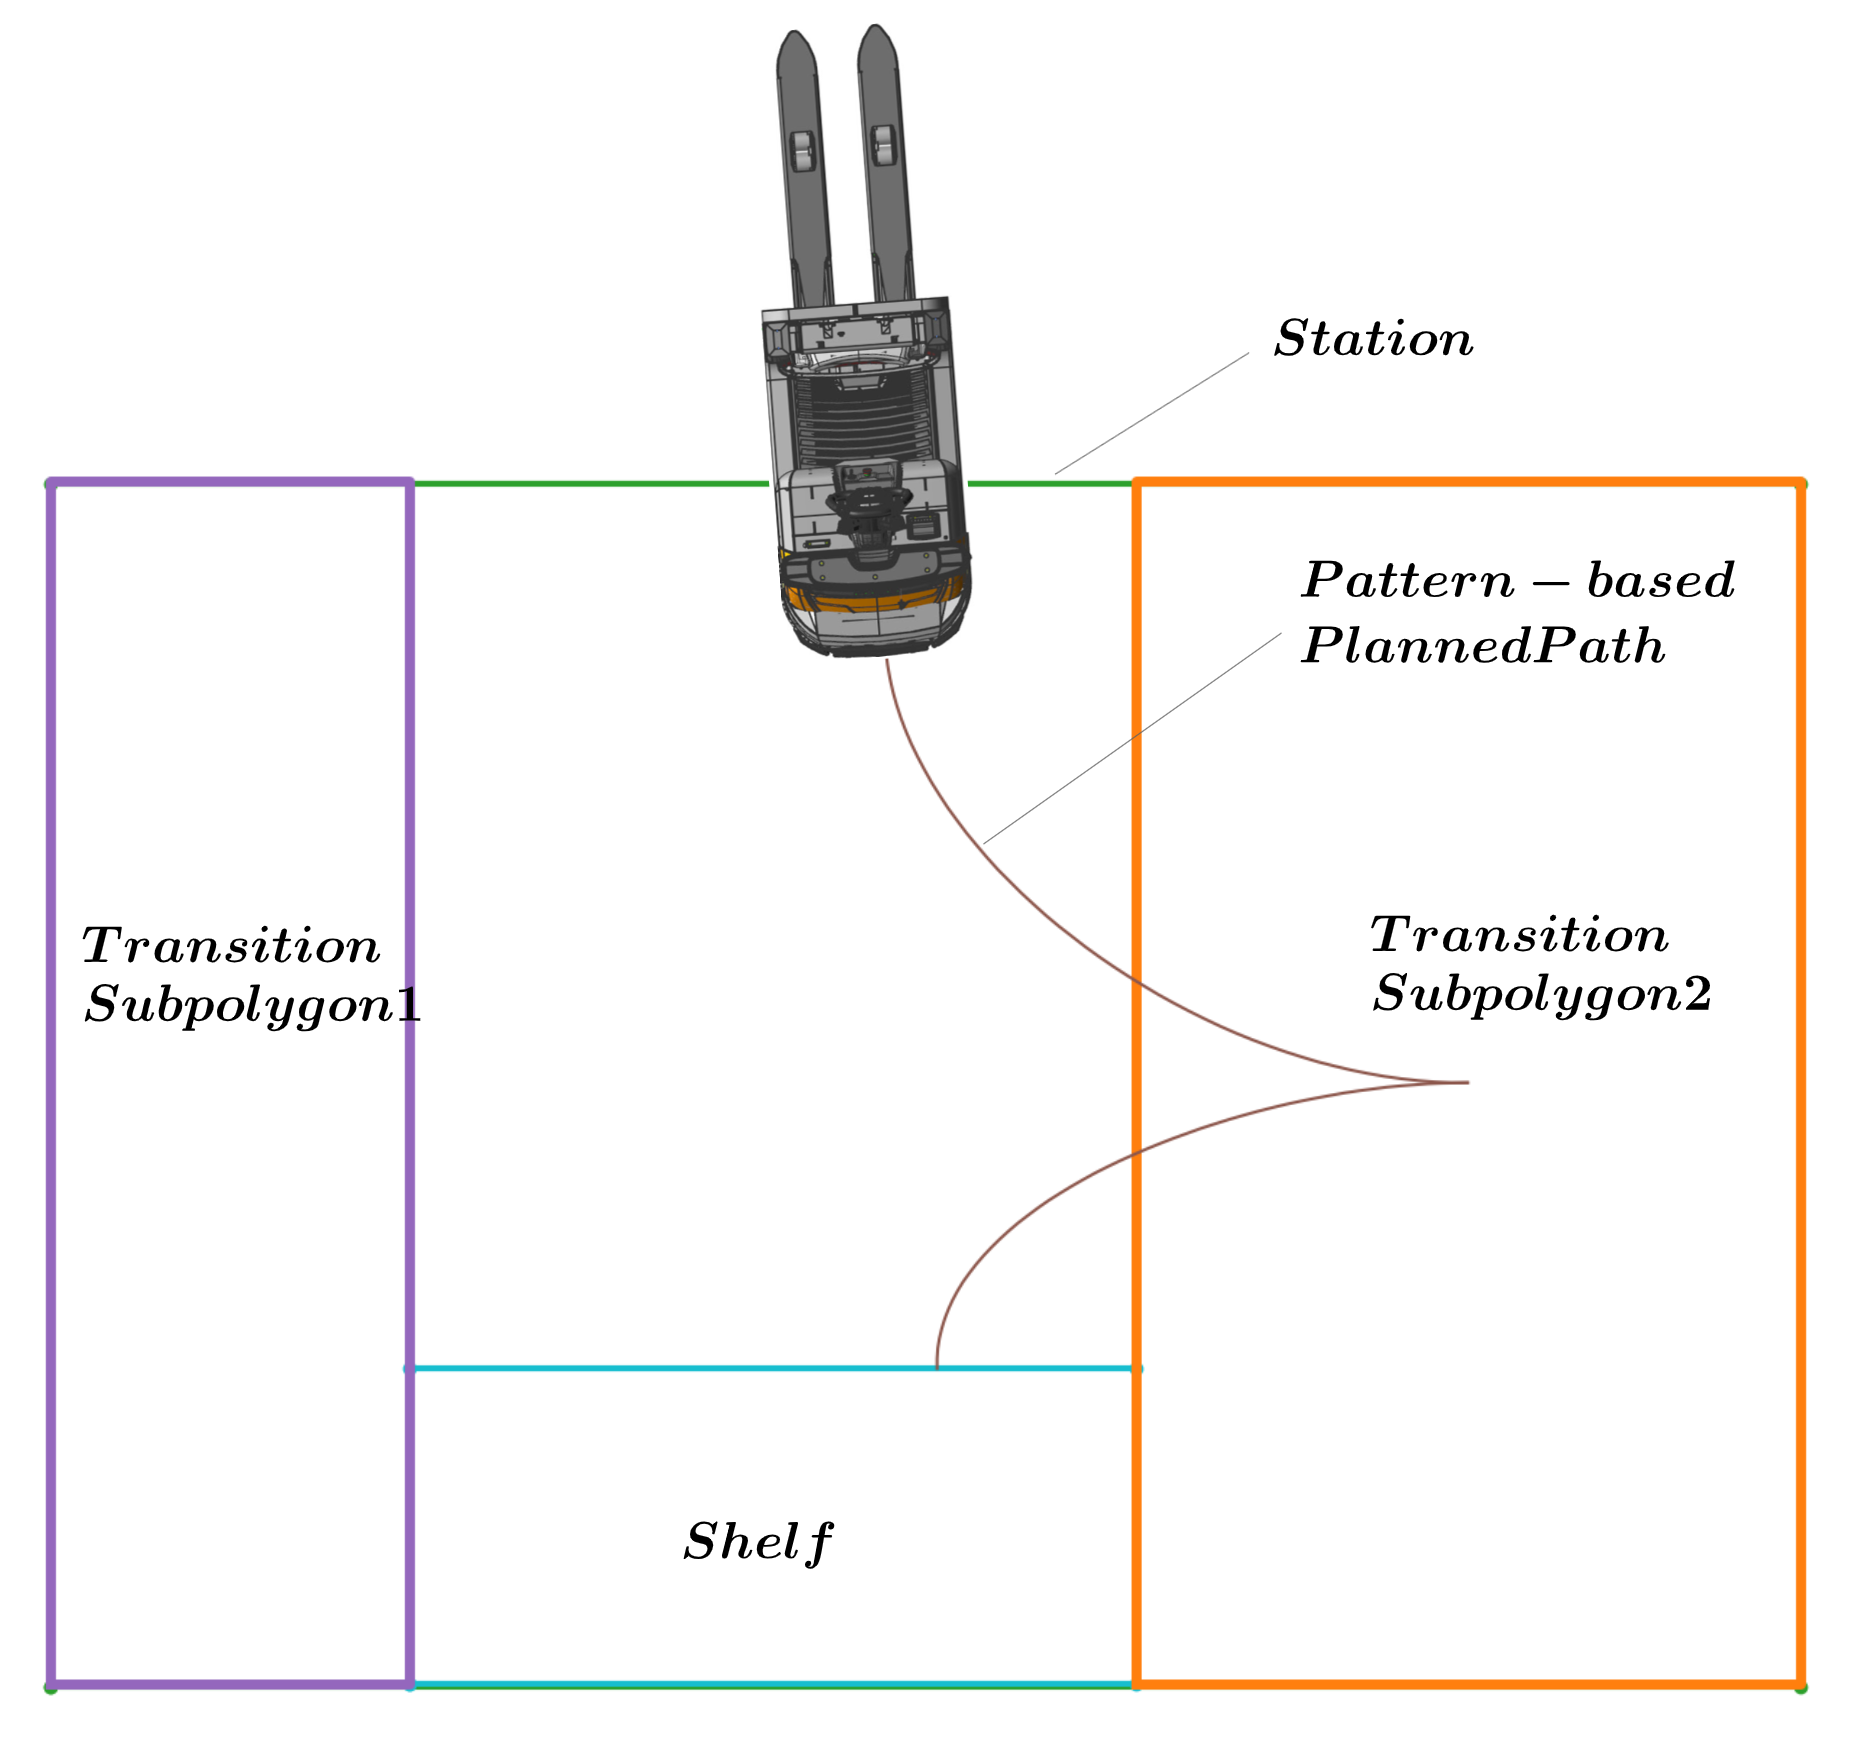
\includegraphics[width=3in]{images/Chap3/station1_pattern.png} 
    \end{minipage}
    \begin{minipage}{0.45\textwidth}
        \centering
        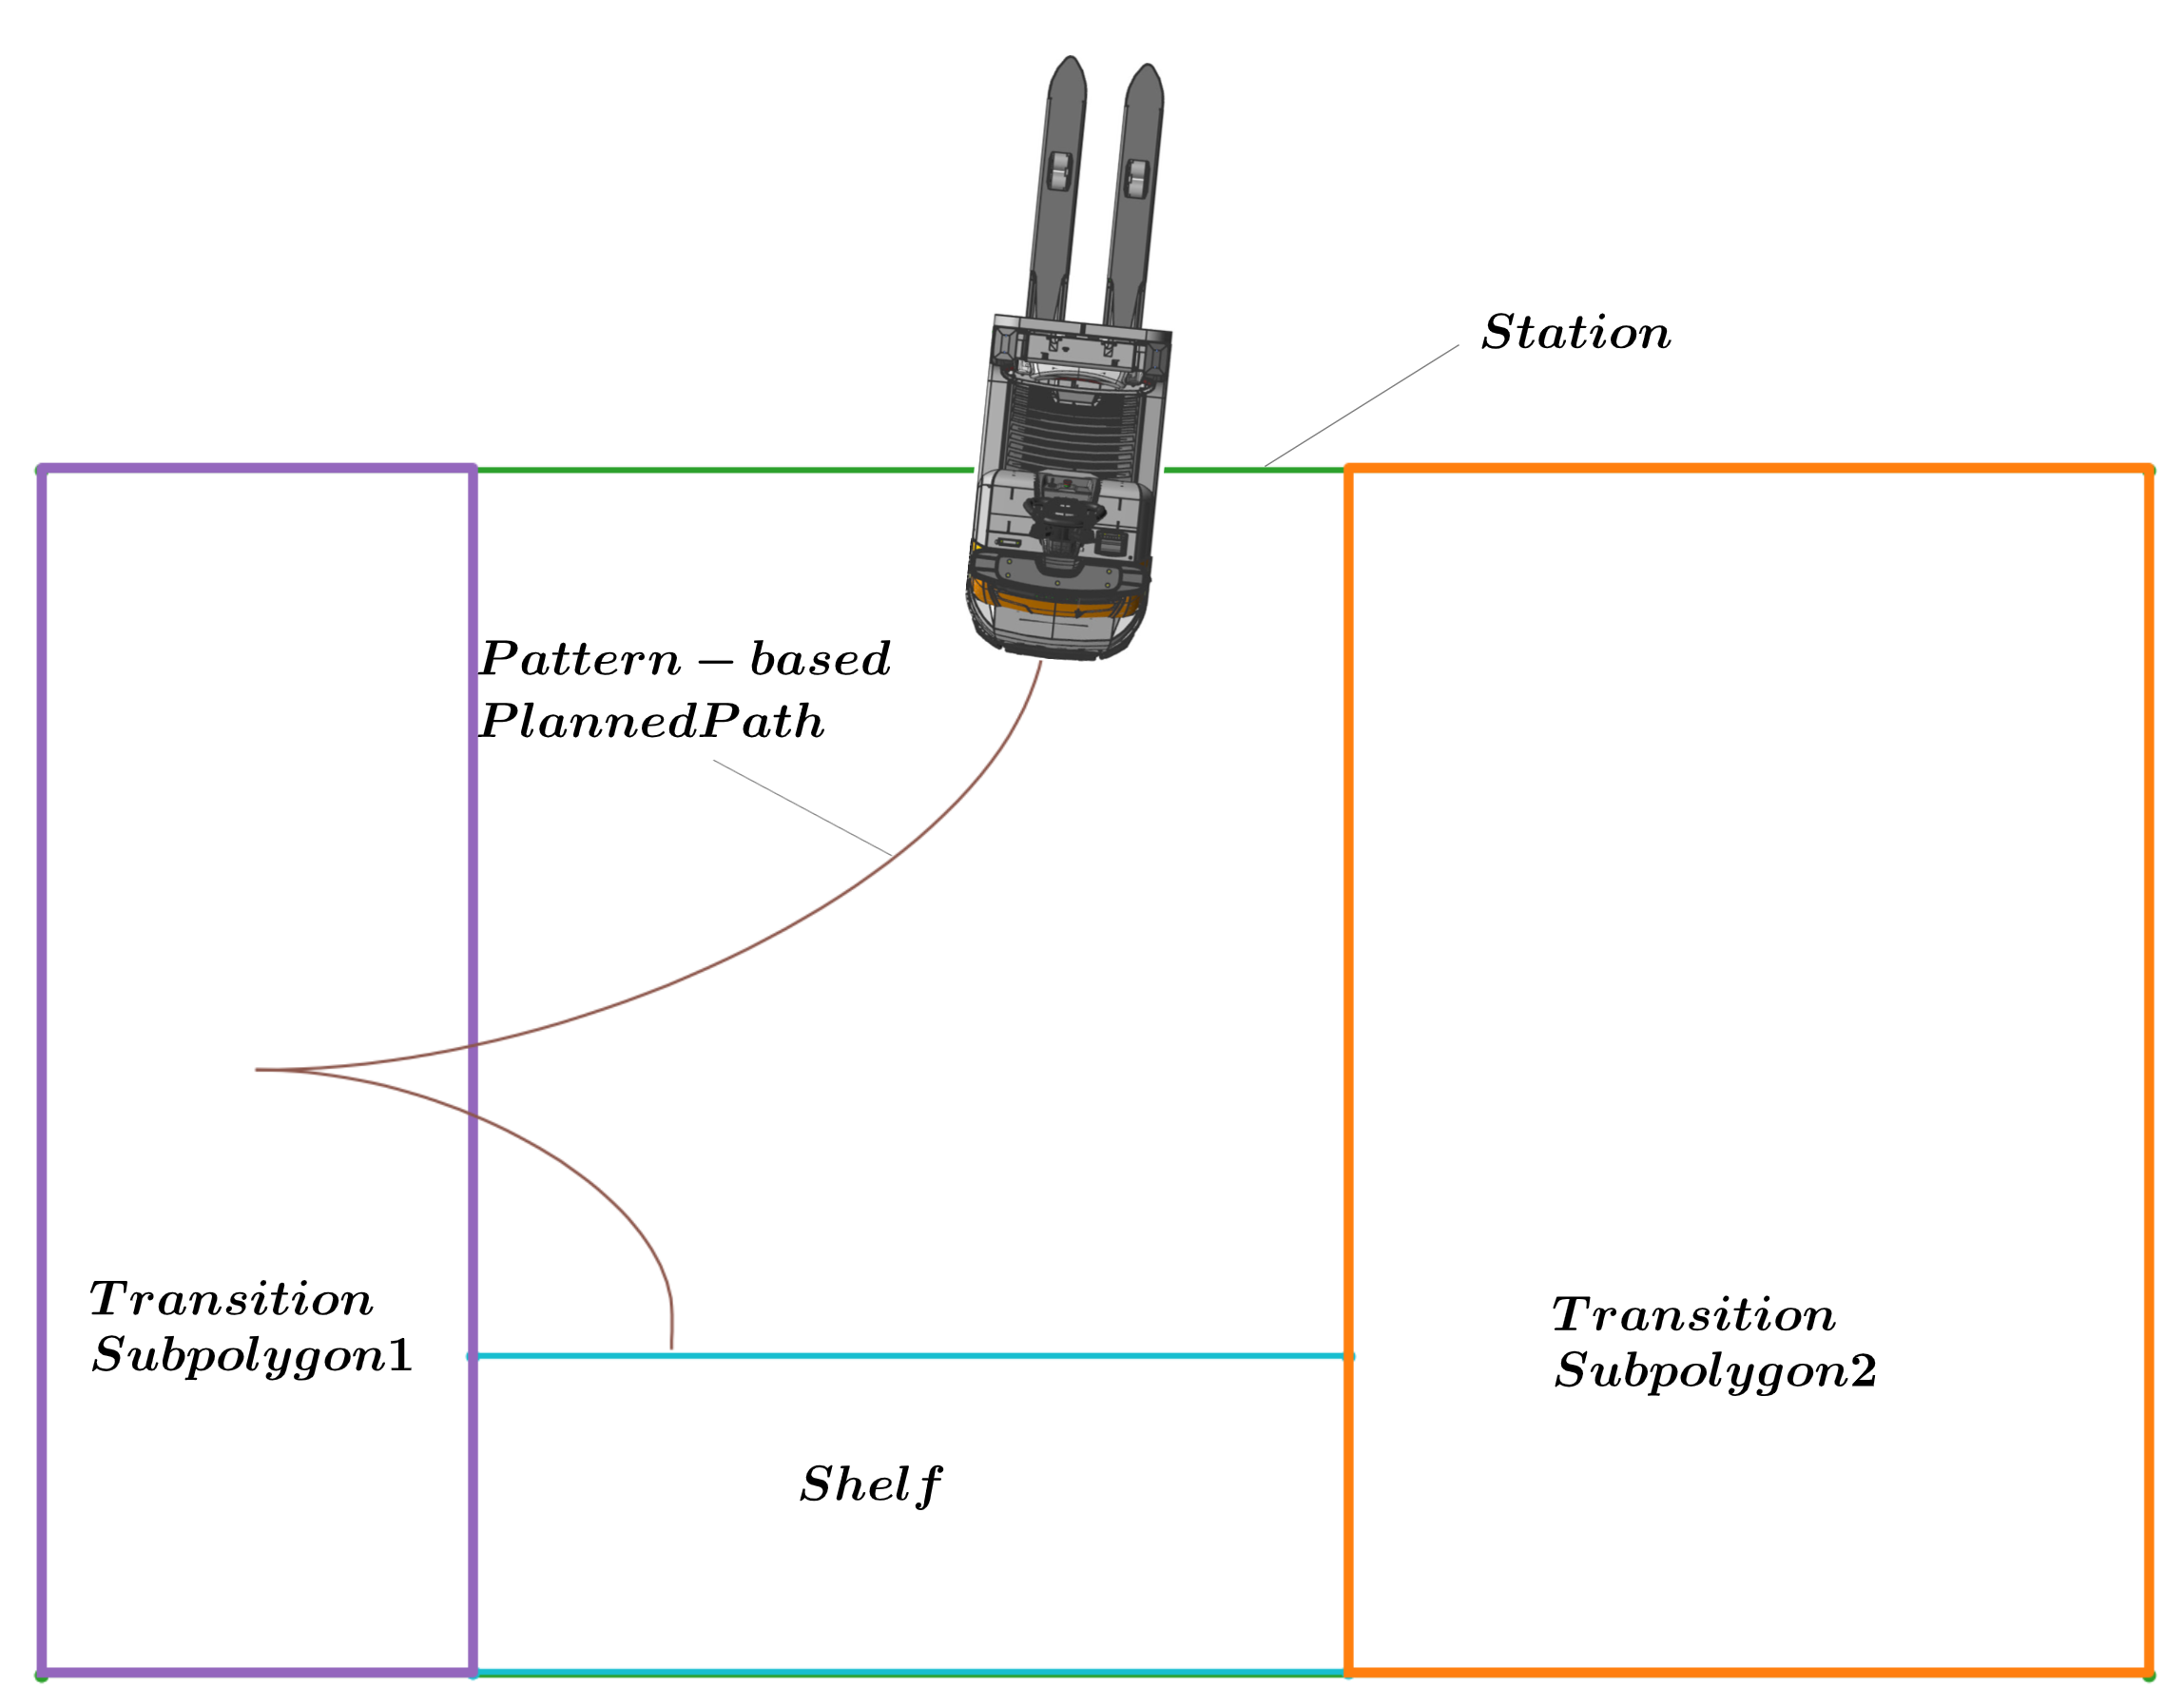
\includegraphics[width=3.5in]{images/Chap3/station2_pattern.png}
    \end{minipage}
    \caption{Test Results on Cloned Test Environment}
    \label{Test_clone}
\end{figure}

\begin{figure}[H]
    \centering
    \begin{subfigure}[b]{0.45\textwidth}
        \centering
        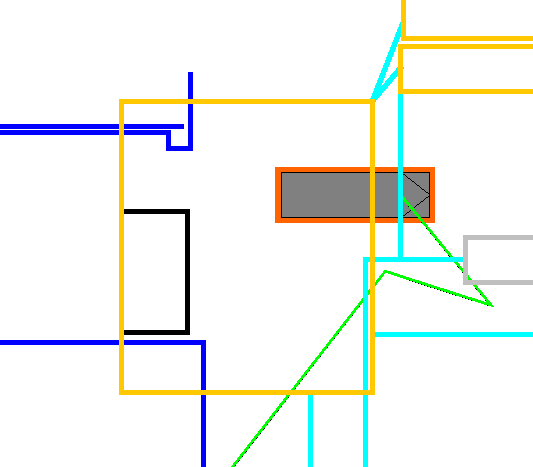
\includegraphics[width=\textwidth]{images/Chap3/Start_neksa.png}
        \caption{Test Results on the Simulated Environment: Truck at the start position}
        \label{fig:start}
    \end{subfigure}
    \hfill
    \begin{subfigure}[b]{0.45\textwidth}
        \centering
        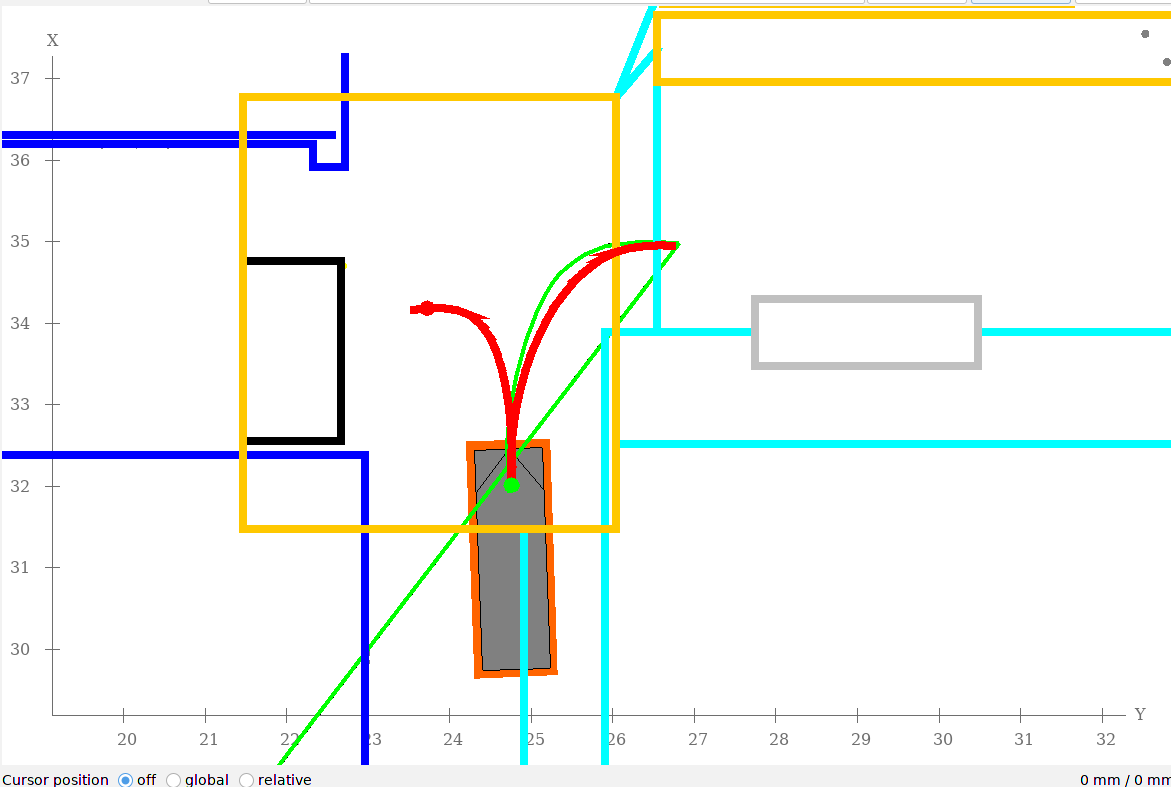
\includegraphics[width=\textwidth]{images/Chap2/Pattern_spline_simulation_3_driving.png}
        \caption{Test Results on the Simulated Environment: Truck driving the Spline-based Pattern path}
        \label{fig:spline}
    \end{subfigure}
    \caption{Test Results on the Simulated Environment}
    \label{TestResults}
\end{figure}

\begin{figure}[H]
    \centering
    \begin{minipage}{0.45\textwidth}
        \centering
        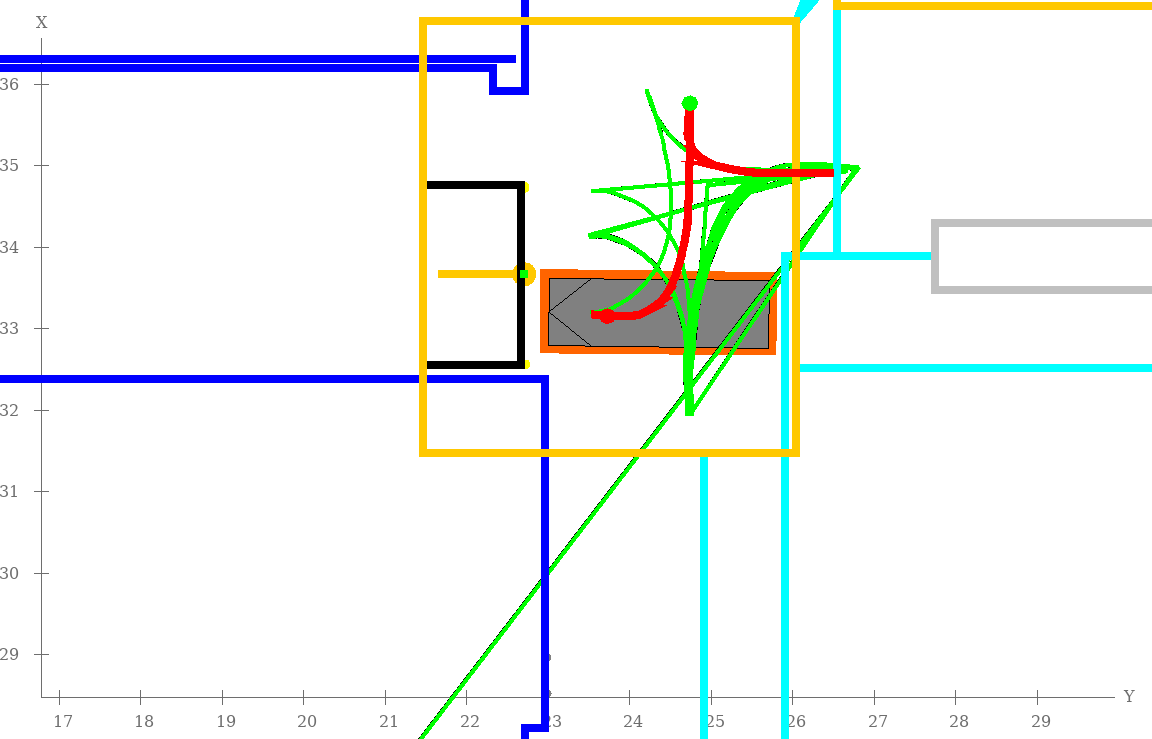
\includegraphics[width=\linewidth]{images/Chap2/Pattern_spline_simulation_1.png} % Replace with your figure
    \end{minipage}
    \begin{minipage}{0.45\textwidth}
        \centering
        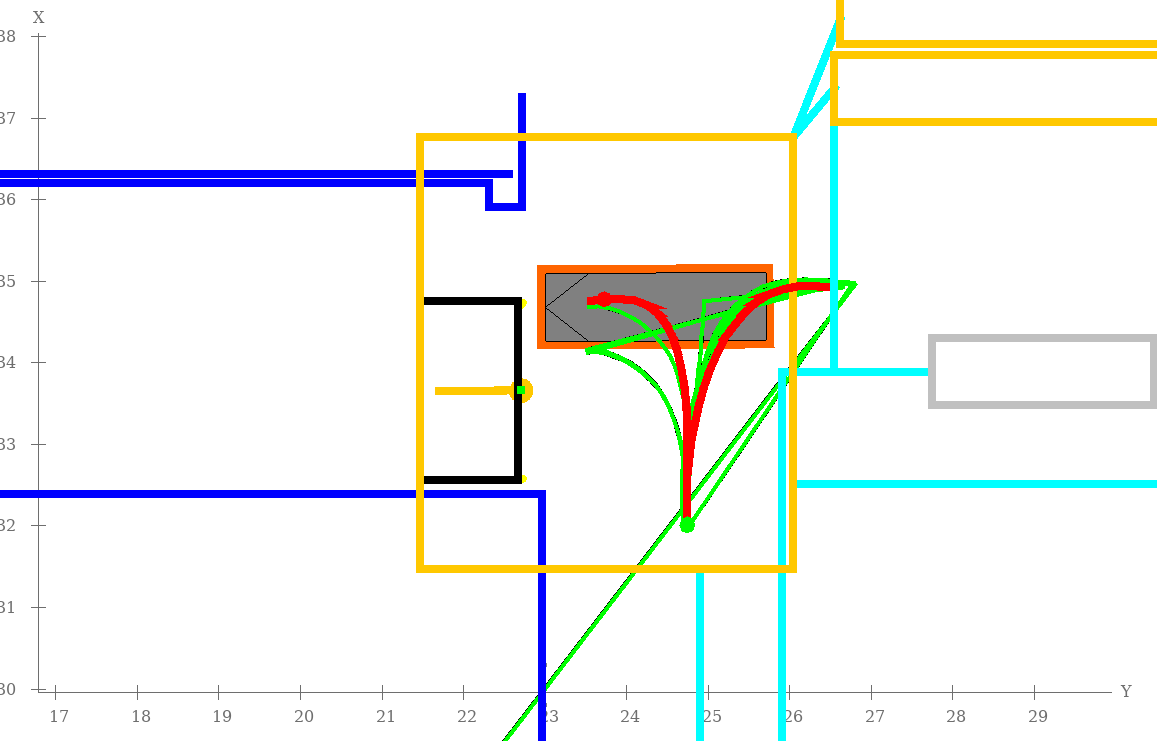
\includegraphics[width=\linewidth]{images/Chap2/Pattern_spline_simulation_2.png} % Replace with your figure
    \end{minipage}
    \caption{Test Results on the Simulated Environment: Truck at the Destination}
    \label{Test_Simu}
\end{figure}



\section{Path Evaluation Test Results and Validation}
In order to discriminate the Path Evaluation methods,
both approaches (3.3.2.1 and 3.3.2.2) were tested in the Independent Simulation Environment. 
Tests were ran on 10 different spline paths  that were generated with transition points scattered in 
the station \Ref{Mult_splines}.
Different locations of transition points were used to stress the metric outcomes by creating good and bad paths. 
The Exponential Weighted Path Evaluation was tested with \(\alpha\) = \(2\), \(\beta\) = \(0.0007\), 
\(\omega_c\)= \(0.7\) and \(\omega_L\)=\(0.3\).
The results are shown in figure \Ref{Test_Eval_Exp}: The bar chart reflects the Evaluation score of each 
spline path from figure \Ref{Mult_splines}. Each bar color reflects the same color spline.
The Normalized Weighted Path Evaluation was ran for two tests on the same splines set with:
\begin{itemize}
    \item \(\omega_c\)= \(0.7\) and \(\omega_L\)=\(0.3\)
    \item \(\omega_c\)= \(0.5\) and \(\omega_L\)=\(0.5\). 
\end{itemize}
 
The results are shown in figures \Ref{Test_Eval_Norm1} and \Ref{Test_Eval_Norm2}
%comment on results:

For the Exponential Weighted Path Evaluation, the results are correct. It is easy to differentiate poor-quality paths. 
For example, the Blue spline was used as the reference path, while the Orange, Gray, and Purple paths were intentionally 
created as bad paths. The Orange and Gray paths generate significant curvature near the destination, making it 
challenging for the vehicle to navigate and arrive in the correct position and orientation given the narrow aisle 
that it has to turn and navigate in as shown by figure  \Ref{curv_problem}. Given the high curvature and the proximity to the
destination, the truck decelerates and moves very slowly. Changes that it stops at the correct orientation 
that allows it to pickup the pallet are very low. Such path have to be avoided at all costs. The Purple path is longer 
and curved at the starting area. Furthermore, the Brown path demonstrates the best overall fitness. Although it is 
short, it introduces high curvatures at the transition and destination areas. Compared to the Blue and Red paths, 
the Brown path is shorter but less smooth. 
The Exponential Evaluation also favors the Dark Green path to the Pink one, even though the concentrated 
curvature at the end of the green path is high.
In conclusion, this evaluation method is very sensitive to path length and less 
sensitive to high concentrated curvatures. This is due to the high factor of the length term, in the range 
of thousands of millimeters, and the low factor of the curvature term which is around the magnitude of \(10^{-3}\).
It is inconvenient to change the factors \(\omega_c\) and \(\omega_L\) by increasing \(\omega_c\) and 
decreasing \(\omega_L\) as the difference becomes huge while it is mandatory to attribute 
importance to both factors. Besides, this Metric is very sensitive to the change of the \(\alpha\) and \(\beta\) factors.
These factors must be carefully tuned to fit all use cases and account for varying station sizes and configurations. 
However, finding factors that are scalable across different use cases is not straightforward.

\noindent On the other hand, The Normalized Weighted Path Evaluation, chose the Red path as the best fitness, 
outperforming the Blue pattern path. This is due to the remarkable less curvature of the Red path at the start 
and transition locations due to its proximity to the transition polygon and distance to the destination.
These factors allow for smooth driving along the path.
Comparing figures \Ref{Test_Eval_Norm1} and \Ref{Test_Eval_Norm2}, the approach of outweighing the curvature 
over the length outperforms the equal weights approach. The Pink path is visibly better than the Brown due 
to better smoothness and the first weights approach discriminates them better. 
Given the challenges associated with driving along smooth paths, it is a strategic decision to prioritize the 
curvature term over the length term. Navigating a slightly longer path is far less difficult than handling a path 
with sharp curves.
This approach is not affected by the difference of range between length and curvature metrics given that 
they are each divided respectively by the reference path's length and curvature. This not only balances out the 
two terms but also makes it fit all use cases and account for varying station sizes and configurations given that 
the reference path is always relevnat to the present station.

As a final point, \textbf{the selected approach is the Normalized Weighted Path Evaluation} with \(\omega_c\)= \(0.7\) 
and \(\omega_L\)=\(0.3\) given by equation \Ref{Norm_function}.

The Path Evaluation Approach is validated and can be used for the path Optimization phase.
The approach was validated for the following reasons: 
\begin{itemize}
    \item The Selected Evaluation method satisfies the goal of optimizing path length and thus travel time
    and limiting high curvature and challenging turns of the bulky truck by optimizing curvature change.
    \item Using the Evaluation Method, good and poor quality pattern paths can be discriminated by 
    affecting a score to each path according to its properties and comparing them.
\end{itemize}

The approach is ready to be used as the cost function of the optimizer.

\begin{figure}[H]
    \begin{center}
        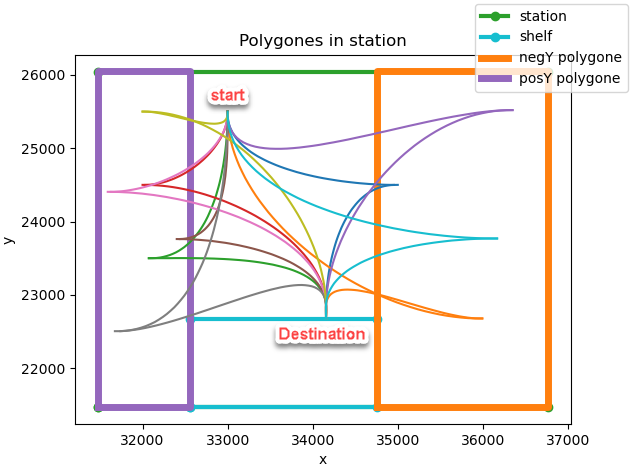
\includegraphics[width=4in]{images/Chap2/Mult_Splines_noted.png} % Replace with your figure
        \caption{Test Results on the Simulated Environment: Multiple Splines Visualization}
        \label{Mult_splines}
        \end{center}    
\end{figure}

\begin{figure}[H]
    \begin{center}
        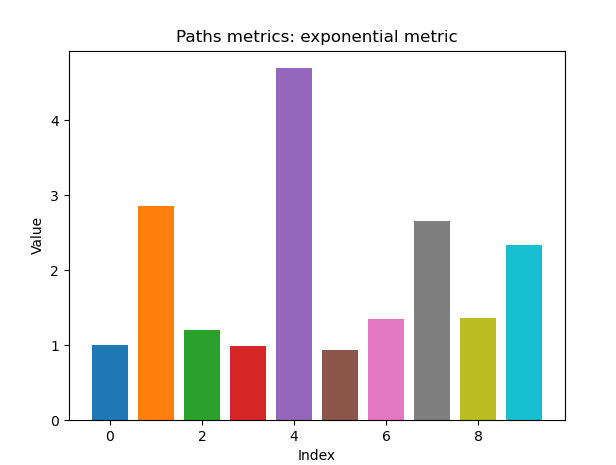
\includegraphics[width=4in]{images/Chap2/Exp_Results.png} % Replace with your figure
        \caption{Test Results on the Simulated Environment: Evaluation results of the Exponential Approach}
        \label{Test_Eval_Exp}
        \end{center}    
\end{figure}

\begin{figure}[H]
    \begin{center}
        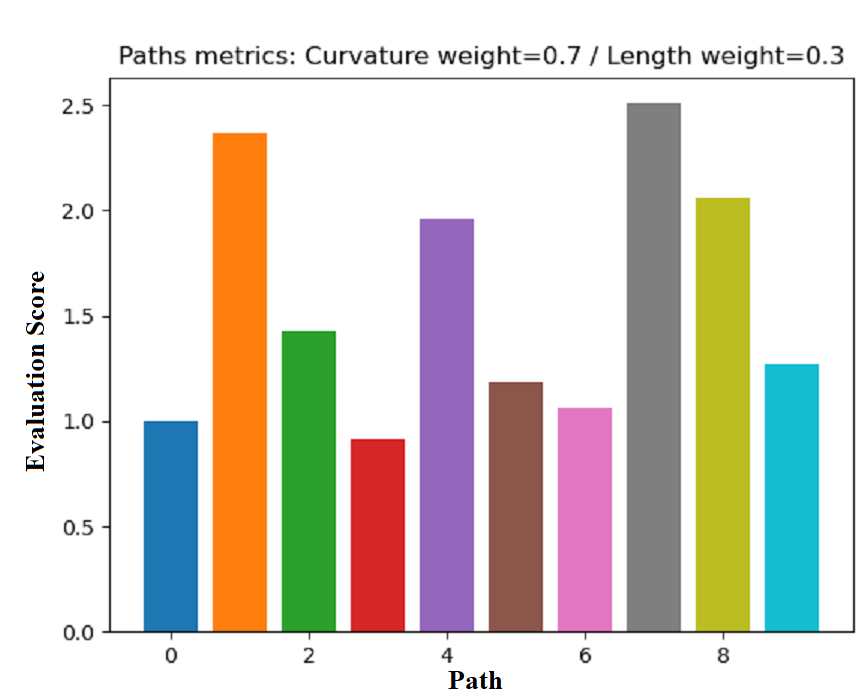
\includegraphics[width=4in]{images/Chap2/w_0.7.png} % Replace with your figure
        \caption{Test Results on the Simulated Environment: Evaluation results of the Normalized Approach
        with weighing out the curvature}
        \label{Test_Eval_Norm1}
        \end{center}    
\end{figure}
\begin{figure}[H]
    \begin{center}
        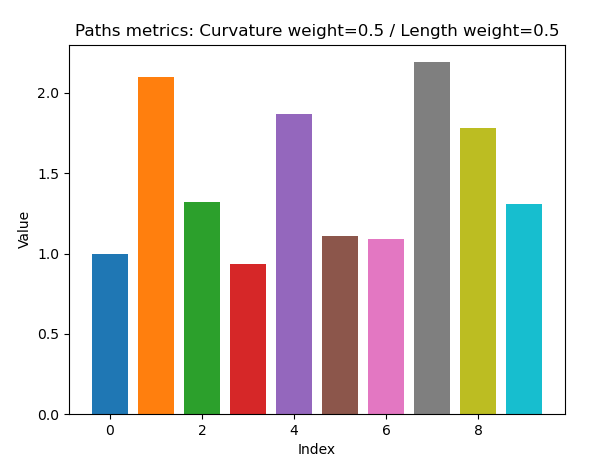
\includegraphics[width=4in]{images/Chap2/w_0.5.png} % Replace with your figure
        \caption{Test Results on the Simulated Environment: Evaluation results of the Normalized Approach
        with equal weights}
        \label{Test_Eval_Norm2}
        \end{center}    
\end{figure}

\begin{figure}[H]
    \begin{center}
        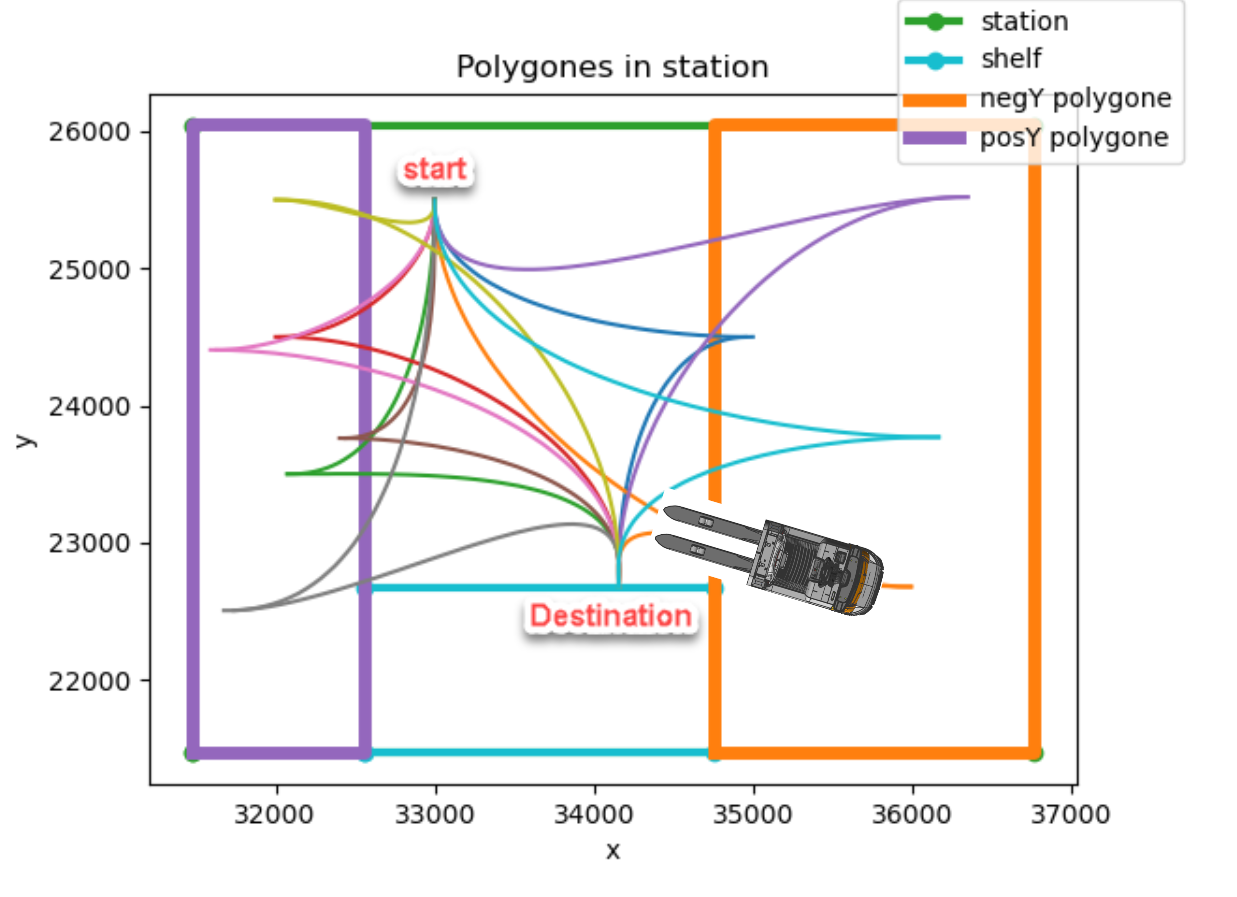
\includegraphics[width=4in]{images/Chap2/curv_problem.png} % Replace with your figure
        \caption{Navigating high curvatures in narrow areas}
        \label{curv_problem}
        \end{center}    
\end{figure}

\section{Path Optimization Test Results and Validation}

Using the Path Creation and the Selected Evaluation approach, the optimization approach is tested.
First the Optimizer is tested in an empty station, then it is tested against obstacles placed inside the station 
in different locations. 
The optimization algorithm is ran first on The 
Independent Simulation Environment to verify the relevance of the optimization approach to the pattern-based 
path. 
For this test, The Optimizer evaluates 10 generations of 10 paths for each subpolygon, it calculates the fitness value 
for each path and saves the overall best fitness value from both subpolygons. 
Figure \Ref{OptResult1} shows the result inside the Independent Simulation Environment for a station empty of obstacles:
The figure illustrates the candidate paths of the first of the 10 generations, along with the optimum paths from 
both subpolygons in bold Red and Brown "champion paths" as called in the algorithm. 
The algorithm successfully rejects poor quality paths like the lowest right red path which has two direction changes 
along the path due to the sharp turn in the beginning, and the highest left blue path that 
has an unfeasible sharp turn at the target.
The approach is validated at this stage. 

\begin{figure}[H]
    \begin{center}
        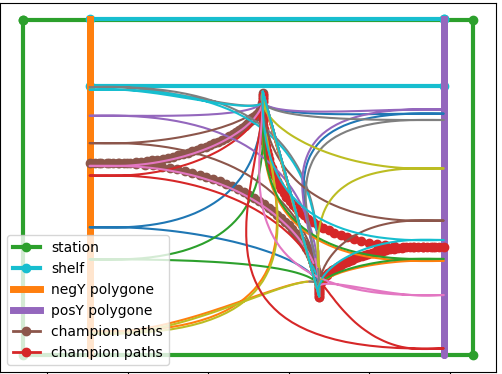
\includegraphics[width=4in]{images/Chap3/Gen1_crop.png} % Replace with your figure
        \caption{Optimizer results in empty station of one of 10 generations with the overall best paths 
        visualized in bold red and brown}
        \label{OptResult1}
        \end{center}    
\end{figure}


The second test is ran with obstacles placed in different positions in the station. 
The Algorithm results on figure \Ref{OptResult2} illustrate that the optimizer is capable of generating paths the avoid 
obstacles. The optimizer does generate paths that cross the quadrilateral obstacle but those paths 
are eliminated by better quality paths: the optimum paths in Brown. The quadrilateral obstacle was placed 
in a critical area, the center of the station to stress the optimizer. On the other hand, 
the rectangle obstacle was placed in the right corner of the station at a far distance from the start position,
the optimal transition area inside the subpolygon, and the target.
Although the two paths are  correct, the brown path is highly curved at the beginning because it avoids the 
quadrilateral obstacle. However, the red path is smoother at the start and destination segments of the path.

\begin{figure}[H]
    \begin{center}
        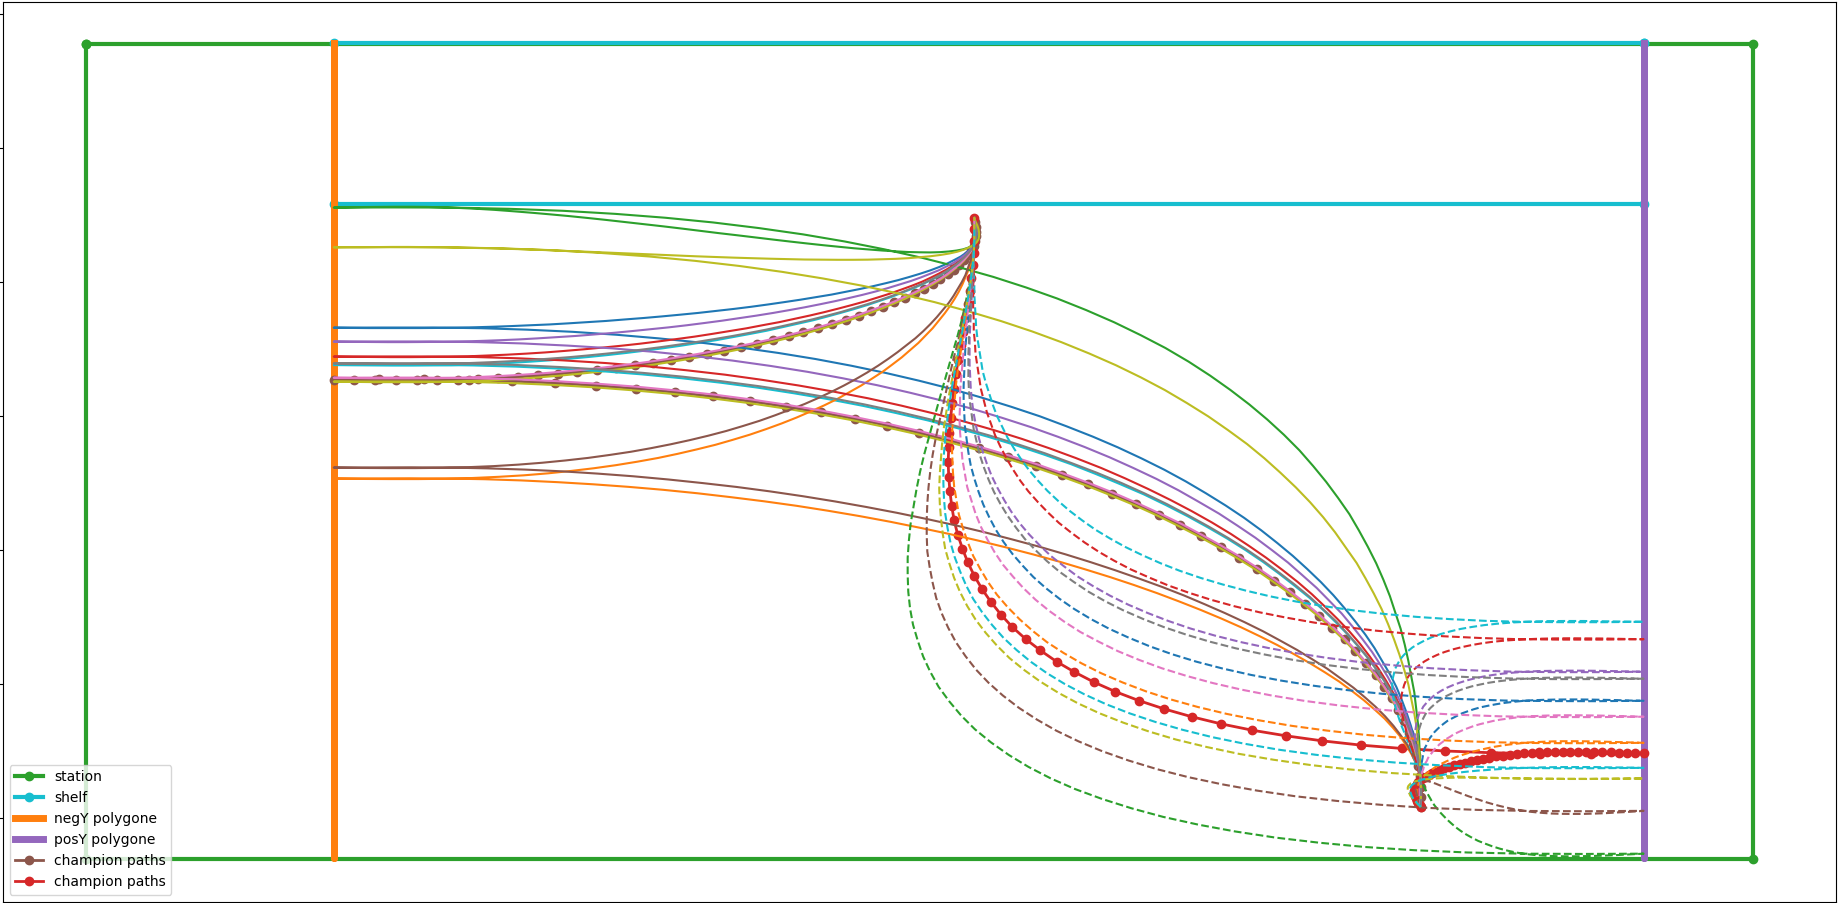
\includegraphics[width=5in]{images/Chap3/scenario3_crop.png} % Replace with your figure
        \caption{Optimizer results in presence of obstacles of one of 10 generations with the overall best paths 
        visualized in bold red and brown}
        \label{OptResult2}
        \end{center}    
\end{figure}

Another obstacle situation was tested and illustrated by figure \Ref{OptResult3}.
The obstacles in this situation were placed in the center of the station . 
For this case the regular optimizer was unable to find a solution that does not collide 
with the obstacles. However, by increasing the number of the waypoints (approach in section 3.4.2.1),
The optimizer was effective in finding collision free paths. 


\begin{figure}[H]
    \begin{center}
        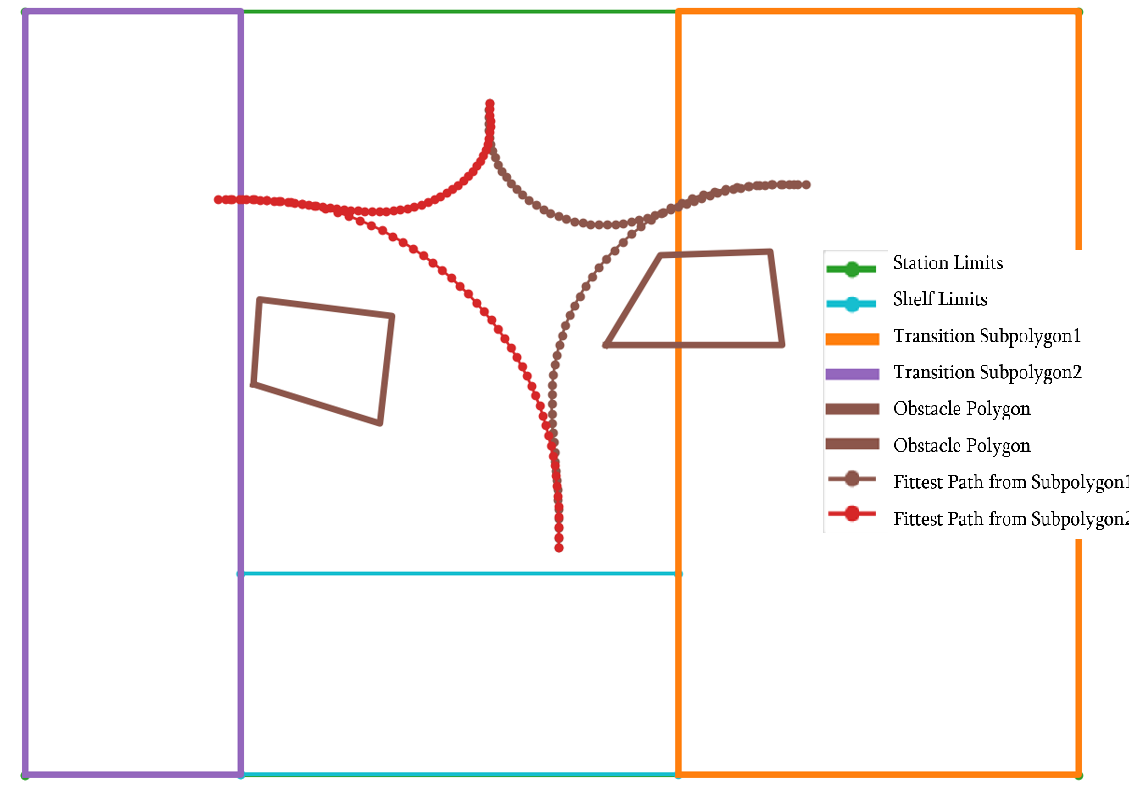
\includegraphics[width=4in]{images/Chap3/Figure_6.png} % Replace with your figure
        \caption{Optimizer results in presence of obstacles and influence of increasing path waypoints}
        \label{OptResult3}
        \end{center}    
\end{figure}

The approach is validated for a moderate complexity environment.

Given that the approach was validated in the Independent Simulation Environment, the tests are 
ran on the RACK Simulation Environment. Two test scenarios are created: 
The first is called the \(Simple~Environment\) which is an obstacle-free station and the second is
called the \(Complex~Environment\) where an obstacle is placed in one side of the station. 
In reality, the \(Simple~Environment\) is not simple because the sensors detect the warehouse walls,
shelves, objects, and other vehicles, but the station area is free of stranger objects.
The test in the \(Simple~Environment\) illustrated by figure \Ref{OptResult4} was done by placing the 
AMR in the simulation in the starting position (green rectangle) and selecting the target position on 
the simulation model. The expected target position is the red rectangle. 
The path is planned following the pattern and links the AMR from its start position to the target position.
The blueprints along the path represent the positions that the AMR will be at when driving the path.
The footprint helps to ensure that the AMR will not collide with surrounding objects and 
validate the optimizer's ability to avoid obstacles. 

\begin{figure}[H]
    \begin{center}
        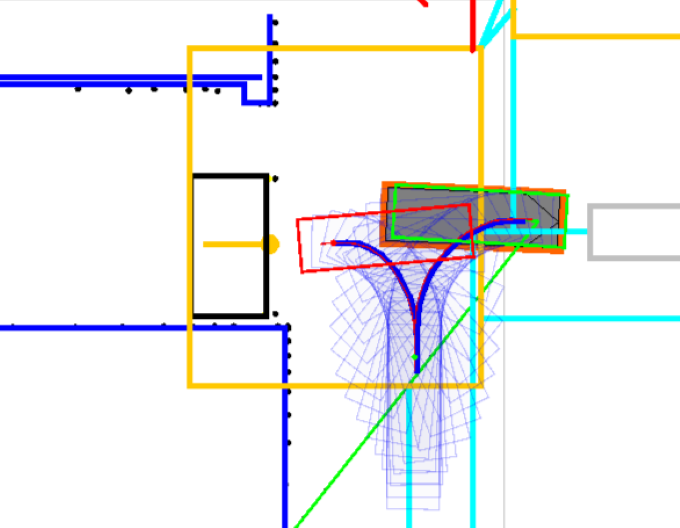
\includegraphics[width=4in]{images/Chap3/Start.png} % Replace with your figure
        \caption{Optimizer results in a simple environment tested inside the RACK simulation: Start Position}
        \label{OptResult4}
        \end{center}    
\end{figure}

\begin{figure}[H]
    \begin{center}
        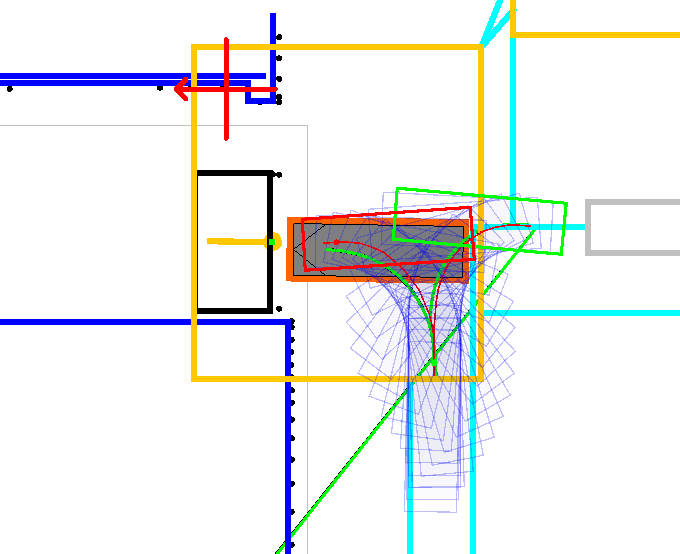
\includegraphics[width=4in]{images/Chap3/Target.png} % Replace with your figure
        \caption{Optimizer results in a simple environment tested inside the RACK simulation: Target Position}
        \label{OptResult5}
        \end{center}    
\end{figure}

As for the \(Complex~Environment\), an obstacle was placed at the side of the station 
blocking one of the subpolygons as illustrated in figure \Ref{OptResult6}: the blue rectangle at the bottom 
of the figure.
The planned pattern path (red path) transitions in the opposite subpolygon as it is clear of obstacles.
The optimizer successfully generates a pattern path that avoids known obstacles such as the shelf and 
the warehouse walls as well as new obstacles like the blue rectangle. 
The generated path is aligned with the kinematic constraints of the vehicle as illustrated on figure \Ref{OptResult7}: 
it avoids highly curved turns and limits the direction changes to one thus ensuring a smooth navigation.
Finally, the truck docks the target location at the desired position as shown in figure \Ref{OptResult8}: 
The forks are facing the shelf and ready to start pick up/ drop process. 

\textbf{Remark}: the shift of the final position of the vehicle on figure \Ref{OptResult8} is due 
to control issues. Currently, the path following is not completely correct and requires 
control improvement.

\begin{figure}[H]
    \begin{center}
        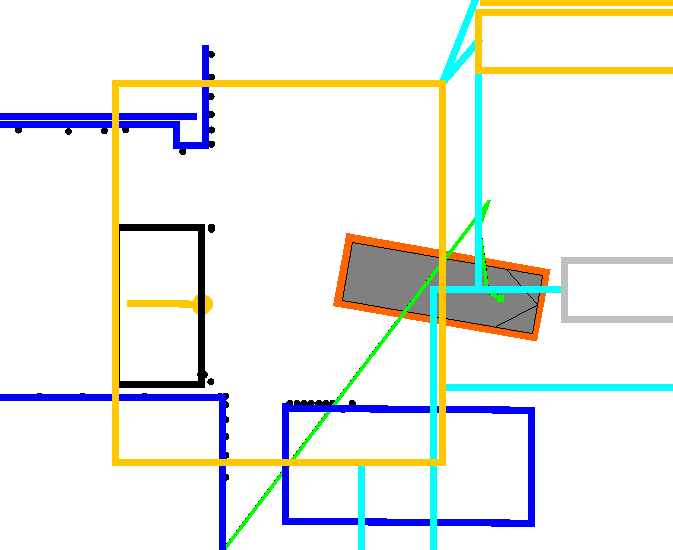
\includegraphics[width=4in]{images/Chap3/4.png} % Replace with your figure
        \caption{Optimizer results in a Complex environment tested inside the RACK simulation: Start Position}
        \label{OptResult6}
        \end{center}    
\end{figure}

\begin{figure}[H]
    \begin{center}
        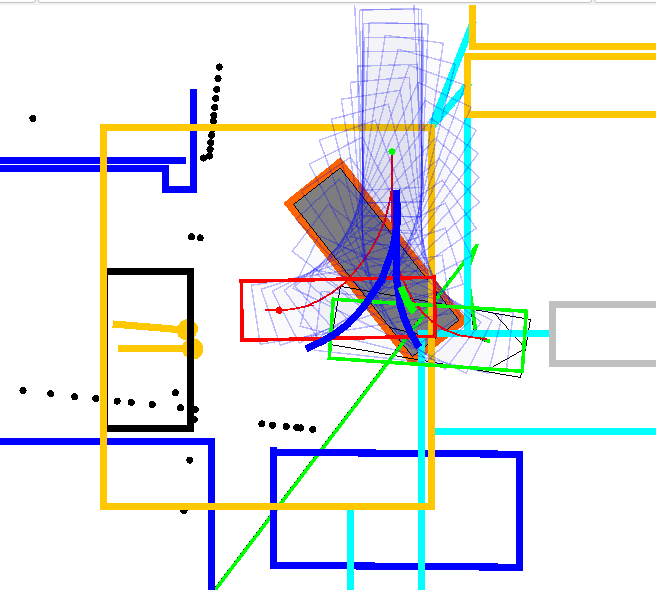
\includegraphics[width=4in]{images/Chap3/2.png} % Replace with your figure
        \caption{Optimizer results in a Complex environment tested inside the RACK simulation: AMR Navigating the path}
        \label{OptResult7}
        \end{center}    
\end{figure}

\begin{figure}[H]
    \begin{center}
        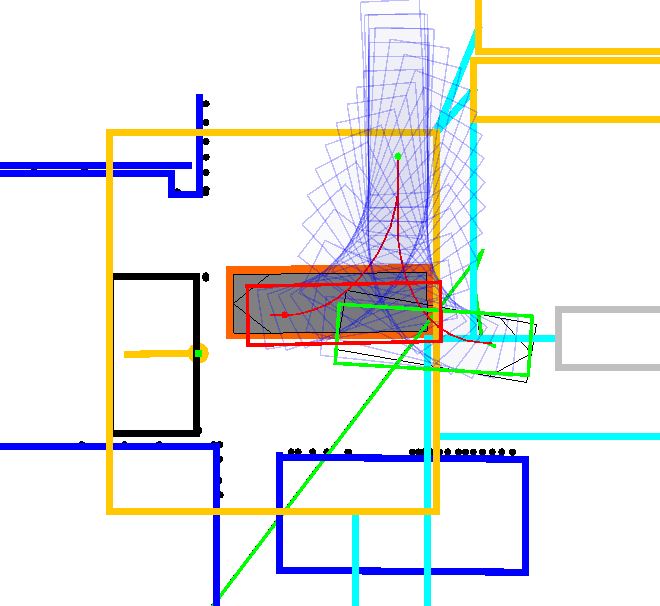
\includegraphics[width=4in]{images/Chap3/3.png} % Replace with your figure
        \caption{Optimizer results in a Complex environment tested inside the RACK simulation: Target Position}
        \label{OptResult8}
        \end{center}    
\end{figure}

Using the \(Simple~Environment\) and the \(Complex~Environment\) tests were ran inside the 
RACK Simulation Environment to compare the performance of the Metaheuristic Algorithms: GA, DE, PSO,
ACO, and SA. 

The same starting and Target Positions were used for each scenario. For the \(Complex~\\Environment\),
the same obstacle was used for all the algorithm tests to create the same test conditions, the obstacle used is 
marked in green on figure \Ref{OptResult9}. All algorithms were configured to evolve around 200 candidates.
The comparison between the Algorithms in the simulation is based on: 
\begin{itemize}
    \item The Planning Time: the time that each algorithm takes to evolve a solution.
    \item The Created Path's Fitness Values.
\end{itemize}

Table \Ref{tab:planning_time} shows the planning times for simple and complex Environment 
for each algorithm. 
For the Simple Environment, the DE algorithm prevails at a planning time of \(27ms\).
The worst planning time is with the SA algorithm at \(80ms\). 
GA, PSO, and ACO have the same range of Planning time \(56\) to \(59ms\).
For the complex Environment, The raking is the same: the best algorithm in terms of planning time 
is the DE at \(44ms\), next comes the ACO at \(65ms\). The least performing algorithm remains the SA 
with a planning time of \(78ms\). It is noticeable that the planning time increased overall
for almost all the algorithms in the complex environment scenario. 
This is due to the checking of the scan points that increase as more objects are introduced around the AMR.

Using the planning time based comparison the DE algorithm is the most performing in terms of planning time. 

Table \Ref{tab:fitness_values} details the fitness values for both scenarios. It is worth mentioning
that the obstacle is placed inside subpolygon1 in this case.
For the Simple Environment, the GA was able to find the fittest candidate at an evaluation score of 
\(0.32\) in subpolygon2, however, the DE has the highest fitness values \(0.652\) in subpolygon1 and \(0.56\) in subpolygon2 
even though it was the fastest in terms of planning time.
For the complex Environment, the PSO was the fittest with an evaluation score of \(0.38\) in subpolygon2 and very 
close was the DE with \(0.384\). As for subpolygon1 where the obstacle stands, the fitness values are very high.
The values can be clustered into two groups:
\begin{itemize}
    \item Knockout value: this is the cluster of the fitness values equal to \(50\). It was obtained
    with the ACO and DE. The knockout value is the fitness value assigned to the paths that collide with obstacles.
    Returning a fitness function of \(50\) means that the optimizer was not able to find a path at that subpolygon.
    \item High values < \(50\): For GA, PSO, and SA the fitness values are respectively \(31\), \(1.159\), and \(1.258\).
    These values are caused by penalizing the high curvatures.
    If a path's maximum curvature exceeds the maximum tolerated curvature of the truck, the Path gets penalized by 
    emphasizing it curvature. Despite the poor quality of the paths, these algorithms still found feasible solutions 
    to get around the obstacle. 
\end{itemize}

Using this comparison, the PSO algorithm outperforms the other algorithms in complex environments as it 
finds the fittest path which refers to the shortest path and the least curvature change and also finds a path in 
the constrained subpolygon where the obstacle stands.

\begin{figure}[H]
    \begin{center}
        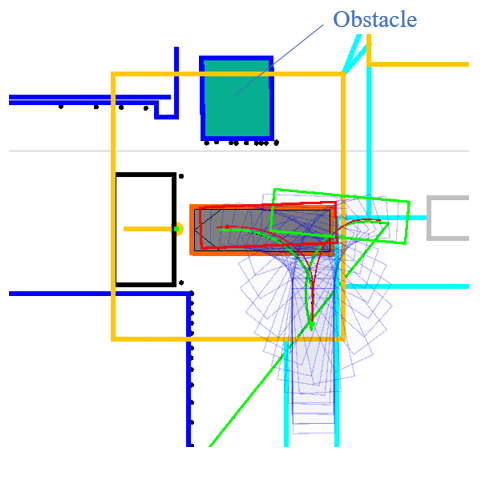
\includegraphics[width=4in]{images/Chap3/obstacle_complicated.png} % Replace with your figure
        \caption{Obstacle Used for Metaheuristic Algorithms comparison in the complex scenario}
        \label{OptResult9}
        \end{center}    
\end{figure}

\begin{table}[H]
    \centering
    \caption{Comparison of Planning Time for Different Algorithms in Simple and Complex Environments (in milliseconds)}

    \resizebox{\textwidth}{!}{%
    \begin{tabular}{|p{3.5cm}|p{5cm}|p{5cm}|}
    \hline
    \textbf{Algorithm} & \textbf{Planning Time (Simple Environment) (ms)} & \textbf{Planning Time (Complex Environment) (ms)} \\
    \hline
    Genetic Algorithm & 57 & 73 \\
    \hline
    Particle Swarm Optimization & 59 & 67 \\
    \hline
    Ant Colony Optimization & 56 & 65 \\
    \hline
    Simulated Annealing & 80 & 78 \\
    \hline
    \rowcolor{green!30} Differential Evolution & 27 & 44 \\
    \hline
    \end{tabular}%
    }
    \label{tab:planning_time}
\end{table}

\begin{table}[H]
    \centering
    \caption{Comparison of Fitness Values of the optimum paths generated by Different Algorithms in Simple and Complex Environments}

    \resizebox{\textwidth}{!}{%
    \begin{tabular}{|p{4cm}|p{2.5cm}|p{2.5cm}|p{2.5cm}|p{2.5cm}|}
    \hline
    \multirow{2}{*}{\textbf{Algorithm}} & \multicolumn{2}{c|}{\textbf{Simple Environment}} & \multicolumn{2}{c|}{\textbf{Complex Environment}} \\
    \cline{2-5}
     & \textbf{Subpolygon1 Fitness} & \textbf{Subpolygon2 Fitness} & \textbf{Subpolygon1 Fitness} & \textbf{Subpolygon2 Fitness} \\
    \hline
    Genetic Algorithm       & \cellcolor{green!30} 0.549  & \cellcolor{green!30} 0.32  & 31.0  & 0.449 \\
    \hline
    Particle Swarm Optimization  & 0.561  & 0.349  & \cellcolor{green!30} 1.159  & \cellcolor{green!30} 0.38 \\
    \hline
    Ant Colony Optimization      & 0.542  & 0.384  & 50.0  & 0.417 \\
    \hline
    Simulated Annealing     & 0.45  & 0.394  & 1.258  & 0.428 \\
    \hline
    Differential Evolution  & 0.652  & 0.56  & 50.0  & 0,384 \\
    \hline
    \end{tabular}%
    }
    \label{tab:fitness_values}    
\end{table}

\section{Field-Testing of the Solution on the AMR}
This section sums up the developed module for a field test on the iGo Neo Truck. 
First the test Conditions are outlined, then the planning process with the sensor input are explained.
Finally, the planned path and navigation of the truck in each scenario are discussed.

The Approach is tested in 3 different scenarios:
\begin{itemize}
    \item A Simple Test Environment where The station is free of obstacles.
    \item Moderate complexity Test Environments where  obstacles are placed in 2 areas of the station:
    left and right sides of the shelf. The obstacles are intended to block one subpolygon.
\end{itemize}

\subsection{Simple Test Environment}
The truck was placed at position \(x = 33026\), \(y = 28070\), and \(\rho = 100.0^\circ\) 
as illustrated by 
figure \Ref{OptResult10}.
The sensor input of the truck as scan points which detects the obstacles is represented by black points
on the figure. Figure \Ref{OptResult11} shows the start position of the Truck inside the warehouse.
The RACK simulation is now a real-time visualization of the real warehouse.
The goal is to dock the shelf which is represented in the real warehouse image \Ref{OptResult11}
by the yellow floor anchors at position \(x = 33426\), \(y = 22696\), and \(\rho = 0.0^\circ\). 
They hold the reflectors that return the shelf's position.
After station, shelf and target recognition, and station partitioning,
the optimizer starts generating and evaluating the candidate paths.
After successful processing of an optimum path, the truck start driving it.
The optimum path is illustrated on figure \Ref{OptResult50} in red. The path is followed by the truck 
that moves in opposite direction and negative speed until the transition location.
Starting from the transition location, it drives in main direction orienting the forks 
towards the shelf in preparation to dock then pickup or drop. 


\begin{figure}[H]
    \begin{center}
        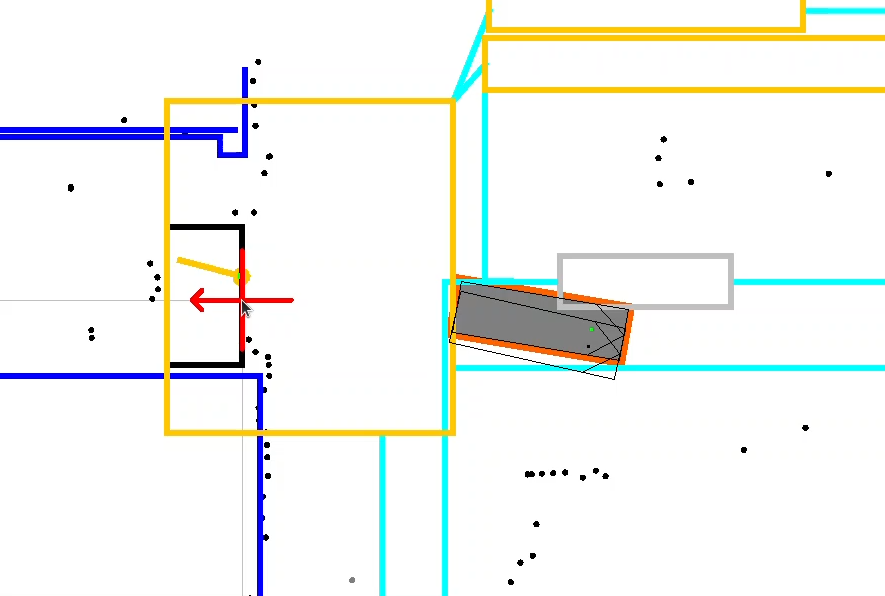
\includegraphics[width=4in]{images/Chap3/StartSimpleEnv.png} % Replace with your figure
        \caption{Environment and Start position of the Simple Test Scenario}
        \label{OptResult10}
        \end{center}    
\end{figure}


\begin{figure}[H]
    \begin{center}
        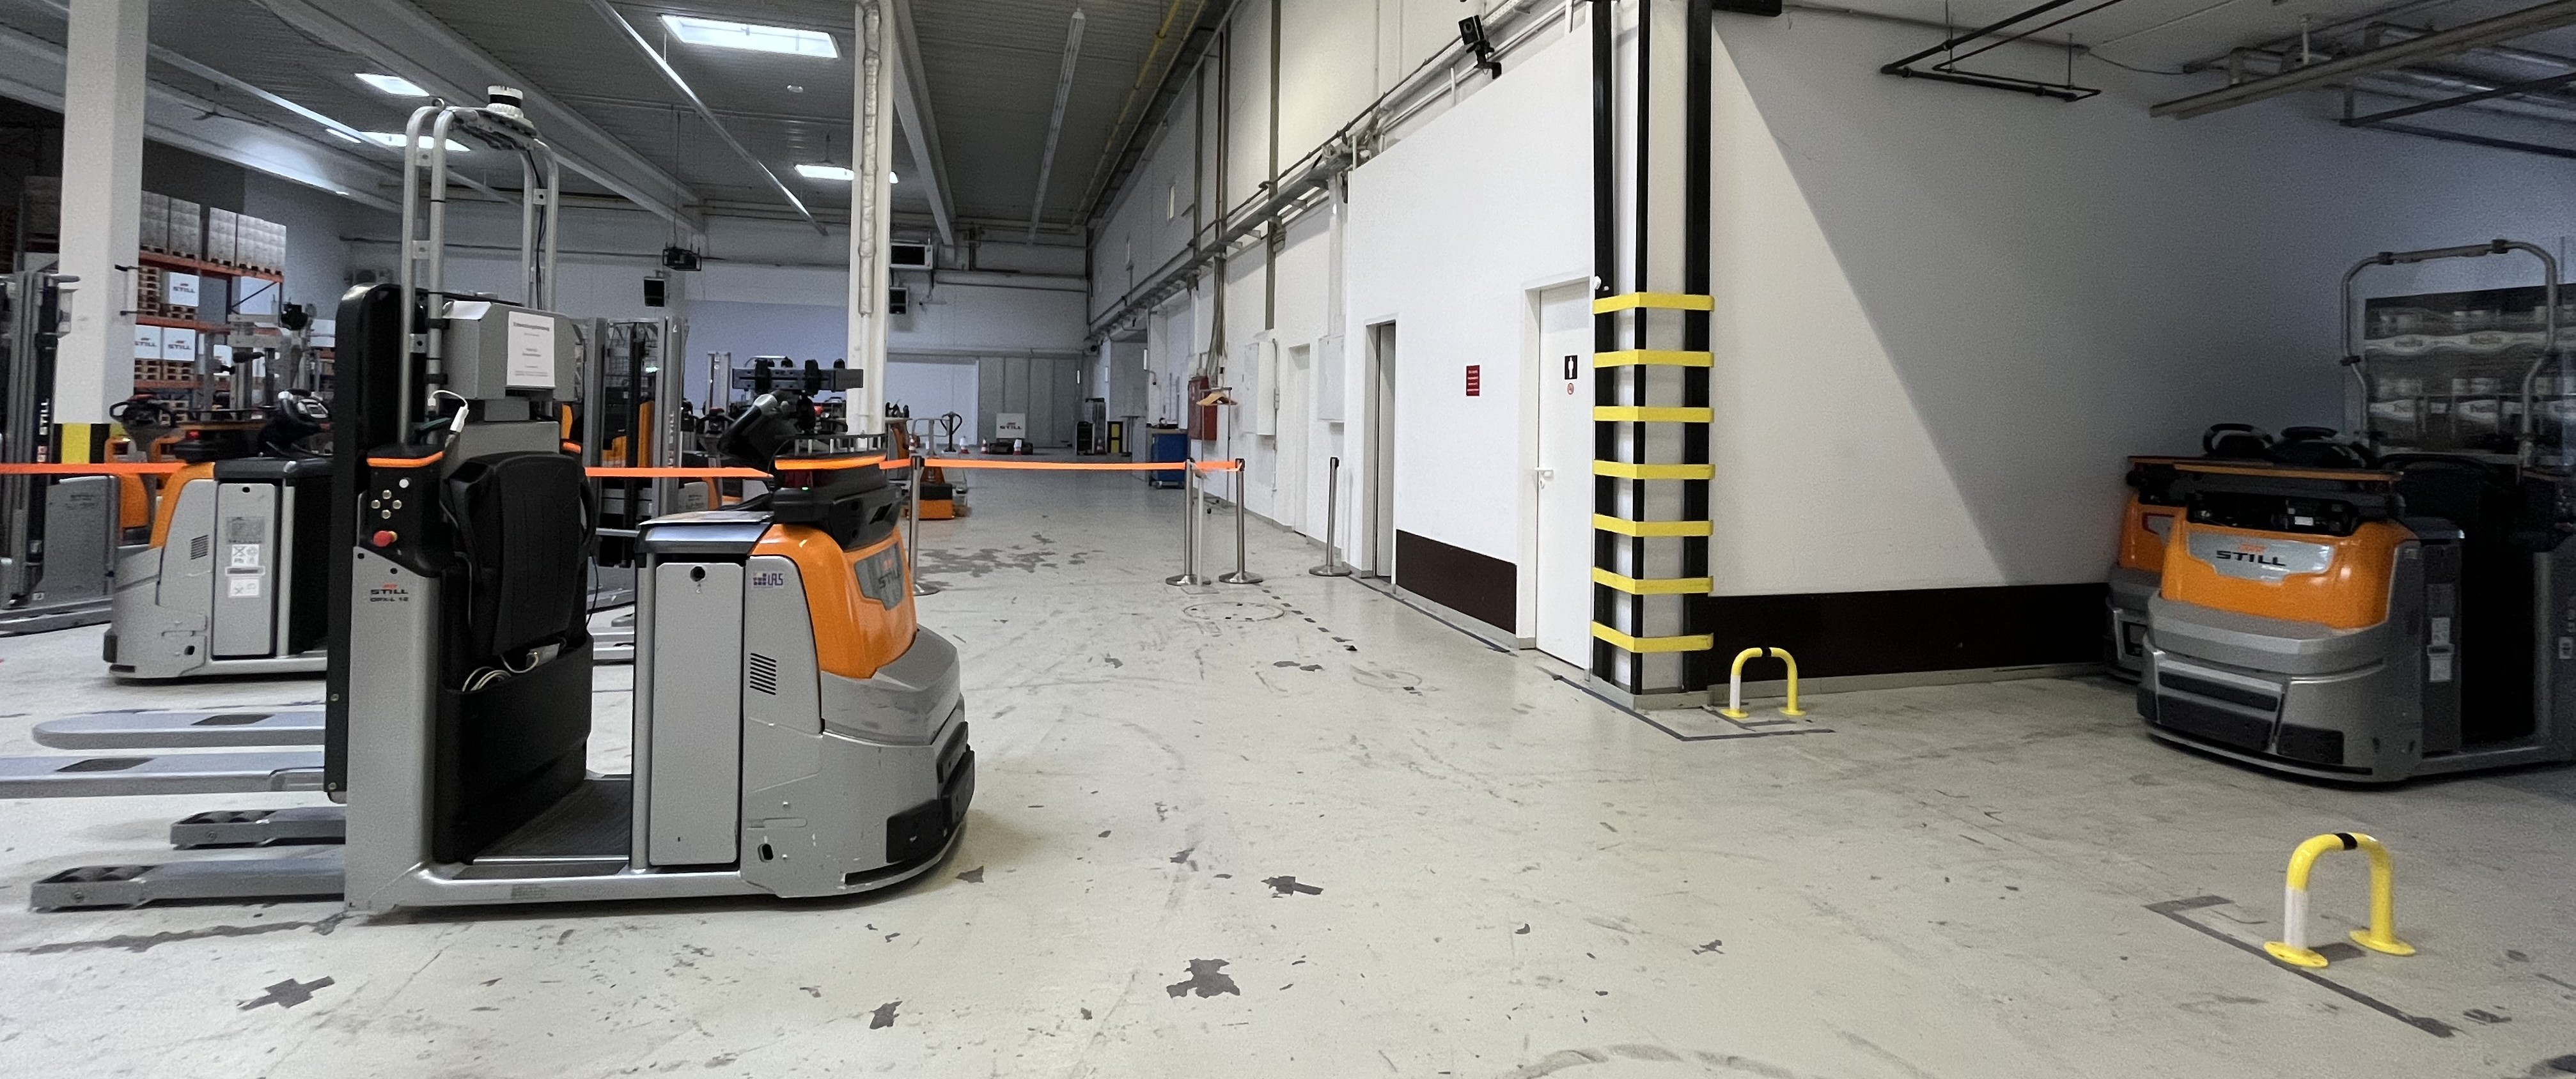
\includegraphics[width=5in]{images/Chap3/Start_Sc1.jpg} % Replace with your figure
        \caption{Environment and Start position of the Simple Test Scenario in a real warehouse
        with iGo Neo}
        \label{OptResult11}
        \end{center}    
\end{figure}

On this picture is a real warehouse where the field test took place.
The test truck is an iGo Neo and the station used is station \(Empty pallets\) at a 
global position inside the warehouse \(x = 34121\), \(y = 23752\), and \(\rho = 0.0^\circ\).
The station limits are fictional they are not outlined in the warehouse, 
but they can be seen on figure \ref{OptResult10}.
The shelf is marked by the yellow floor anchors fixed on the floor.
The environment for this test is not completely simple and empty as 
other trucks, objects, and people are in the warehouse, yet, the station is 
empty. 

\begin{figure}[H]
    \begin{center}
        \includegraphics[width=3in]{images/Chap3/Test1_transition.png} % Replace with your figure
        \caption{Truck in the simulation navigating the planned path: Transition phase}
        \label{OptResult50}
        \end{center}    
\end{figure}


\begin{figure}[H]
    \begin{center}
        \includegraphics[width=5in]{images/Chap3/Test1_real_transition.png} % Replace with your figure
        \caption{Real Truck navigating the planned path: Transition phase}
        \label{OptResult51}
        \end{center}    
\end{figure}

The Truck follows the planned path and successfully 
transitions in the transition area while changing direction to orient the 
fork to the target.

\begin{figure}[H]
    \begin{center}
        \includegraphics[width=3in]{images/Chap3/Test1_dock.png} % Replace with your figure
        \caption{Truck in the simulation navigating the planned path: Docking phase}
        \label{OptResult60}
        \end{center}    
\end{figure}


\begin{figure}[H]
    \begin{center}
        \includegraphics[width=4in]{images/Chap3/Test1_real_dock.png} % Replace with your figure
        \caption{Real Truck navigating the planned path: Docking phase}
        \label{OptResult61}
        \end{center}    
\end{figure}

The Truck arrives at the planned target and successfully 
docks the shelf with forks oriented towards it in preparation for
pickup / drop.

To summarize, for the test on the AMR, the PSO Algorithm is used. The duration of Planning of the optimized 
path was \(286ms\). 



\subsection{Complex Test Environments}
The Field-Tests in Complex Environments are conducted by placing obstacles on two sides of the 
station. 
Two test cases were carried out using two obstacle setups: Placing obstacles to the AMR's left then right
as illustrate figures \Ref{OptResult12} and \Ref{OptResult18}. 
The goal is to block one of the Transition zones, in order to test the system's flexibility,
exploration and exploitation of the transition possibilities.



\subsubsection{Obstacle Setup 1: Obstacle on the left of the AMR}

The truck was placed at position \(x = 33785\), \(y = 28845\), and \(\rho = 90.0^\circ\) as illustrated by figure 
\Ref{OptResult13}. The target is set at position \(x = 33356\), \(y = 22699\), and \(\rho = 270.0^\circ\).
The obstacle is as represented by figure \Ref{OptResult12}, a two-box block set one above the other. 
This obstacle was scanned and represented on the RACK Simulation 
Environment by its corner marked by the green arrow as illustrated by figure \Ref{OptResult13}.
The black dots seen on the same figure are scan points that represent obstacles in the warehouse. 
Usually there is more scan points, that cover for example the visible surface of an object.
For instance, the obstacle represented in figure \Ref{OptResult9} has scan points on its front side.
In the case illustrated by figure \Ref{OptResult13}, the scan points are reduced by using a RACK module 
that minimizes scan points concentrated in one area. The goal is to keep the necessary data about the surrounding 
objects and limit the amount of information to be processed 
for collision checking and path generation, thus optimizing processing time.
The optimum path is planned and the optimizer generates a pattern-based trajectory that transitions
inside the empty Transition Subpolygon. 
The generated path is illustrated in red on figure \Ref{OptResult15}. It is followed 
by the truck from the start, passing by the transition area and changing directions, and docking the 
target at the assigned position as represented on figure \Ref{OptResult16}. 

For this test setup, the planning duration of an optimum path is of \(303ms\). During this time
the optimizer processed a path that optimizes to a certain extent the path length and 
the curvature change proportionally to the path length.


\begin{figure}[H]
    \begin{center}
        \includegraphics[width=5in]{images/Chap3/Test2_ObsLeftVehic/Start_real.png} % Replace with your figure
        \caption{Environment and Start position of the Complex Test Scenario: First Obstacle setup in the warehouse}
        \label{OptResult12}
        \end{center}    
\end{figure}

\begin{figure}[H]
    \begin{center}
        \includegraphics[width=4in]{images/Chap3/Test2_ObsLeftVehic/Start_simu.png} % Replace with your figure
        \caption{Environment and Start position of the Complex Test Scenario: First Obstacle setup in the simulation}
        \label{OptResult13}
        \end{center}    
\end{figure}

\begin{figure}[H]
    \begin{center}
        \includegraphics[width=5in]{images/Chap3/Test2_ObsLeftVehic/Transition_real.png} % Replace with your figure
        \caption{Transition Position of the Complex Test Scenario: First Obstacle setup in the warehouse}
        \label{OptResult14}
        \end{center}    
\end{figure}

\begin{figure}[H]
    \begin{center}
        \includegraphics[width=4.5in]{images/Chap3/Test2_ObsLeftVehic/Transition_simu.png} % Replace with your figure
        \caption{Transition Position of the Complex Test Scenario: First Obstacle setup in the simulation}
        \label{OptResult15}
        \end{center}    
\end{figure}

\begin{figure}[H]
    \begin{center}
        \includegraphics[width=4in]{images/Chap3/Test2_ObsLeftVehic/Target_real.png} % Replace with your figure
        \caption{Target Position of the Complex Test Scenario: First Obstacle setup in the warehouse}
        \label{OptResult16}
        \end{center}    
\end{figure}

\begin{figure}[H]
    \begin{center}
        \includegraphics[width=4in]{images/Chap3/Test2_ObsLeftVehic/Target_simu.png} % Replace with your figure
        \caption{Target Position of the Complex Test Scenario: First Obstacle setup in the simulation}
        \label{OptResult17}
        \end{center}    
\end{figure}

\subsubsection{Obstacle Setup 2: Obstacle on the right of the AMR}

The truck was placed at position \(x =33891 \), \(y = 27760\), and \(\rho = 90.0^\circ\) as illustrated by figure 
\Ref{OptResult19}. The target is set at position \(x = 33492\), \(y = 22692\), and \(\rho = 270.0^\circ\).
The obstacle is a box represented by figure \Ref{OptResult18}. 
This obstacle was scanned and represented on the RACK Simulation 
Environment by its corner marked by the green arrow as illustrated by figure \Ref{OptResult19}.
The optimum path is planned and the optimizer generates a pattern-based trajectory that transitions
inside the empty Transition Subpolygon. 
The generated path is illustrated in red on figure \Ref{OptResult21}. It is followed 
by the truck from the start, passing by the transition area and changing directions, and docking the 
target at the assigned position as represented on figures \Ref{OptResult22} and \Ref{OptResult23}. 

For this test setup, the planning duration of an optimum path is of \(295ms\). During this time
the optimizer processed a path that optimizes to a certain extent the path length and 
the curvature change proportionally to the path length.

\begin{figure}[H]
    \begin{center}
        \includegraphics[width=4in]{images/Chap3/Test3/Start_real.png} % Replace with your figure
        \caption{Start Position of the Complex Test Scenario: Second Obstacle setup in the warehouse}
        \label{OptResult18}
        \end{center}    
\end{figure}

\begin{figure}[H]
    \begin{center}
        \includegraphics[width=4in]{images/Chap3/Test3/Start_simu.png} % Replace with your figure
        \caption{Start Position of the Complex Test Scenario: Second Obstacle setup in the simulation}
        \label{OptResult19}
        \end{center}    
\end{figure}

\begin{figure}[H]
    \begin{center}
        \includegraphics[width=4in]{images/Chap3/Test3/Transition_real.png} % Replace with your figure
        \caption{Transition Position of the Complex Test Scenario: Second Obstacle setup in the warehouse}
        \label{OptResult20}
        \end{center}    
\end{figure}

\begin{figure}[H]
    \begin{center}
        \includegraphics[width=4in]{images/Chap3/Test3/Transition_simu.png} % Replace with your figure
        \caption{Transition Position of the Complex Test Scenario: Second Obstacle setup in the simulation}
        \label{OptResult21}
        \end{center}    
\end{figure}

\begin{figure}[H]
    \begin{center}
        \includegraphics[width=4in]{images/Chap3/Test3/Target_Real.png} % Replace with your figure
        \caption{Target Position of the Complex Test Scenario: Second Obstacle setup in the warehouse}
        \label{OptResult22}
        \end{center}    
\end{figure}

\begin{figure}[H]
    \begin{center}
        \includegraphics[width=4in]{images/Chap3/Test3/Target_simu.png} % Replace with your figure
        \caption{Target Position of the Complex Test Scenario: Second Obstacle setup in the simulation}
        \label{OptResult23}
        \end{center}    
\end{figure}



\subsection{Discussion of the results}

The Pattern-based path planning approach was tested in 3 different scenarios.
The PSO Algorithm was used for the 3 scenarios and successfully generated feasible paths for each 
test case. In the cases where obstacles were presented to the station the optimizer 
showcased the obstacle avoidance feature by rejecting colliding paths and opting for optimum
candidates that scored the least fitness values among the 200 generated individuals.
The previous test cases and events proved that the proposed approach is a simple and feasible 
solution to the docking process.
While the planning time in the RACK Simulation Environment was as low as \(59ms\) for the Simple Environment
and \(67ms\) for the Complex Environment, the field-testing scenarios scored planning times of 
\(286ms\) up to \(303ms\). 
This duration is significantly higher than the duration 
on the simulation. This is due to the high number of objects surrounding the vehicle which are 
represented by scan points that the truck needs to check for collisions for every path candidate.  
The traveled path can be shorter: the used Evaluation approach favors the optimization of the 
curvature term over the length, in other words, a longer path is better than a curved path.
This minimizes the curvature but creates long paths that have room for improvement. 

\section{Summary of Contributions and Reflections}
The goals set out for this thesis have been successfully achieved. A solution was developed that generates 
repeatable paths adhering to a predefined pattern, ensuring compliance with the specific layout and dimensions 
of the destination station. The solution is station-related, meaning it is tailored to the available space and 
dimensions of each station, allowing for precise accuracy in docking. Paths are generated within the goal's 
frame of reference, ensuring precision upon arrival. Additionally, optimization was achieved by focusing on 
both path length and curvature, utilizing metaheuristic algorithms to avoid obstacles while aligning with the 
kinematic constraints of the vehicle. This ensures an optimal and efficient route while respecting the physical 
limitations of the truck.

Several key gaps found in the literature, particularly related to intensive computational demands and long 
processing times in existing mobile robot path planning methods, have been addressed. The developed approach 
significantly reduces planning time, achieving times between 40 and 50 milliseconds in simulation and around 
300 milliseconds in field tests. In contrast, planning times in the literature range from 13 to 31 seconds 
(as outlined in Chapter 2, Section 4). Real-world challenges were addressed by simulating real obstacles and 
incorporating them into field tests. The pattern-based path generation approach also complies with the vehicle's 
kinematic constraints, such as turning radius, by limiting curvature, which ensures both computational efficiency 
and practical applicability in real-world scenarios.

The solution also fulfills the initial motivations by providing explainable and predictable paths. Maneuvering 
and direction changes are clearly interpretable by human operators, ensuring transparency in the system’s behavior. 
The decision-making process is also explainable, with the optimizer’s parameters—path length and curvature—clearly 
defined and weighted. The ease of commissioning is preserved, as the system is designed to recognize stations 
easily and is adaptable to any station, regardless of its orientation (as demonstrated in the tests conducted on 
two stations in Chapter 4). By addressing these key points, the solution enhances customer trust and confidence 
while maintaining both autonomy and operational efficiency.

\subsection*{Conclusion}
In this chapter, the proposed solution was rigorously tested and validated through a series of evaluations, 
beginning with path creation and extending to path optimization and real-world field-testing. 
The results demonstrated the effectiveness of the solution in creating, evaluating, and optimizing paths, 
with each stage providing valuable insights into its performance. The field tests conducted in a simple 
environment using an Autonomous Mobile Robot (AMR) confirmed that the proposed solution could be effectively 
deployed in practical scenarios. The discussion highlighted key takeaways, underscoring the robustness 
and applicability of the solution in real-world settings.
% \input{chapters/chap4.tex}

\fancyhead[R]{}

% General Conclusion
\chapter*{General conclusion}
\addcontentsline{toc}{chapter}{General conclusion}

This project has explored the complex and rapidly evolving field of intralogistics, focusing on the optimization of 
local path planning for the autonomous forklifts' AMRs produced by STILL. The technique introduced by this thesis 
concerns a specific part of the global path that allows the AMR to properly dock the target. The work was structured 
across four key chapters, each building towards a comprehensive understanding and solution to the challenges faced 
in modern industrial environments.

Chapter 1 provided a thorough introduction to the host company, STILL, detailing its structure, and contributions 
to the intralogistics industry. By outlining the project’s context, motivations, and core problematics, this chapter 
laid the groundwork for understanding the broader objectives and the specific goals of this thesis, particularly 
in optimizing path planning near pallet stations.

\noindent Chapter 2 delved into the state-of-the-art literature, offering a review of existing solutions in autonomous 
robotics and path planning. This chapter underscored the gaps in current approaches and the opportunity for 
innovative optimization strategies, especially in environments like brownfield warehouses, where challenges such 
as disorganization and uneven terrain present significant obstacles to automation.

\noindent Chapter 3 marked the technical core of the thesis, focusing on the mathematical and geometric principles behind 
the proposed solution. The exploration of splines in path planning, combined with the geometric division of 
warehouse stations into transition zones, highlighted the need for precision and flexibility in near-field 
navigation. Through a detailed discussion of path discrimination and optimization methods, this chapter 
demonstrated how smart algorithms can enable autonomous vehicles to plan and execute efficient routes 
while avoiding obstacles.

\noindent Finally, Chapter 4 presented the practical implementation of these ideas in the RACK framework and simulation 
system, detailing the tests conducted on autonomous forklifts and the results obtained. The successful trials 
showcased the efficacy of the optimized local path planning approach, proving that the developed solution is 
not only theoretically sound but also practically applicable in real-world scenarios.

In conclusion, this thesis has demonstrated that the desired optimizations can be be achieved by implementing less sophisticated path planning techniques and without the need to implement over-kill solutions like AI-based. The proposed approach contributes to the growing body of knowledge in autonomous robotics and intralogistics, offering a solution that enhances safety, efficiency, and predictability which opens the door for customers and potential customers to trust the presence of the autonomous forklifts in complex intralogistics environments with the european standards.

% Bibliography & Netography

\renewcommand\bibname{Bibliography}

\begin{thebibliography}{9}
\addcontentsline{toc}{chapter}{Bibliography} % to add it to the tables of contents
% TODO: date de consultation websites
%---------------------chap1
\bibitem[1] {R1}
KION group website. URL: \url{https://www.kiongroup.com/en/About-us/Management/} consulted on 19/07/2024

\bibitem[2] {R2}
KION group website. URL: \url{https://www.kiongroup.com/en/About-us/KION-at-a-glance/} consulted on 19/08/2024

\bibitem[3] {R3}
STILL website, iGo Neo page. URL: \url{https://www.still.de/en-DE/trucks/new-trucks/order-pickers/opx-20-25-igo-neo.html}

\bibitem[4] {R4}
STILL website, iGo Neo page. URL: \url{https://www.still.de/en-DE/trucks/new-trucks.html}

\bibitem[5] {R5}
iGo Neo datasheet. URL: \url{data.still.de/assets/products/Vehicles/Order_Pickers/OPX_iGo_neo/pdfs/OPX_EN_TD.pdf?mod=1681891889&s=baf72412ac0d268f13b017603ca95ea2}

\bibitem[6] {R6}
Agile Scrum article. URL: \url{https://top20review.com/phuong-phap-agile/}

\bibitem[7] {R7}
Giuseppe Fragapane, René de Koster, Fabio Sgarbossa, Jan Ola Strandhagen,
Planning and control of autonomous mobile robots for intralogistics: Literature review 
and research agenda, European Journal of Operational Research, Volume 294, Issue 2, 2021,
Pages 405-426, ISSN 0377-2217, https://doi.org/10.1016/j.ejor.2021.01.019.

\bibitem[8] {R8}
Moshayedi, Ata Jahangir \& Liao, Liefa \& Kolahdooz, Amin. (2021). 
Gentle Survey on MIR Industrial Service Robots: Review \& Design. 10. 

\bibitem[9] {R9}
AMR vs. AGV Figure, Vecna Robotics Website. URL: \url{https://www.vecnarobotics.com/amr-vs-agv/}, 
consulted on 28.07.2024

\bibitem[10] {R10}
Lixing Liu, Xu Wang, Xin Yang, Hongjie Liu, Jianping Li, Pengfei Wang,
Path planning techniques for mobile robots: Review and prospect,
Expert Systems with Applications, Volume 227, 2023, 120254, ISSN 0957-4174,
https://doi.org/10.1016/j.eswa.2023.120254.

\bibitem[11] {R11}
Marín, Pablo \& Hussein, Ahmed \& Martín Gómez, David \& de la Escalera, Arturo. (2018). 
Global and Local Path Planning Study in a ROS-Based Research Platform for Autonomous Vehicles. 
Journal of Advanced Transportation. 2018. 1-10. 10.1155/2018/6392697. 

\bibitem[12] {R12}
Mohd. Nayab Zafar, J.C. Mohanta,
Methodology for Path Planning and Optimization of Mobile Robots: A Review,
Procedia Computer Science,
Volume 133,
2018,
Pages 141-152,
ISSN 1877-0509,
https://doi.org/10.1016/j.procs.2018.07.018.

\bibitem[13]{R13}
Zhang B, Zhu D. A new method on motion planning for mobile robots using jump point search 
and Bezier curves. International Journal of Advanced Robotic Systems. 2021;18(4). doi:10.1177/17298814211019220

\bibitem[14]{R14}
H. -T. Lee, H. -M. Choi, J. -S. Lee, H. Yang and I. -S. Cho, "Generation of Ship’s Passage Plan Using 
Data-Driven Shortest Path Algorithms," in IEEE Access, vol. 10, pp. 126217-126231, 2022, 
doi: 10.1109/ACCESS.2022.3225571.

\bibitem[15]{R15}
Sertac Karaman and Emilio Frazzoli. 2011. Sampling-based algorithms for optimal motion planning. 
Int. J. Rob. Res. 30, 7 (June      2011), 846–894. https://doi.org/10.1177/0278364911406761

\bibitem[16]{R16}
c. Ichnowski and c. Alterovitz, "Parallel sampling-based motion planning with superlinear speedup," 
2012 IEEE/RSJ International Conference on Intelligent Robots and Systems, Vilamoura-Algarve, 
Portugal, 2012, pp. 1206-1212, doi: 10.1109/IROS.2012.6386194.

\bibitem[17]{R17}
A. Elshamli, H. A. Abdullah and S. Areibi, "Genetic algorithm for dynamic path planning," 
Canadian Conference on Electrical and Computer Engineering 2004 (IEEE Cat. No.04CH37513), 
Niagara Falls, ON, Canada, 2004, pp. 677-680 Vol.2, doi: 10.1109/CCECE.2004.1345203.

\bibitem[18]{R18}
Q. Jin, C. Tang and W. Cai, "Research on Dynamic Path Planning Based on the Fusion Algorithm 
of Improved Ant Colony Optimization and Rolling Window Method," in IEEE Access, vol. 10, pp. 
28322-28332, 2022, doi: 10.1109/ACCESS.2021.3064831

\bibitem[19]{R19}
Liu, Li-sang, Lin, Jia-feng, Yao, Jin-xin, He, Dong-wei, Zheng, Ji-shi, Huang, Jing, Shi, 
Peng, Path Planning for Smart Car Based on Dijkstra Algorithm and Dynamic Window Approach, 
Wireless Communications and Mobile Computing, 2021, 8881684, 12 pages, 2021. https://doi.org/10.1155/2021/8881684

\bibitem[20]{R20}
S. H. Tang, F. Kamil, W. Khaksar, N. Zulkifli and S. A. Ahmad, "Robotic motion planning in unknown 
dynamic environments: Existing approaches and challenges," 2015 IEEE International Symposium on Robotics 
and Intelligent Sensors (IRIS), Langkawi, Malaysia, 2015, pp. 288-294, doi: 10.1109/IRIS.2015.7451627. 

\bibitem[21]{R21}
Alterovitz, R., Koenig, S., \& Likhachev, M. (2016). Robot Planning in the Real World: Research Challenges and Opportunities. 
AI Magazine, 37(2), 76-84. https://doi.org/10.1609/aimag.v37i2.2651



\end{thebibliography}




\newpage
%\pagenumbering{alph}
\chapter* {Annexes}
\addcontentsline{toc}{chapter}{Annexes}





\end{document}